\documentclass[dvipdfmx]{beamer}
\documentclass[dvipdfmx]{beamer}
\input
\usetheme{Madrid}

\title{Current Status}
\author{Kentaro Inoue}
\date{\today}

\begin{document}
\maketitle

\begin{frame}{Items}
  \begin{itemize}
  \item Scaling factors
    \begin{itemize}
    \item Trigger and DAQ page.\pageref{page:Trig} 
    \item Beam Line Analysis (Number of kaon) page.\pageref{page:BL}
    \end{itemize}
  \item Detector performance
    \begin{itemize}
    \item CDS page.\pageref{page:CDS}
    \item NC page.\pageref{page:NC}
    \end{itemize}
  \end{itemize}
\end{frame}

\begin{frame}{Scaling Factor}
  \begin{itemize}
  \item Luminosity
    \begin{eqnarray*}
      L=N_{beam}N_{target}Eff_{DAQ}Eff_{Trigger}=5870 \pm 150 \\
      N_{target}=l(10cm)\times \rho (0.169g/cm^3) \times N_{A}/N_{d}\\
      N_{beam} N_{DAQ} N_{trigger} \mbox{were estimated run-by-run.}\\
    \end{eqnarray*}
  \item Neutron Efficiency\\
    $Eff_{NC}=0.317\pm 0.016$ by $K^-d\rightarrow K^0 n$ reaction (RUN62)\\
    $Overkill_{\overline{CVC\cup PC}}=0.081\pm0.007$ (RUN78)
  \item CDC efficeincy\\
    RUN68 IH and CDH was used as trigger counters $\sim 0.977\pm 0.004$\\
    RUN78 was estimated from the value that CDC layer1 was used instead of IH.
  \end{itemize}
\end{frame}


\begin{frame}
  \label{page:Trig}
  { \Huge Trigger and DAQ eff.}
\end{frame}
\begin{figure}[htbp]
  \centering
  \includegraphics[width=14cm]{pic/experiment/trigger.eps}
  \caption{
    Schematic view of trigger scheme
  }
  \label{fig:trigger}
\end{figure}


\begin{frame}
  \label{page:BL}
  { \Huge Beam Line Analysis \newline (Number of Kaon)}
\end{frame}
\begin{frame}{Kaon Number}
  \begin{tabular}{cc}
    \begin{minipage}{0.5\hsize}
      \begin{figure}
        Relative Ratio
        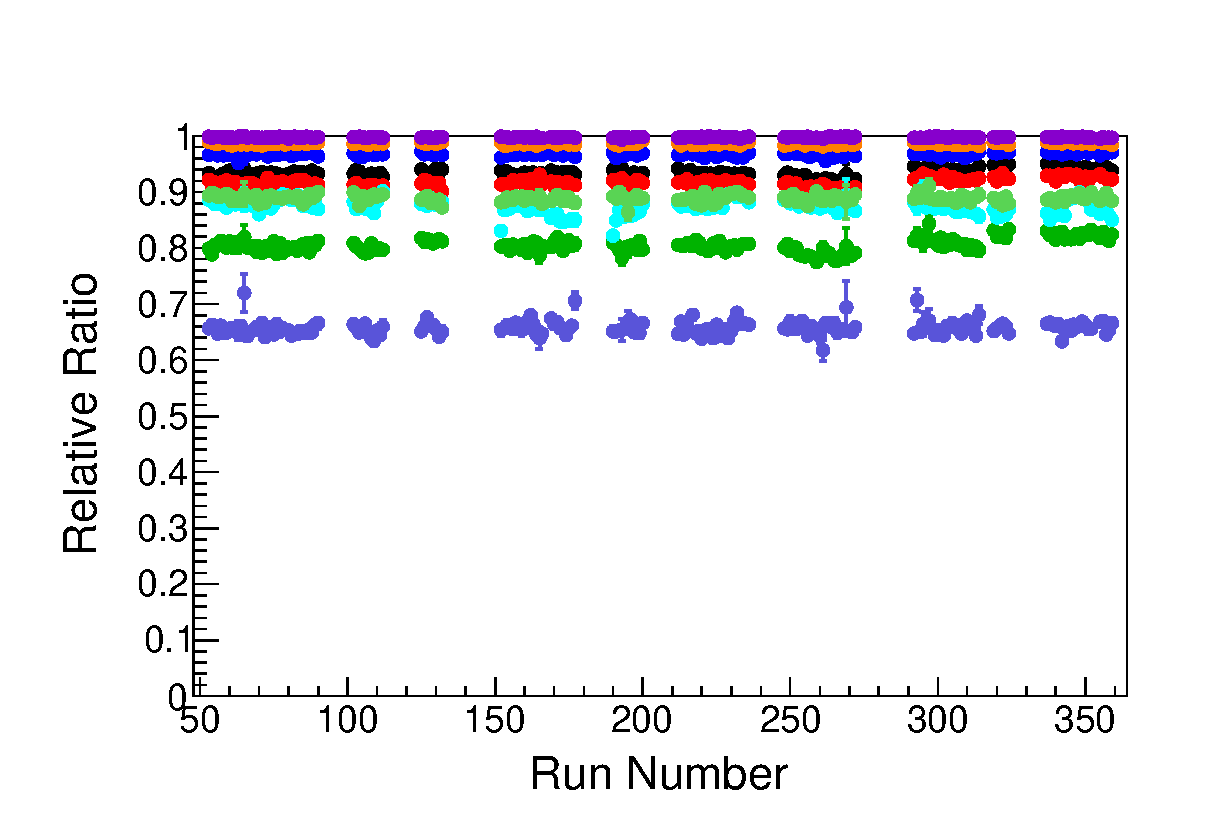
\includegraphics[width=5cm]{../pic/Run78/BL/relative_ratio.eps}
      \end{figure}
    \end{minipage}

    \begin{minipage}{0.5\hsize}
      \begin{figure}
        Survival Ratio
        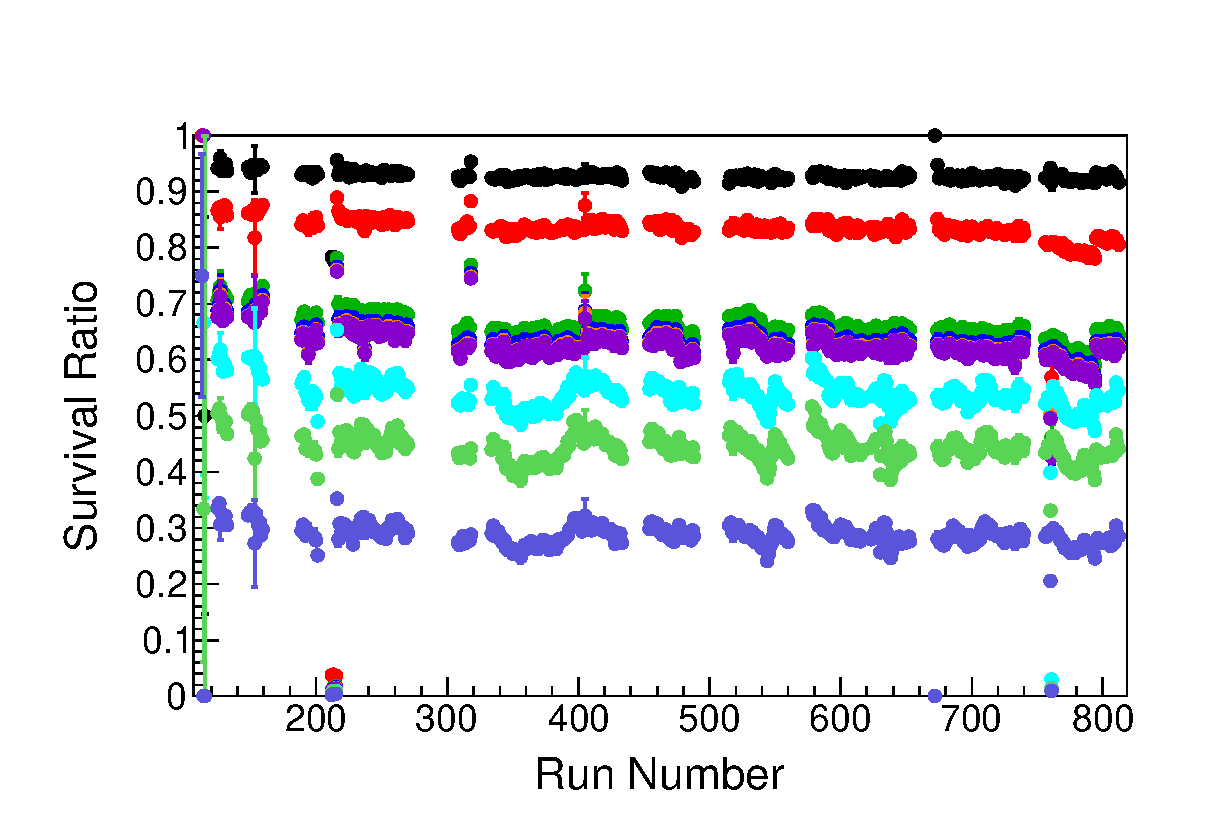
\includegraphics[width=5cm]{../pic/Run78/BL/survival_ratio.eps}
      \end{figure}
    \end{minipage}
  \end{tabular}

  \begin{tabular}{cc}
    \begin{minipage}{0.5\hsize}
      \begin{figure}
        Irradiated Kaon Number
        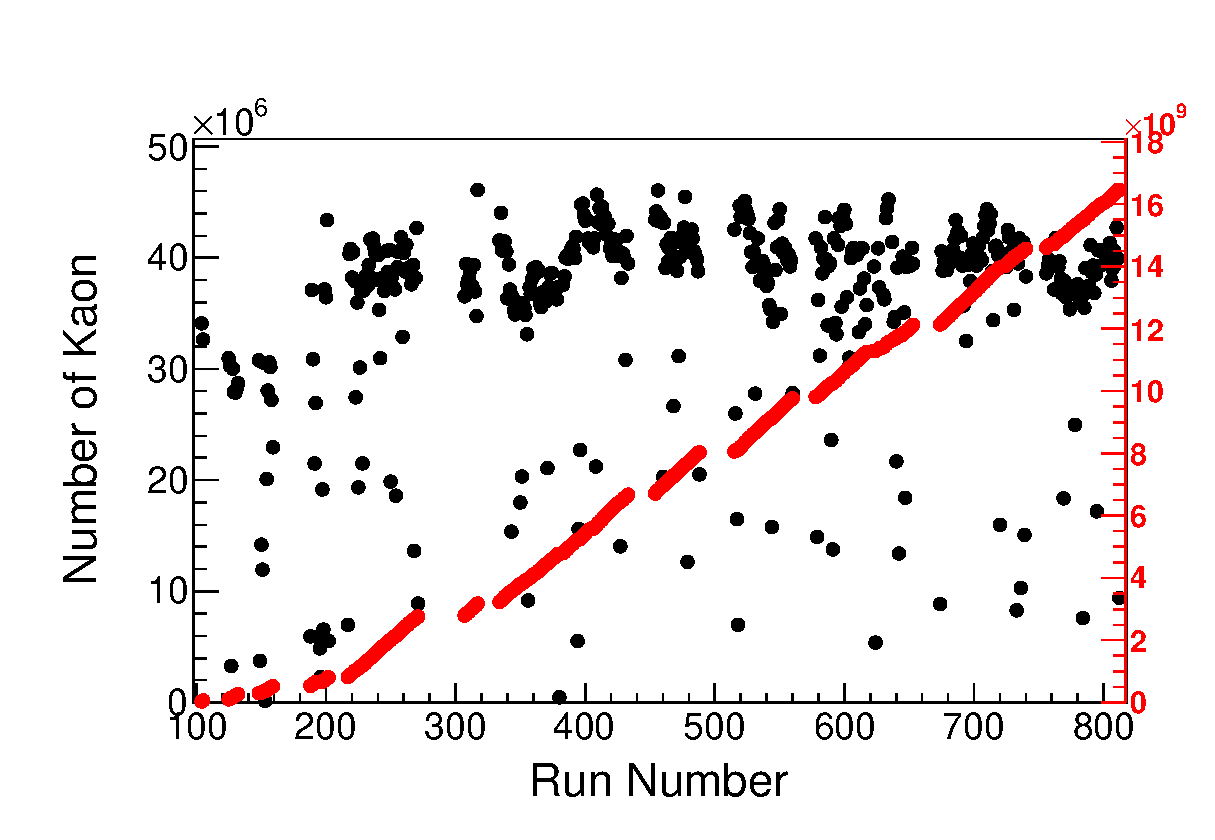
\includegraphics[width=5cm]{../pic/Run78/BL/Knum.eps}
      \end{figure}
    \end{minipage}

    \begin{minipage}{0.5\hsize}
      $15.8\pm0.3$ G kaon were irradiated on liquid-deuterium target.
    \end{minipage}
  \end{tabular}
\end{frame}

\subsection{BHD and T0}
The beam particles are kaon is confirmed by the TOF method using beamline hodoscope detector (BHD) and time-zero counter (T0) in the offline analysis.
The T0 is located immediately downstream of the AC.
The BHD is located between the D5 and D4 magnets, approximately 7.7m upstream of T0, i.e. the flight length is 7.7m.

The T0 is a 5-segment plastic scintillation counter array 160mm (high) $\times$ 32mm (width) $\times$ 10mm (thick), with an effective area of 160mm $\times$ 160mm.
The T0 is installed rotated 45 degrees with respect to the beam direction as the beam is horizontally spread at the T0.
A counter uses the Saint-Gobain BC420 scintillator and attached readout which is 3/4 inch Hamamatsu H6612B photomultipliers to both sides of the scintillator.

The BHD is a 20-segment plastic scintillation counter array 160mm (high) $\times$ 20mm (width) $\times$ 5mm (thick), with an effective area of 200mm (horizontal) $\times$ 160mm (vertical).
A counter uses the same photomultipliers as the T0 counter.
The BHD is installed at the most upstream of the beamline and the number of beams per spill is a few M ($\times 10^6$)events,
so the photomultipliers are attached high voltage booster to the last three dynodes to avoid gain drop due to high current by high rate beam.

\subsection{Beam line chamger}
\begin{figure}[htbp]
  \centering
  \begin{tabular}{ccc}
    \begin{minipage}{0.33\hsize}
      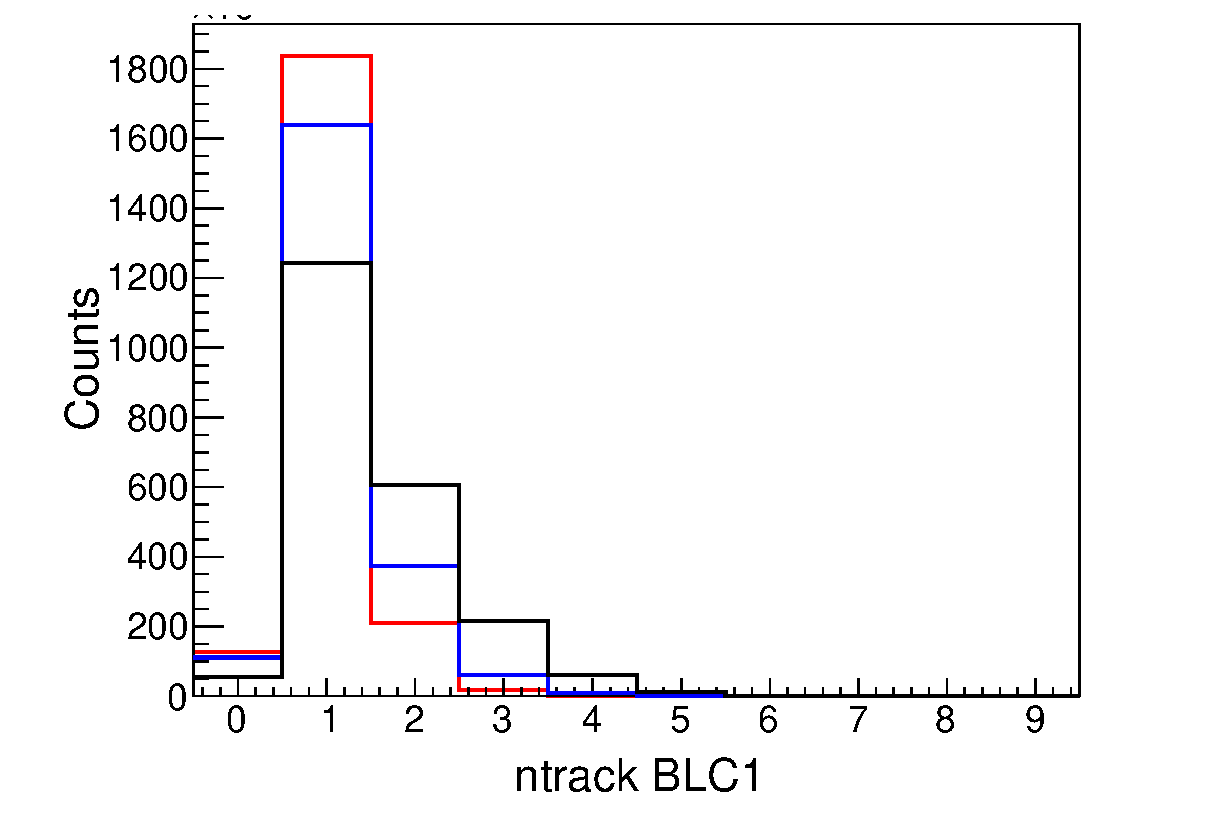
\includegraphics[width=4cm]{../pic/Run78/BL/nBLC1.eps}
    \end{minipage}
    \begin{minipage}{0.33\hsize}
      \includegraphics[width=4cm]{../pic/Run78/BL/BLC1_time.eps}
    \end{minipage}
    \begin{minipage}{0.33\hsize}
      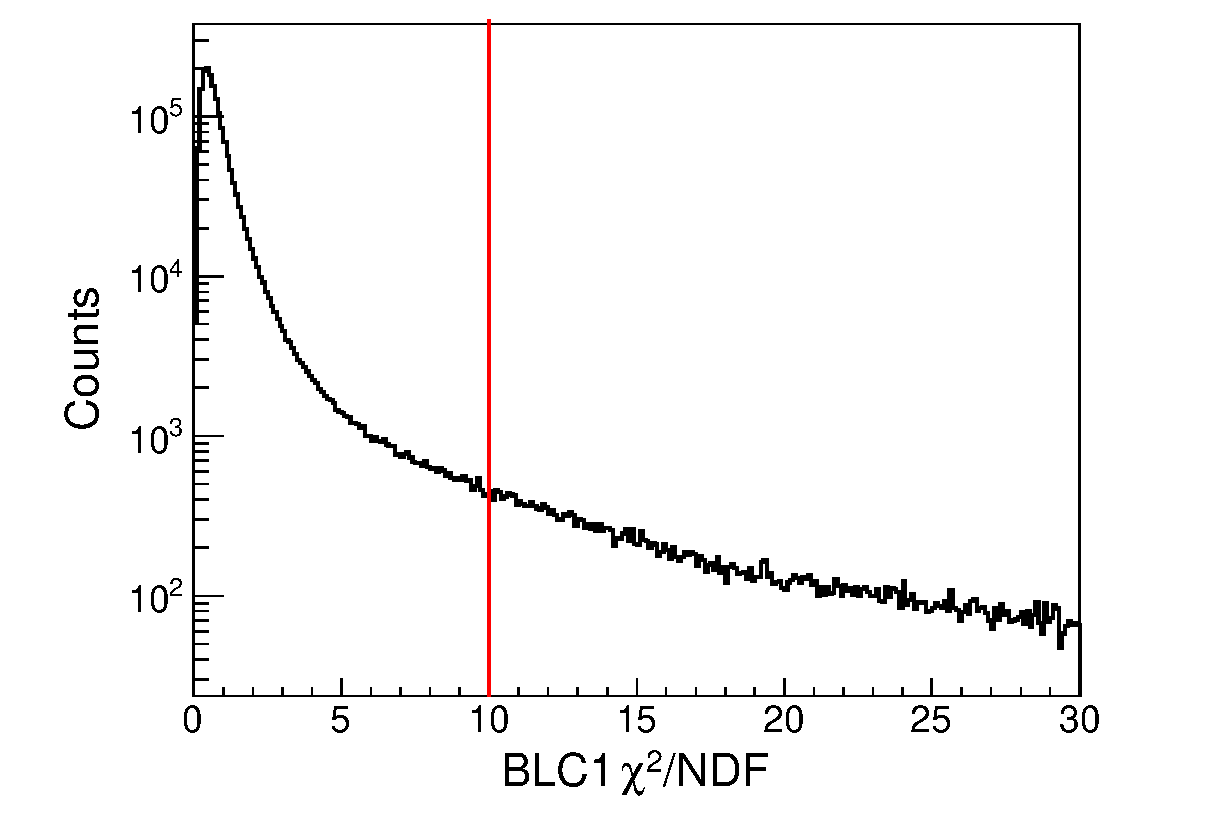
\includegraphics[width=4cm]{../pic/Run78/BL/BLC1_chi2.eps}
    \end{minipage}
  \end{tabular}
  
  \begin{tabular}{ccc}
    \begin{minipage}{0.33\hsize}
      \includegraphics[width=4cm]{../pic/Run78/BL/nBLC2.eps}
    \end{minipage}
    \begin{minipage}{0.33\hsize}
      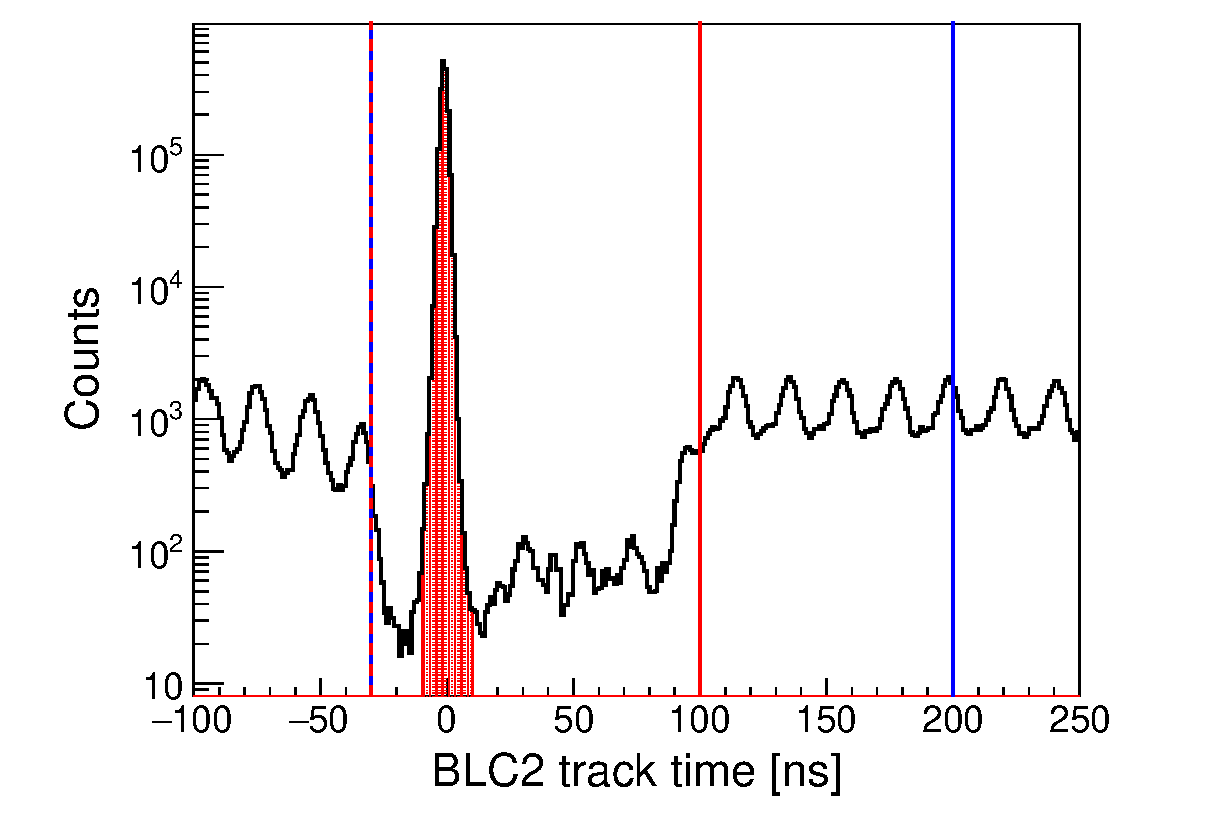
\includegraphics[width=4cm]{../pic/Run78/BL/BLC2_time.eps}
    \end{minipage}
    \begin{minipage}{0.33\hsize}
      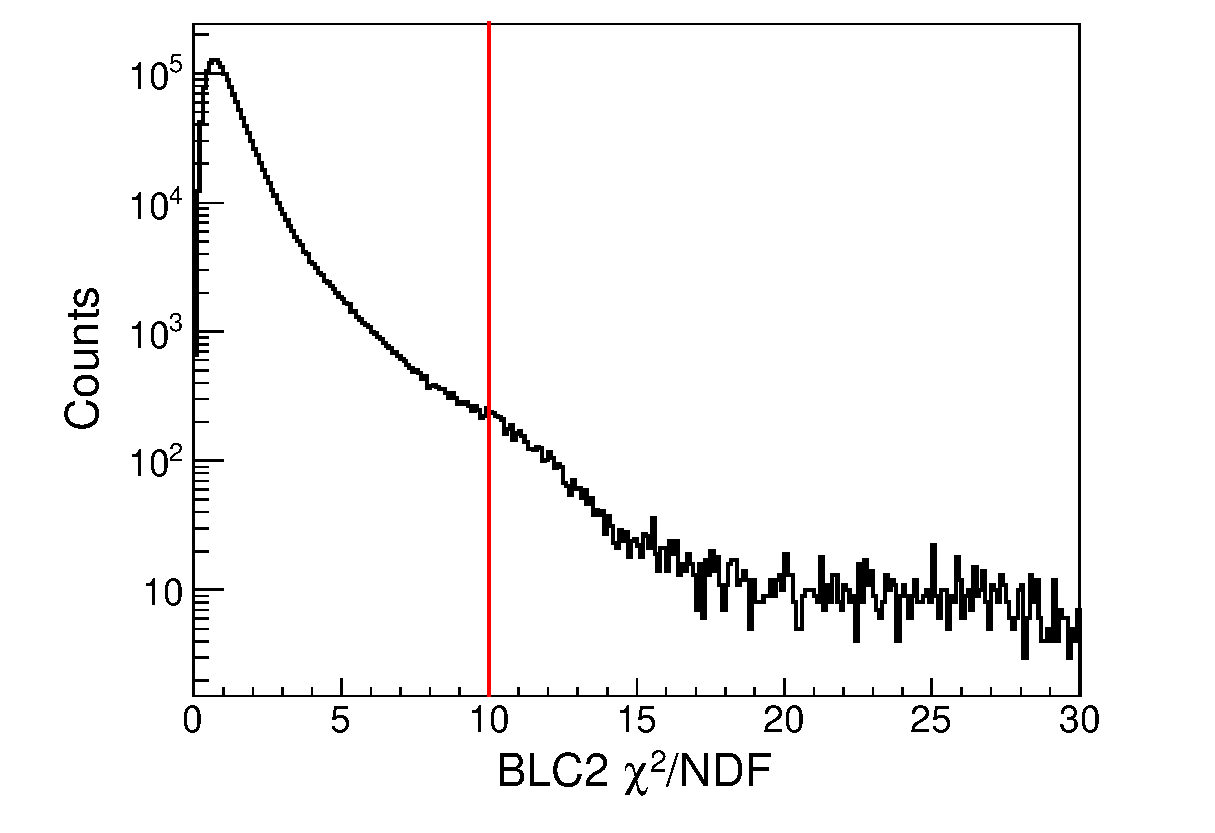
\includegraphics[width=4cm]{../pic/Run78/BL/BLC2_chi2.eps}
    \end{minipage}
  \end{tabular}
  
  \begin{tabular}{ccc}
    \begin{minipage}{0.33\hsize}
      \includegraphics[width=4cm]{../pic/Run78/BL/nBPC.eps}
    \end{minipage}
    \begin{minipage}{0.33\hsize}
      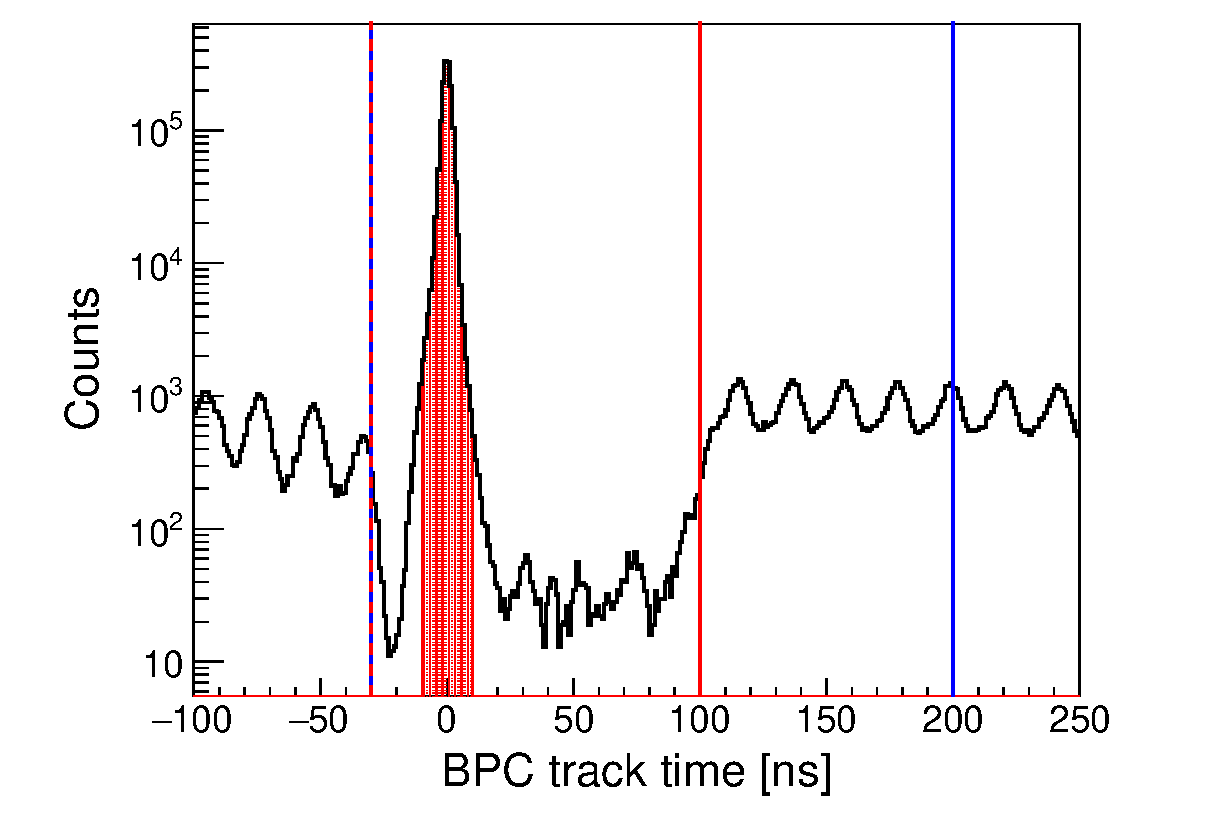
\includegraphics[width=4cm]{../pic/Run78/BL/BPC_time.eps}
    \end{minipage}
    \begin{minipage}{0.33\hsize}
      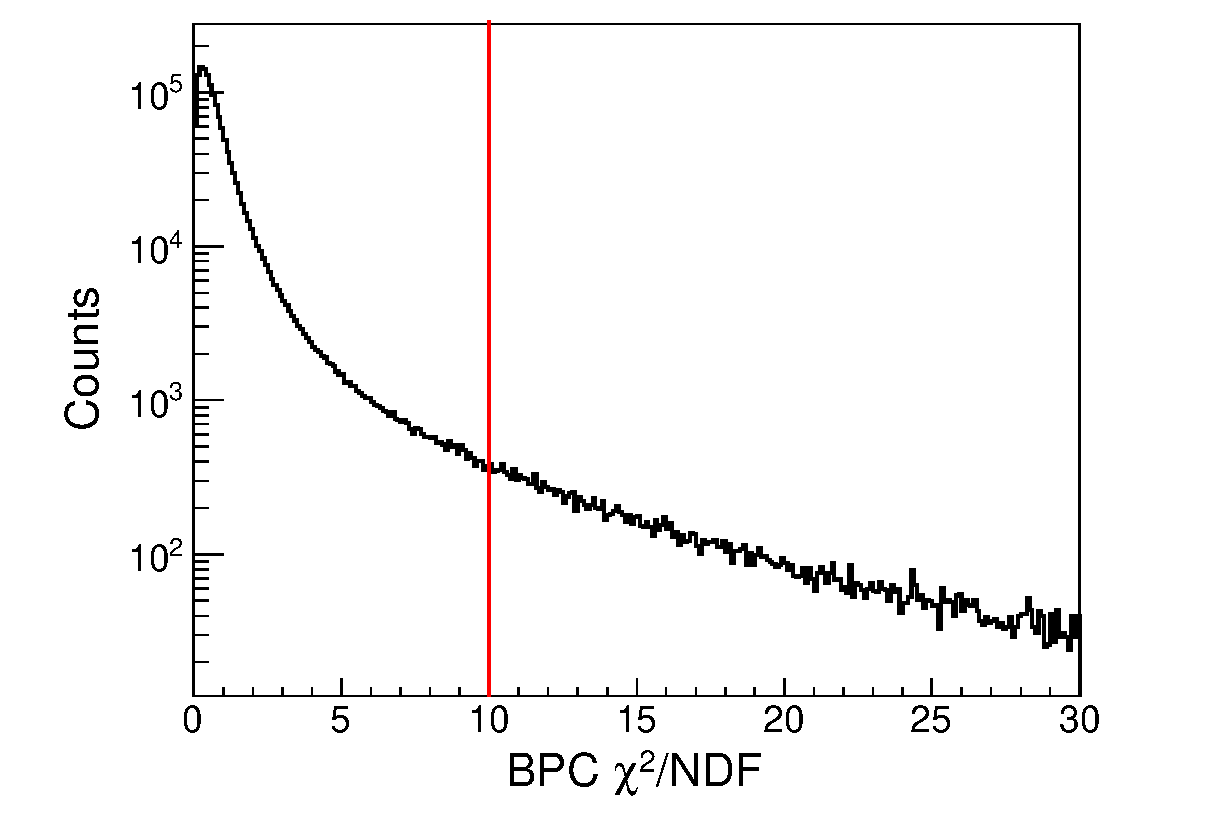
\includegraphics[width=4cm]{../pic/Run78/BL/BPC_chi2.eps}
    \end{minipage}
  \end{tabular}
  \caption{
    The left, the middle and the right figures show the number of tracks, track time and $\chi/NDF$, respectively.
    Color plots in the left figure indicate some time window.
    % Black, blue, red indicate all, $-30\sim200$[ns], $-30\sim100$[ns], respectively.
    The above, the middle and the down figures represent BLC1, BLC2 and BPC, respectively.
    The BPC was described after.
  }
  \label{fig:BLC_etc}
\end{figure}
BLC1 and BLC2 were installed upstream and downstream of the D5 magnet, respectively to measure beam momentum using the transfer matrix of the D5 magnet.
These are planer the type drift chamber whose drift length was calculated using the X-T map, which was the integration of drift time.
The track time of BLC was estimated from timing signals of pair plane due to constant drift length.
SX beam has RF-structure seems like the center figures of Fig\ref{fig:BLC_etc}, so we select synchronization about beam which indicates the red hatched region.
The left figures represent the number of tracks, in which black, blue, and red indicate time window of all, $-30\sim100$[ns], and $-30\sim200$[ns], respectively.
We select 1track events in red time window selection to keep statistics.
The right figures show $\chi^2/NDF$ distribution after 1track selection.
We accepted $\chi^2/NDF<10$ events as good track.

\begin{frame}{Beam momentum analysis by D5}
  \begin{tabular}{cc}
    \begin{minipage}{0.5\hsize}
      \begin{figure}
        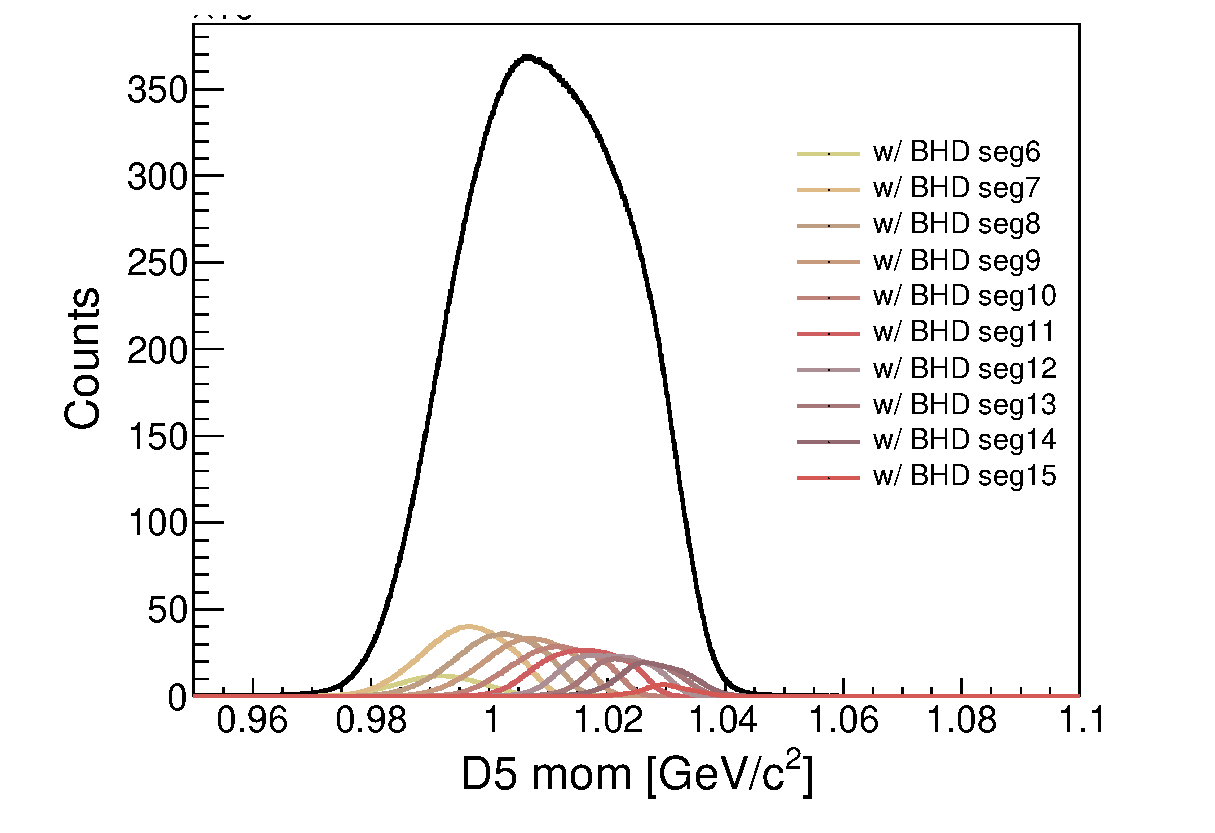
\includegraphics[width=5cm]{../pic/Run78/BL/D5_mom.eps}
      \end{figure}
    \end{minipage}

    \begin{minipage}{0.5\hsize}
      \begin{figure}
        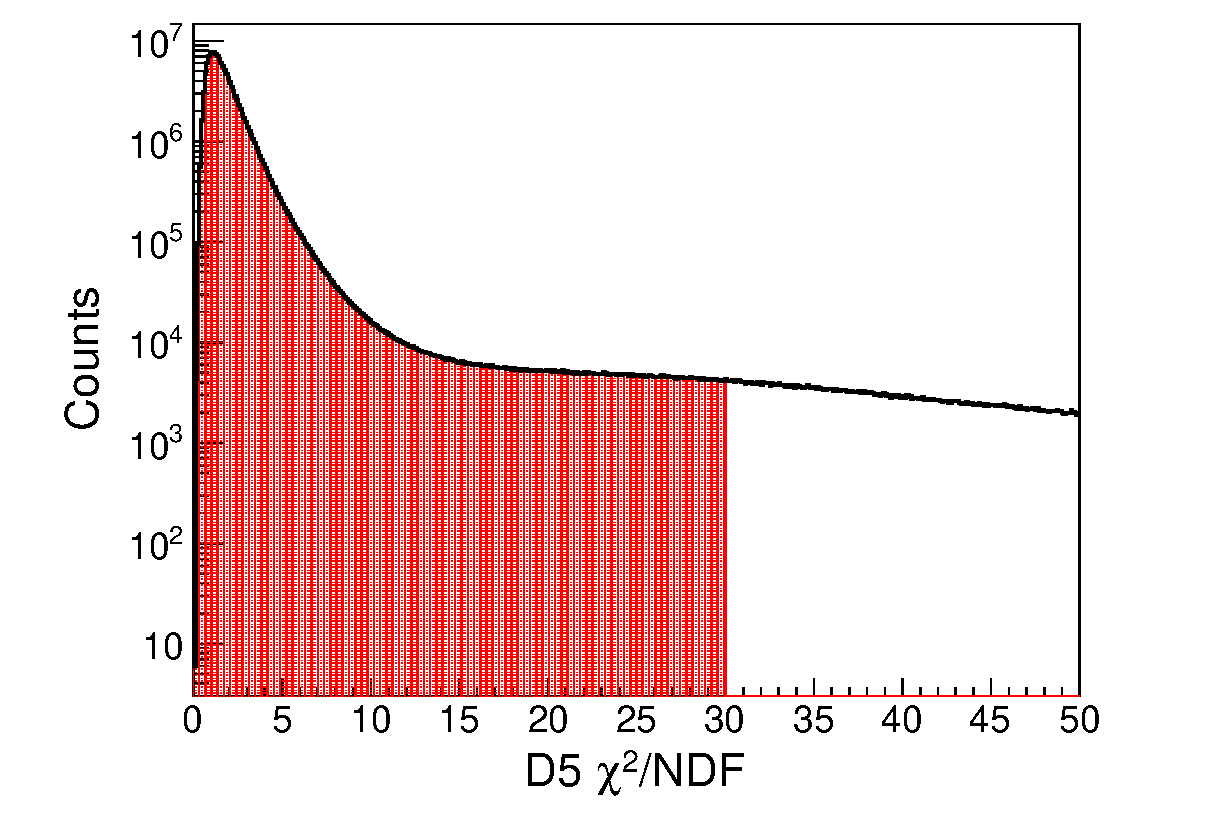
\includegraphics[width=5cm]{../pic/Run78/BL/D5_chi2.eps}
      \end{figure}
    \end{minipage}
  \end{tabular}


  \begin{tabular}{cc}
    \begin{minipage}{0.5\hsize}
      \begin{figure}
        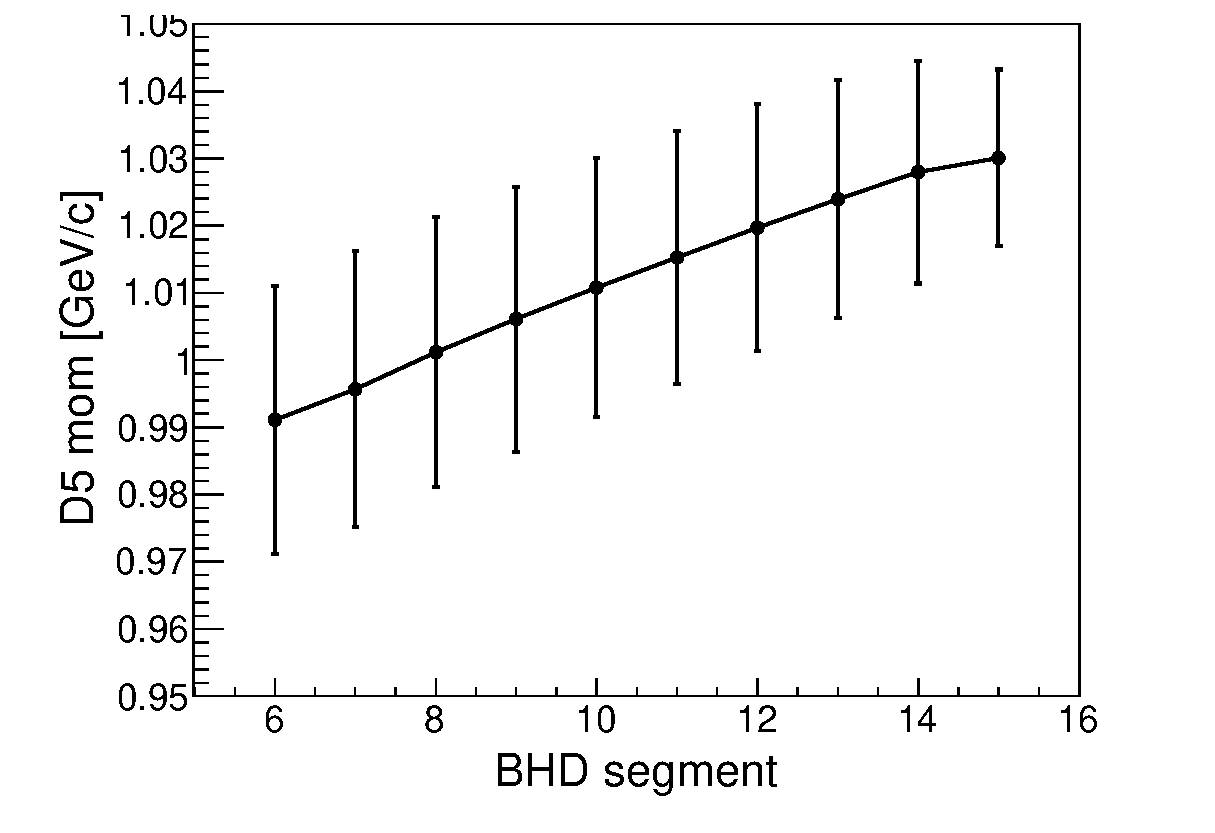
\includegraphics[width=5cm]{../pic/Run78/BL/D5_mom_BHDseg.eps}
      \end{figure}
    \end{minipage}

    \begin{minipage}{0.5\hsize}
      D5 momentum has a correlation about BHD segment.
    \end{minipage}
  \end{tabular}



\end{frame}

\subsection{BLC2-BPC matching}
\begin{figure}[htpb]
  \centering
  \begin{tabular}{cc}
    \begin{minipage}{0.5\hsize}
      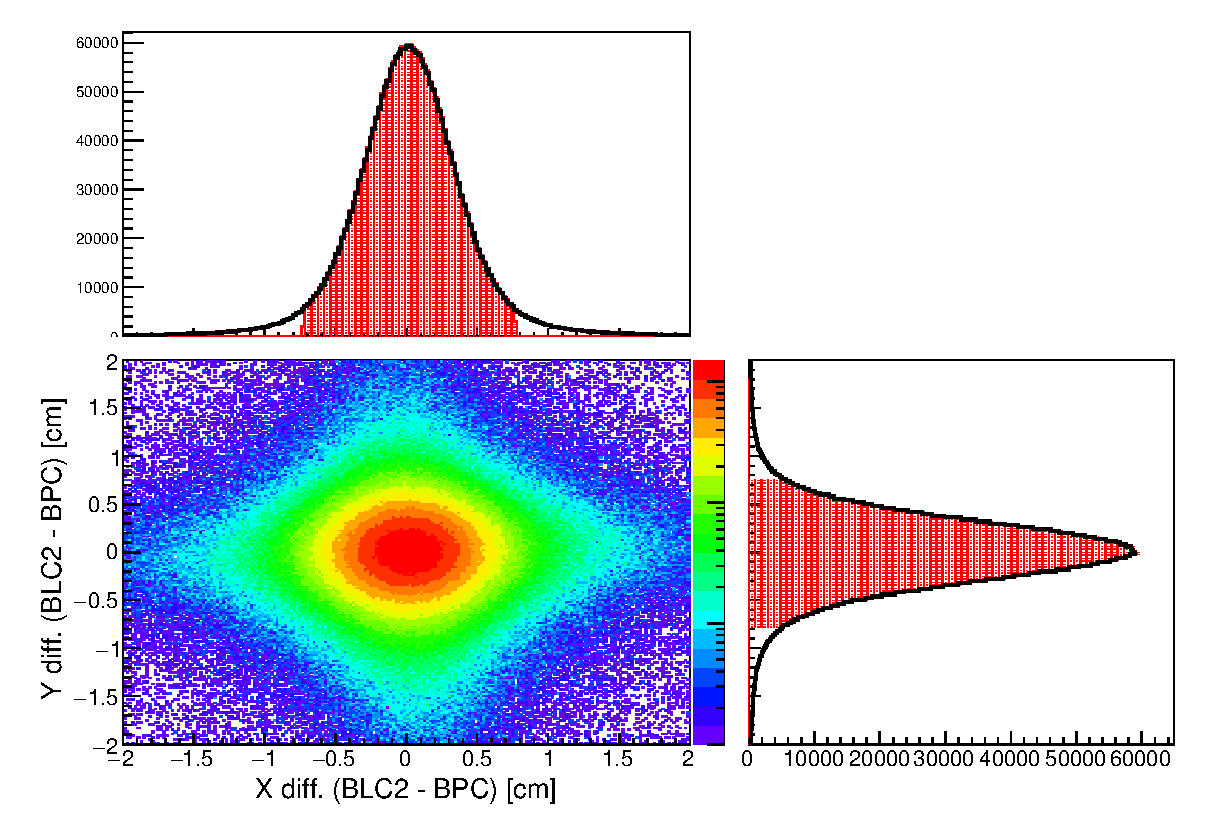
\includegraphics[width=6cm]{../pic/Run78/BL/BLC2BPC.eps}
    \end{minipage}
    \begin{minipage}{0.5\hsize}
      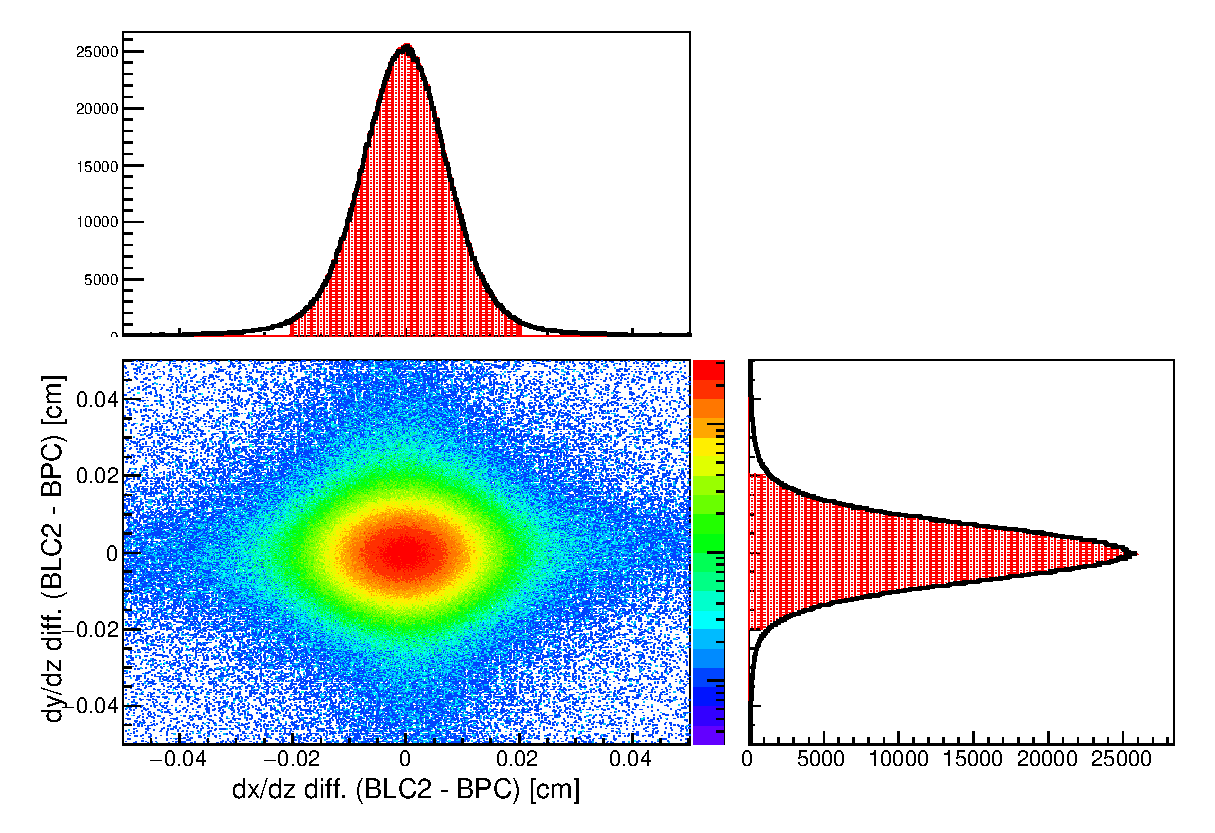
\includegraphics[width=6cm]{../pic/Run78/BL/BLC2BPC_dir.eps}
    \end{minipage}
  \end{tabular}
  \caption{
    These figures indicate the connection between the BLC2 and the BPC.
    The left figure shows about position matching at the center of these.
    The right figure shows direction matching.
    The red hatched region indicated an acceptable region.
  }
  \label{fig:BLC2BPC}
\end{figure}

\begin{figure}[htpb]
  \begin{tabular}{cc}
    \begin{minipage}{0.5\hsize}
      \includegraphics[width=6cm]{../pic/Run78/BL/profFF_Kf.eps}
    \end{minipage}
    \begin{minipage}{0.5\hsize}
      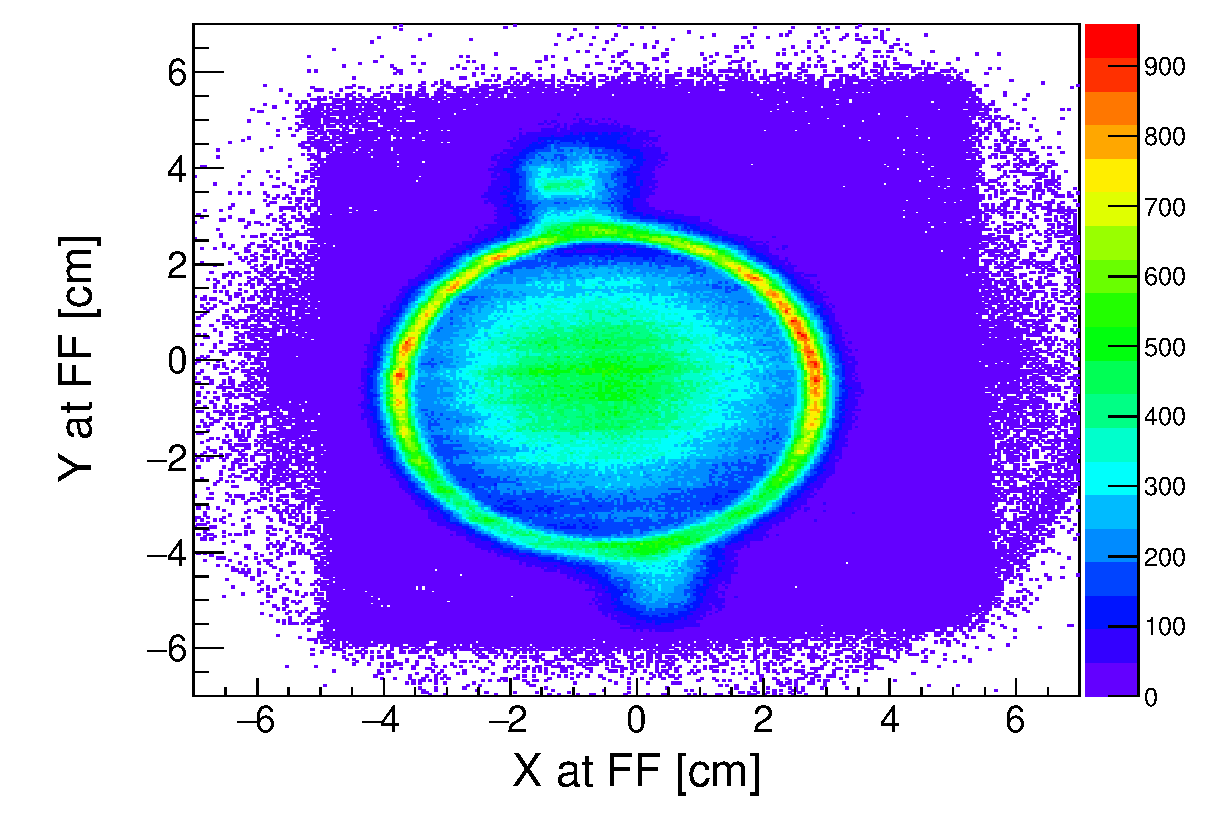
\includegraphics[width=6cm]{../pic/Run78/BL/profFF_KCDH2.eps}
    \end{minipage}
  \end{tabular}
  \caption{
    These figures shows beam profile at FF.
    The left figure shows about the unbiased kaon trigger.
    The right figure shows about CDH2 hit trigger.
  }
  \label{fig:profFF}
\end{figure}
The BPC is the same type drift chamber as BLC1/2, so the analysis of itself is the same as BLC1/2, which is shown in Fig\ref{fig:BLC_etc}.
There is no magnet between the BLC2 and the BPC, so trajectories reconstructed by them sshould be successfully connected within multiple scattering and resolution.
There are many materials between the BLC2 and the BPC, for example, the T0, the AC, BPD, and air, also direction ($dx/dz$ or $dy/dz$) resolution affects on extracted position resolution.
The $z$ length ratio of these is (BPC $z$)/(BLC2 $z$)=50.4mm/310mm$\sim$1/6, so extracted position resolution was almost decided by the BPC.
On the other hand, materials were placed at just down stream of the BLC2 for example the T0 and the AC.
These two effects were estimated almost the same, so we evaluated position matching at the center of the BLC2 and the BPC as Fig\ref{fig:BLC2BPC}.
We also require direction matching the right figure of Fig\ref{fig:BLC2BPC}.
The BPC also defines The beam profile at the experimental target position as shown in Fig\ref{fig:profFF}.
The profile required reaction at the trigger level was clearly seen target cell.
The red circle indicates an acceptable region as an effective kaon beam. %% todo Fiducialの赤枠

\begin{frame}{Profile at Final Forcus}
  \begin{tabular}{cc}
    \begin{minipage}{0.5\hsize}
      \begin{figure}
        Unbaised Kaon Trig.\\
        \includegraphics[width=6cm]{../pic/Run78/BL/profFF_Kf.eps}
      \end{figure}
    \end{minipage}

    \begin{minipage}{0.5\hsize}
      \begin{figure}
        CDH2 Trig.\\
        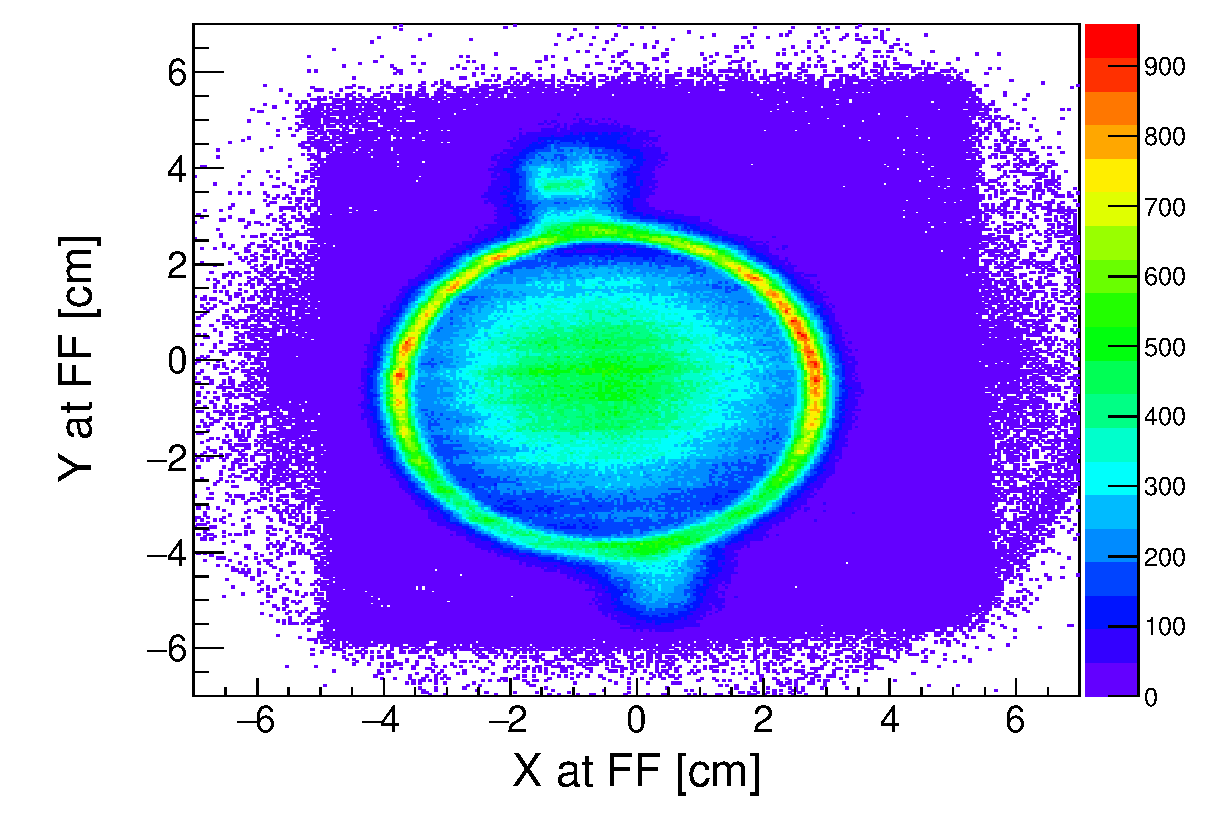
\includegraphics[width=6cm]{../pic/Run78/BL/profFF_KCDH2.eps}
      \end{figure}
    \end{minipage}
  \end{tabular}
\end{frame}



\begin{frame}
  \label{page:CDS}
  { \Huge CDS Analysis }
\end{frame}
\begin{frame}{CDC fine turning}
  \begin{tabular}{cc}
    \begin{minipage}{0.5\hsize}
      \begin{figure}
        Before\\
        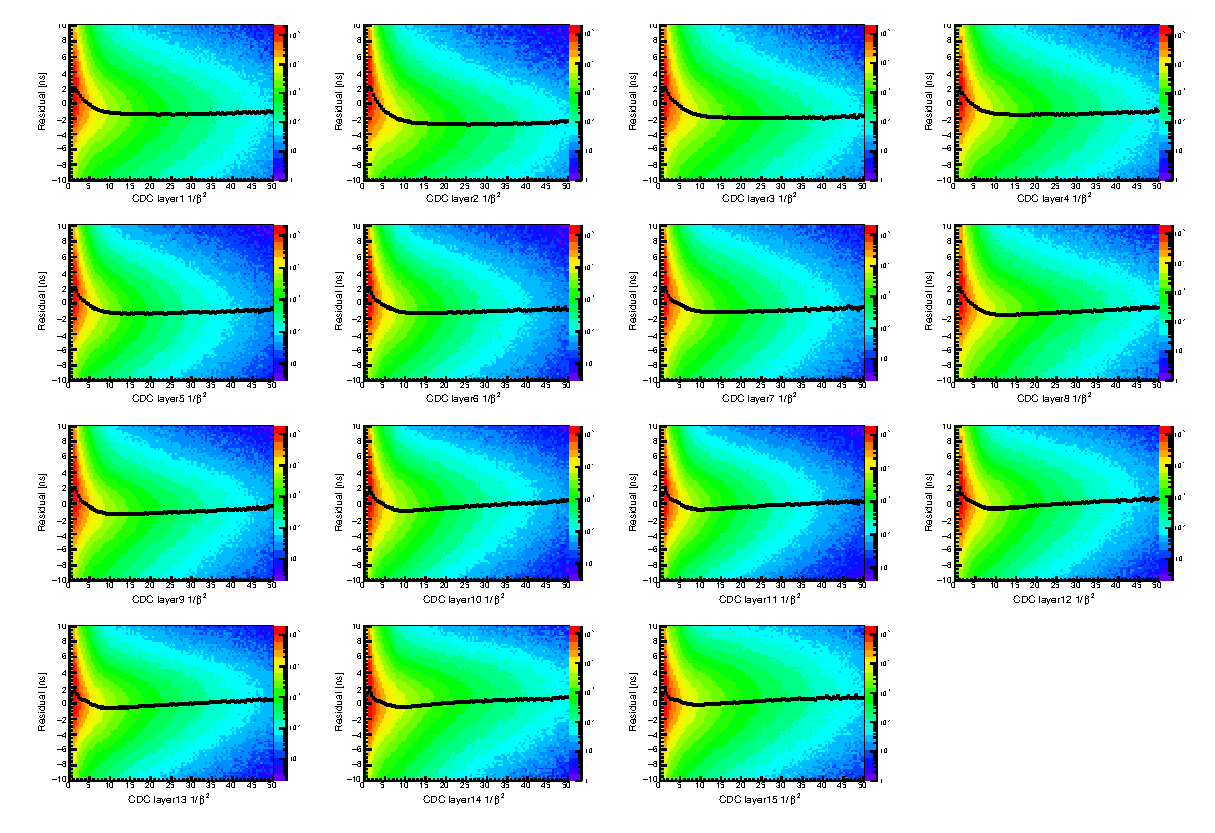
\includegraphics[width=5cm]{../pic/Run78/CDS/CDC_ob2_res_before.eps}
      \end{figure}
    \end{minipage}

    \begin{minipage}{0.5\hsize}
      \begin{figure}
        After\\
        \includegraphics[width=5cm]{../pic/Run78/CDS/CDC_ob2_res.eps}
      \end{figure}
    \end{minipage}
  \end{tabular}
  \centering
  $\beta$ and residual has correlation, which was calibrated wire-by-wire.
\end{frame}

\begin{frame}{Vertex image by CDS and BPC}
  \begin{figure}
    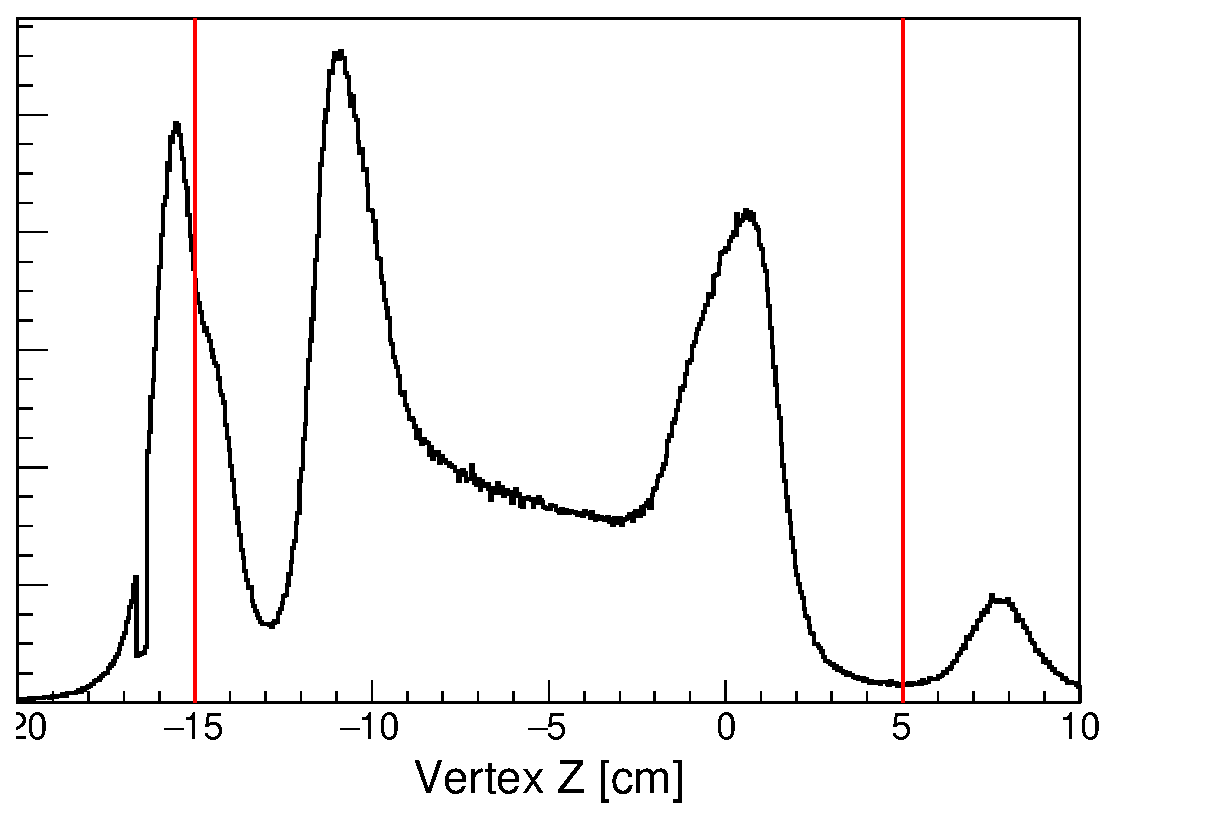
\includegraphics[width=8cm]{../pic/Run78/CDS/vertex.eps}
  \end{figure}
\end{frame}

\begin{frame}{Vertex image by CDS and BPC (Vertex cut)}
  \begin{figure}
    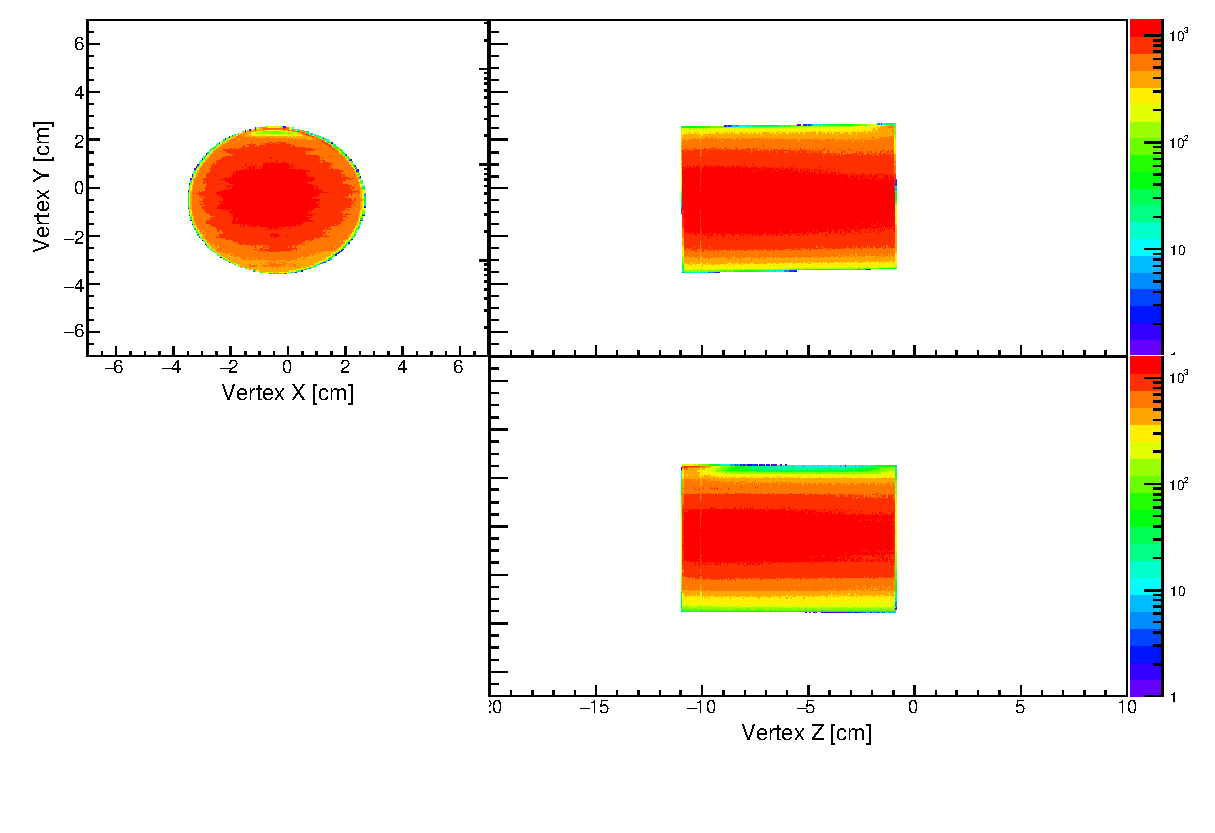
\includegraphics[width=8cm]{../pic/Run78/CDS/vertex_f.eps}
  \end{figure}
\end{frame}

\begin{frame}{Vertex resolution}
  \begin{tabular}{cc}
    \begin{minipage}{0.5\hsize}
      \begin{figure}
        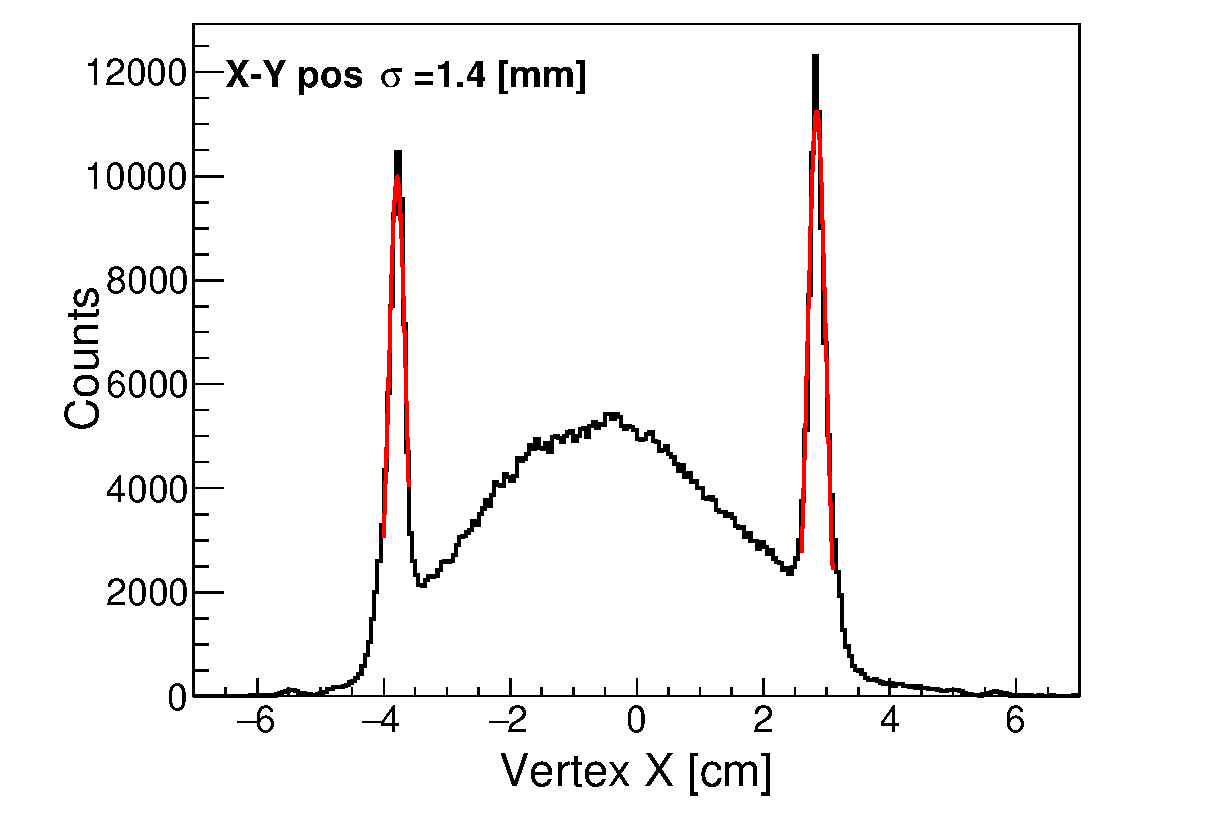
\includegraphics[width=5cm]{../pic/Run78/CDS/vertex_x.eps}
      \end{figure}
      \centering
      Y range was selected \\ $-5.5\sim-5$ [mm]
    \end{minipage}

    \begin{minipage}{0.5\hsize}
      \begin{figure}
        \includegraphics[width=5cm]{../pic/Run78/CDS/vertex_z.eps}
      \end{figure}
      \centering
      $Z =0$ was selected [mm]\\
      resolution was evaluated by DEF.
    \end{minipage}
  \end{tabular}
\end{frame}

\begin{frame}{CDS mass$^2$ vs momentum}
  \begin{figure}
    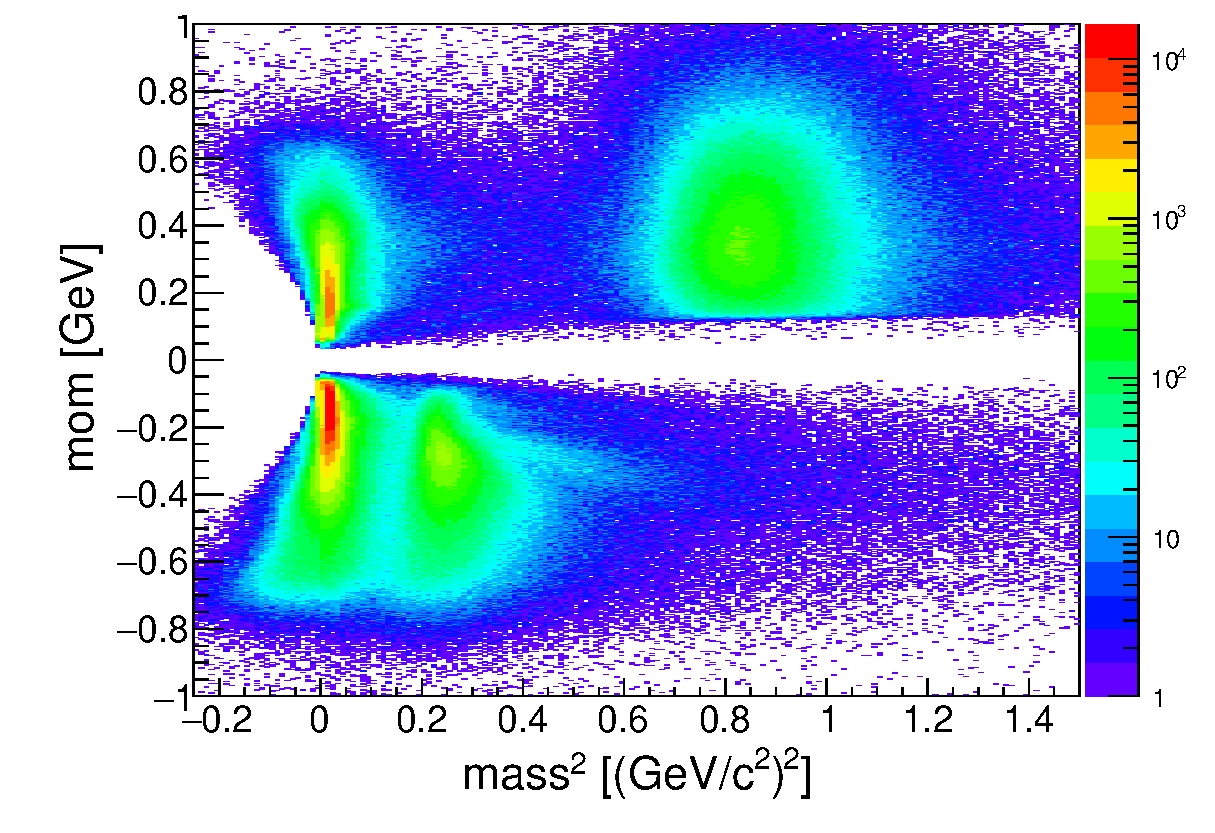
\includegraphics[width=8cm]{../pic/Run78/CDS/pid.eps}
  \end{figure}
\end{frame}

\begin{frame}{Invaraint mass by CDS}
  \begin{tabular}{cc}
    \begin{minipage}{0.5\hsize}
      \begin{figure}
        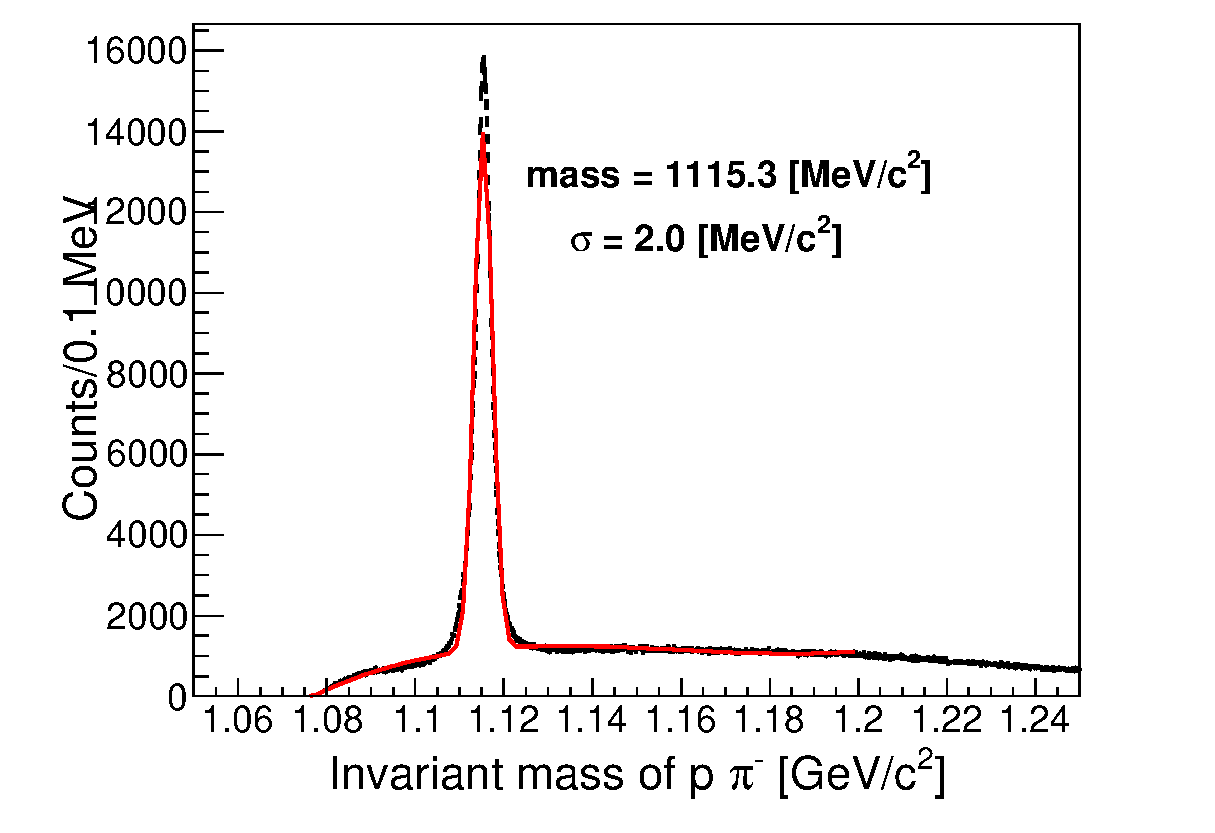
\includegraphics[width=5cm]{../pic/Run78/CDS/IM_ppim.eps}
      \end{figure}
    \end{minipage}

    \begin{minipage}{0.5\hsize}
      \begin{figure}
        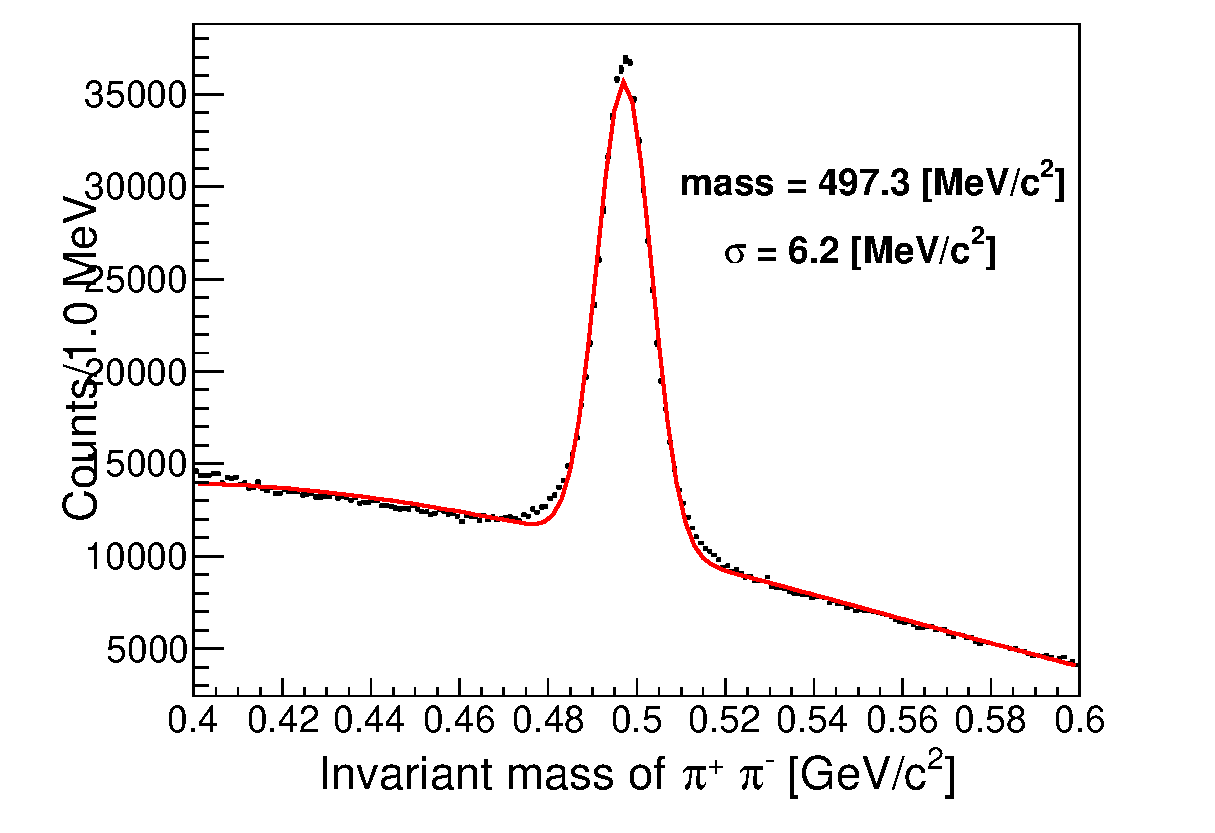
\includegraphics[width=5cm]{../pic/Run78/CDS/IM_pipi.eps}
      \end{figure}
    \end{minipage}
  \end{tabular}
\end{frame}




\begin{frame}
  \label{page:NC}
  { \Huge NC Analysis }
\end{frame}
\subsection{Neutron Counter - NC}
The neutron counter (NC) are located 14.7 m upstream of the target.
Because the NC are located at the most upstream and the purpose is to detecting neutral particles, the NC requires a large amount of material.
Therefore, the NC is a segmented scintillation detector with 7 layers, each layer consisting of 16 counters.
One scintillation detector is 20cm (width) $\times$ 150cm (height) $\times$ 5cm (thickness) in size.
So one layer covers 320cm (width) $\times$ 150cm (height), which is corresponds 6.2 degrees in horizontal and 2.9 degrees in vertical in this experiment setup.
The first three layers of the scintillator are made of Saint-Gobain BC408 and the other four layers are made of Saint-Gobain BC412.
The scintillation light is carried by lucite light guides on both sides and read out by the 2-inch PMT (Hamamatsu H6410).
Each layer is installed with a gap of 2 cm, so the whole NC has a thickness of 47 cm.
Differences between the upstream and downstream solid angles are evaluated as systematic errors.


\begin{frame}{$d(K^-, n)"\pi^{\pm}\Sigma^{\mp}"$ event selection}
  \begin{tabular}{cc}
    \begin{minipage}{0.5\hsize}
      { \scriptsize
        $d(K^-, n \pi^+ \pi^-)"n"$ was selected by 2$\sigma$.\\
        $K^- d \rightarrow K^0 n n $ was selected by 3$\sigma$.\\
        $K^- d \rightarrow \Sigma^{\pm}\pi^{\mp} n_{miss}$ was rejected by 3$\sigma$.
      }
      \begin{figure}
        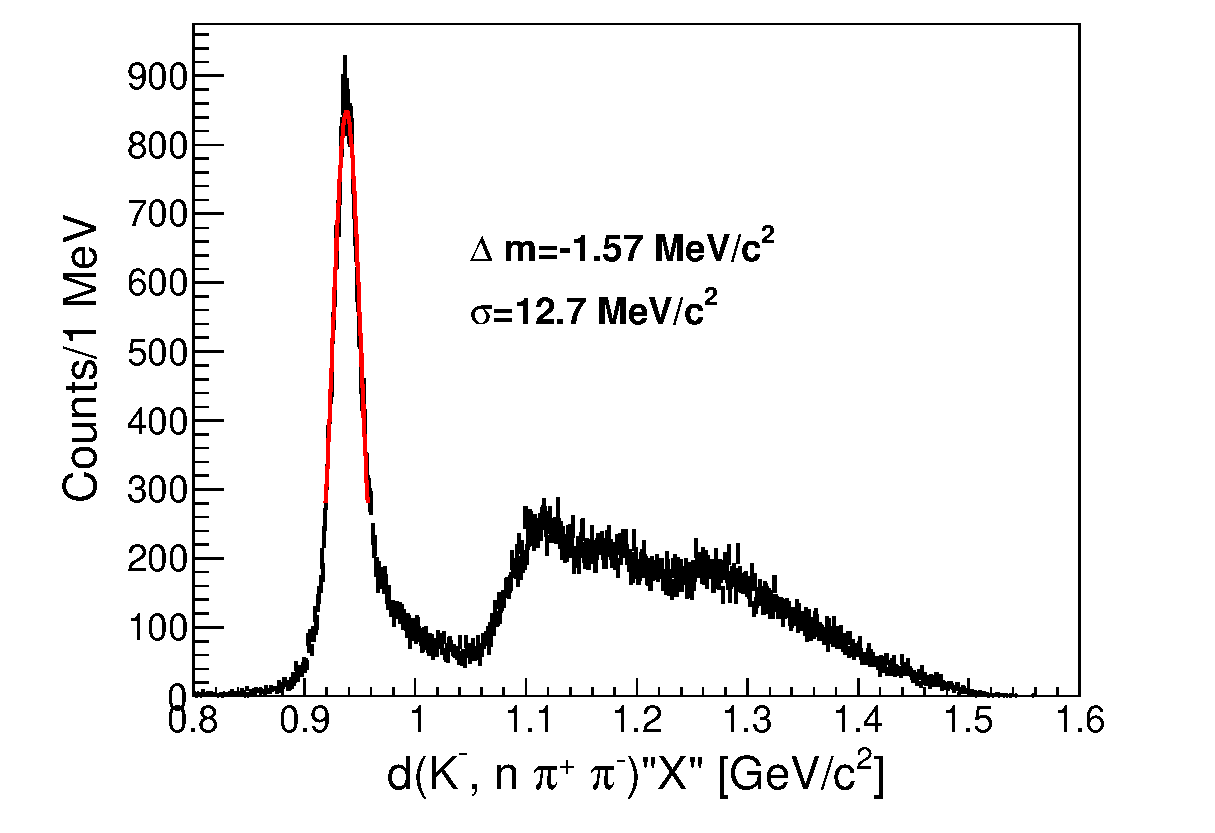
\includegraphics[width=5cm]{../pic/Run78/KN_ana_NC170_2sigma/KNpipi_MM_woFit.eps}
      \end{figure}
    \end{minipage}

    \begin{minipage}{0.5\hsize}
      \begin{figure}
        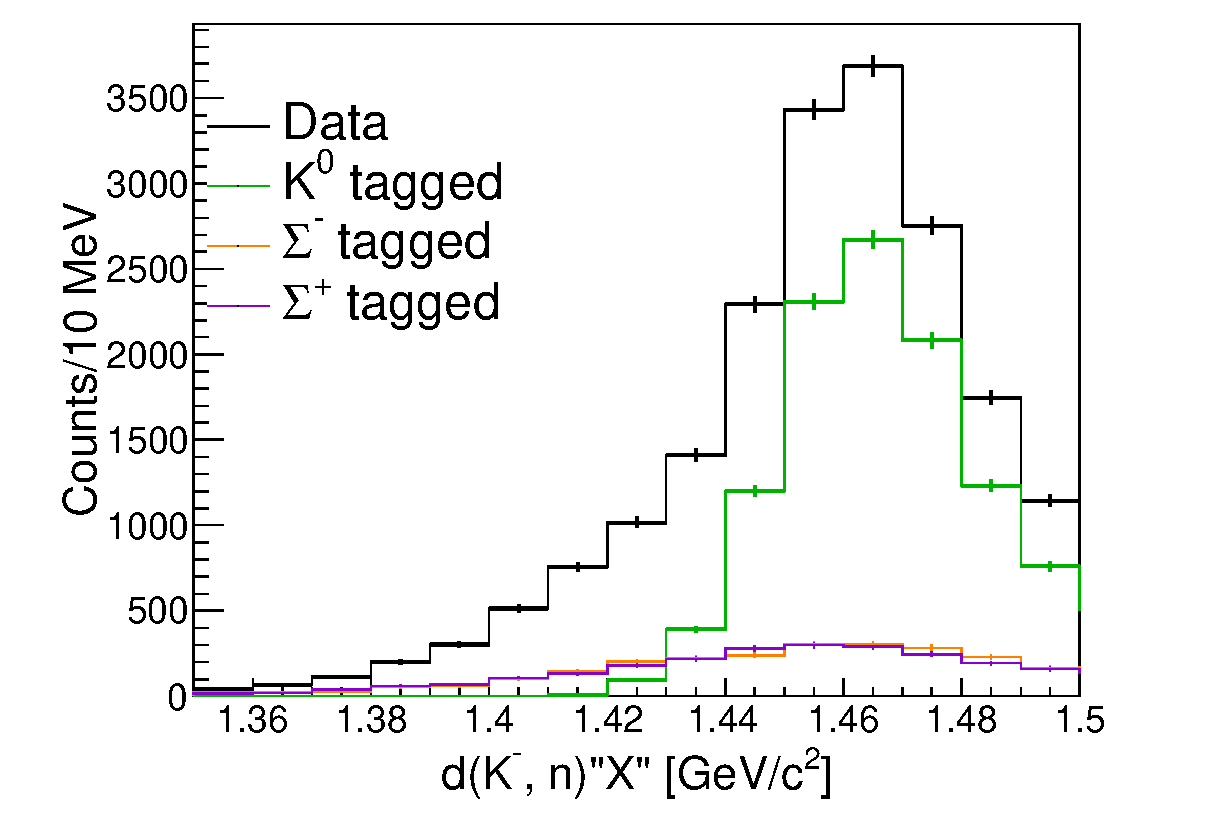
\includegraphics[width=6cm]{../pic/Run78/KN_ana_NC170_2sigma/KN_MM_all.eps}
      \end{figure}
    \end{minipage}
  \end{tabular}

  \begin{tabular}{cc}
    \begin{minipage}{0.33\hsize}
      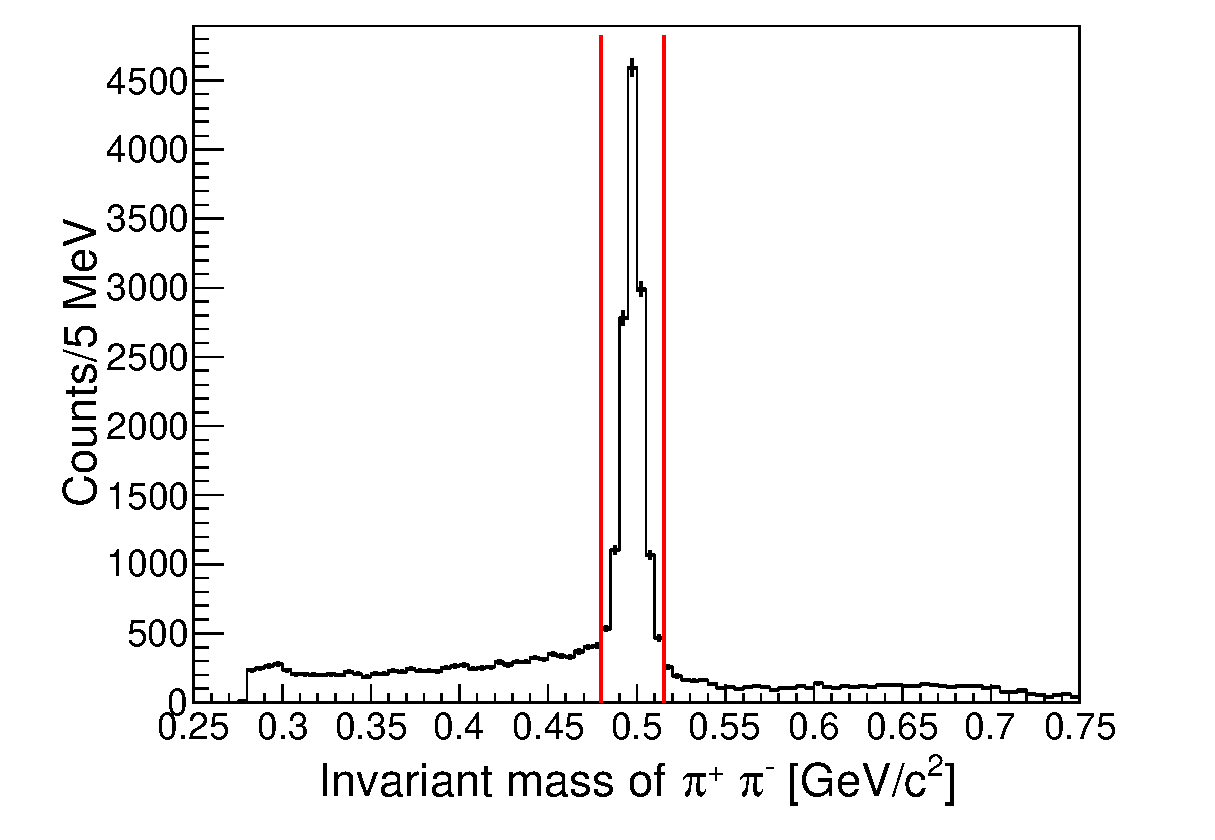
\includegraphics[width=3cm]{../pic/Run78/KN_ana_NC170_2sigma/IM_pipi_woFit.eps}
    \end{minipage}

    \begin{minipage}{0.33\hsize}
      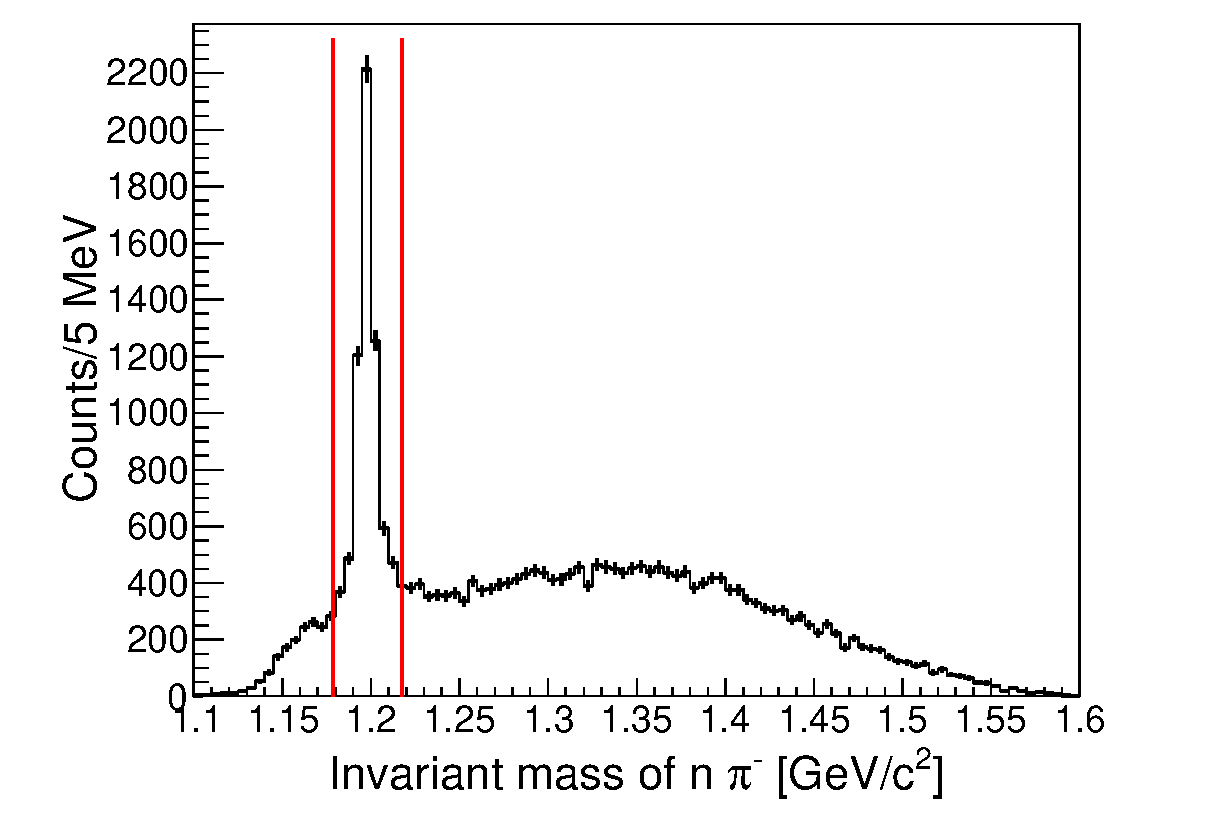
\includegraphics[width=3cm]{../pic/Run78/KN_ana_NC170_2sigma/IM_npim_woFit.eps}
    \end{minipage}

    \begin{minipage}{0.33\hsize}
      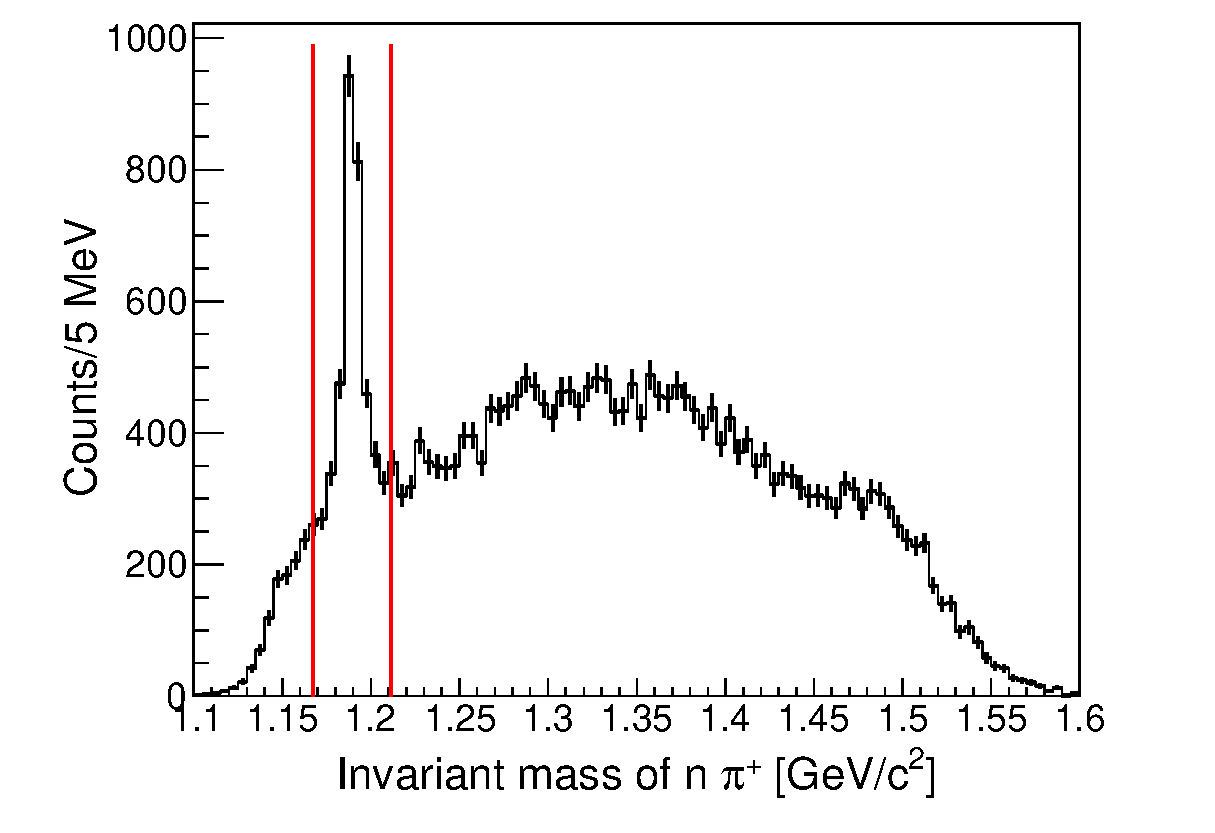
\includegraphics[width=3cm]{../pic/Run78/KN_ana_NC170_2sigma/IM_npip_woFit.eps}
    \end{minipage}
  \end{tabular}
\end{frame}


\begin{frame}{Reaction Identification}
  We expect these three reactions.
  \begin{itemize}
  \item $K^- d\rightarrow \pi^{\pm}"\Sigma^{\mp}" n_{forward}$ (Signal)
  \item $K^- d\rightarrow K^{0} n n$ (Quasi-elastic)
  \item $K^- d\rightarrow "n" \pi^{\pm} \Sigma^{\mp}_{forward}$ $\Sigma^{\mp}_{forward}\rightarrow n_{forward} \pi^{\mp}$
  \end{itemize}

  Identification method procedure.
  \begin{itemize}
  \item Three invariamt mass fitting of $\pi^+ \pi^-$, $n \pi^{\pm}$.\\
    $\rightarrow$ In this fitting, $K^- d\rightarrow \pi^{\pm}"\Sigma^{\mp}" n_{forward}$ was fixed.
    
  \item Missing mass of $d(K^-, n \pi^{\pm})"\Sigma^{\mp}"$ fitting.\\
    $\rightarrow$ In this fitting, $K^- d\rightarrow K^{0} n n$, $K^- d\rightarrow "n" \pi^{\pm} \Sigma^{\mp}_{forward}$ were fixed. \\
    $\rightarrow$ This fitting was performed bin-by-bin of $d(K^-, n)"X"$.\\
  \item These fitting was performed iterationary.
  \end{itemize}

  Fitting method was adopted below method.\\
  { \tiny
    \href{https://www.sciencedirect.com/science/article/pii/001046559390005W}{R. Barlow and C. Beeston, Comp. Phys. Comm. 77 (1993) 219-228 \\ \vspace{-3mm}
      "Fitting using finite Monte Carlo samples"}
  }
  
  { \tiny
    \href{https://www.sciencedirect.com/science/article/pii/S0010465508003652}{A.Nappi, Comp Phys. Comm. 180 (2009) 269-275 \\ \vspace{-3mm}
      "A pitfall in the use of extended likelihood for fitting fractions of pure samples in a mixed sample"}
  }
\end{frame}


\begin{frame}{$d(K^-, n \pi^+ \pi^-)"X"$ data and MC (NC $\sigma=150ps$)}
  \begin{itemize}
  \item $K^- d\rightarrow (\pi^{\pm}\Sigma^{\mp})_{backwoard} n_{forward}$ (Signal)
  \item $K^- d\rightarrow K^{0} n n$ (Quasi-elastic)
  \item $K^- d\rightarrow n \pi^{\pm} \Sigma^{\mp}_{forward}$ 

  \end{itemize}
  \begin{tabular}{cc}
    \begin{minipage}{0.6\hsize}
      \begin{figure}
        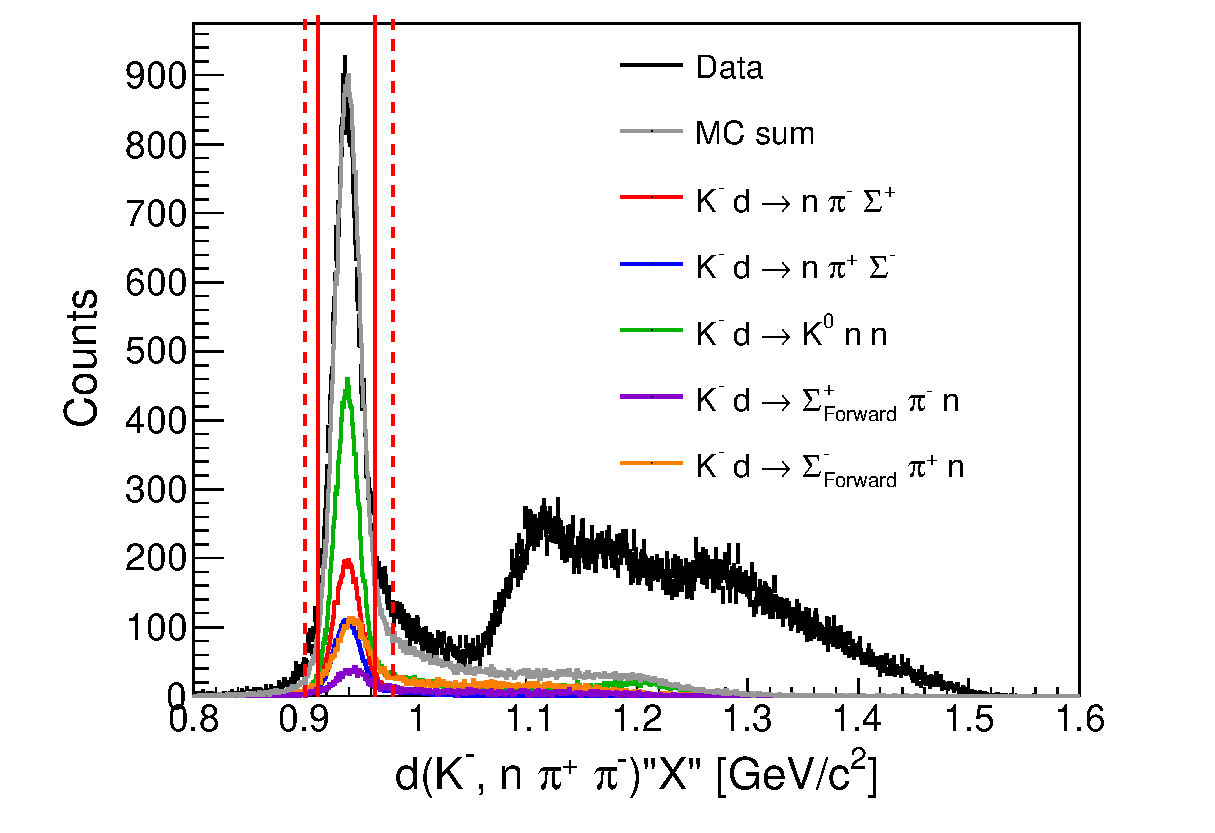
\includegraphics[width=6cm]{../pic/Run78/KN_ana_3sigma/fitKNpipi_MM.eps}
      \end{figure}
    \end{minipage}
    \begin{minipage}{0.4\hsize}
      \begin{figure}
        Data fitting\\
        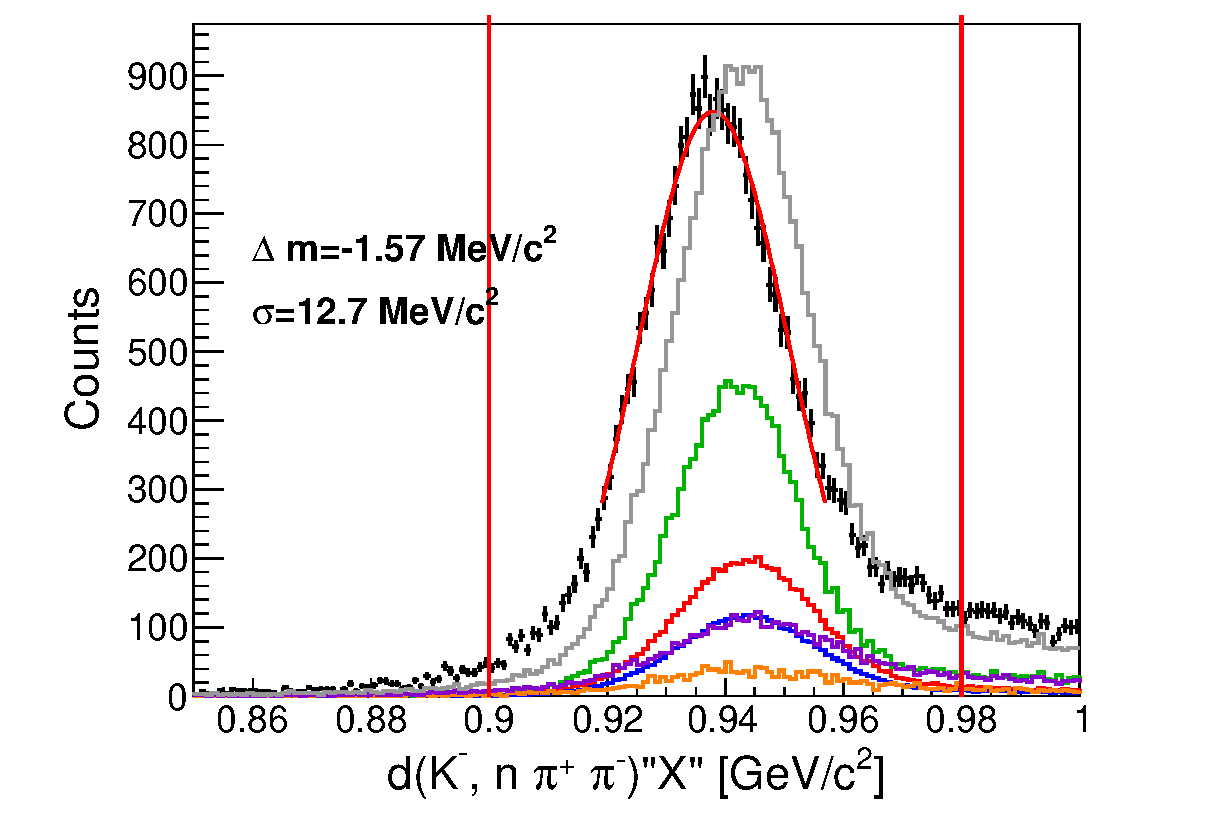
\includegraphics[width=3cm]{../pic/Run78/KN_ana_3sigma/fitKNpipi_MM_fitData.eps}\\
        MC fitting\\
        \includegraphics[width=3cm]{../pic/Run78/KN_ana_3sigma/fitKNpipi_MM_fitMC.eps}
      \end{figure}
    \end{minipage}
  \end{tabular}
\end{frame}
 
\begin{frame}{Invaraint mass by CDS}
  \begin{tabular}{cc}
    \begin{minipage}{0.5\hsize}
      \begin{figure}
        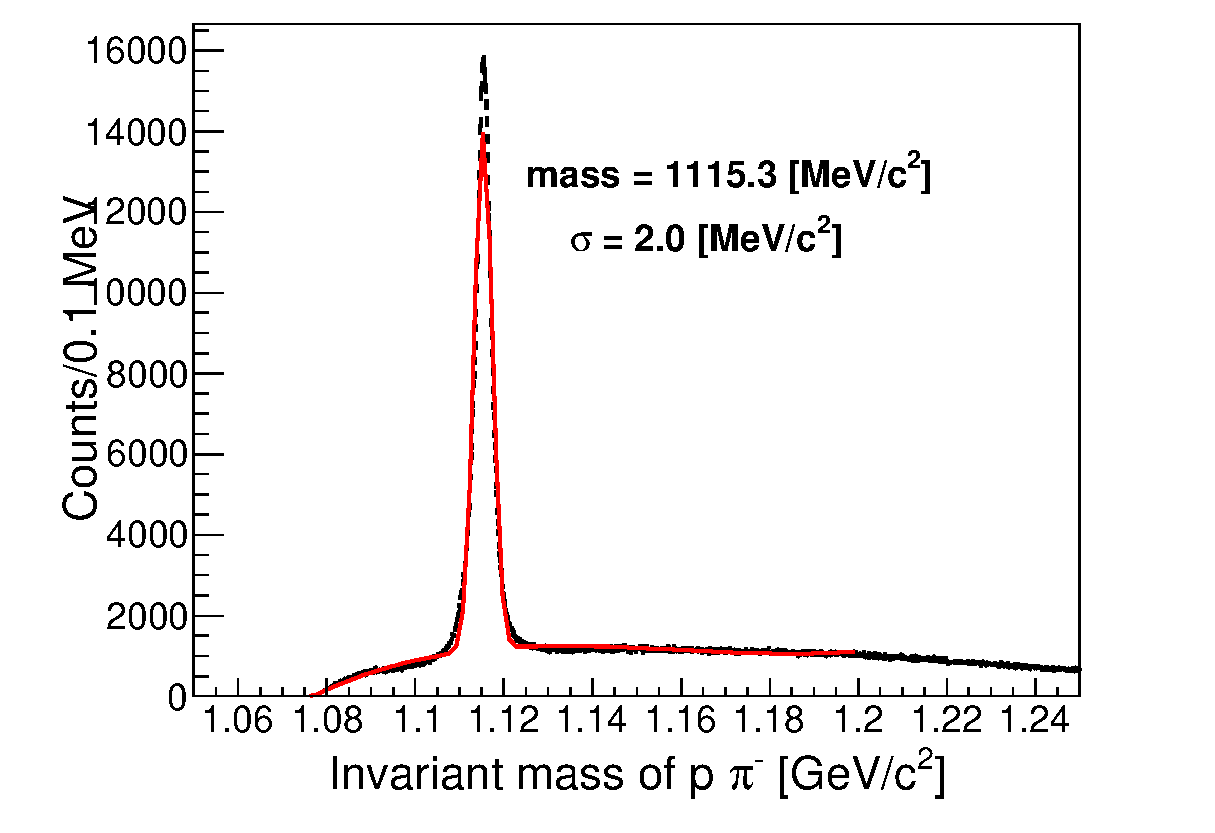
\includegraphics[width=5cm]{../pic/Run78/CDS/IM_ppim.eps}
      \end{figure}
    \end{minipage}

    \begin{minipage}{0.5\hsize}
      \begin{figure}
        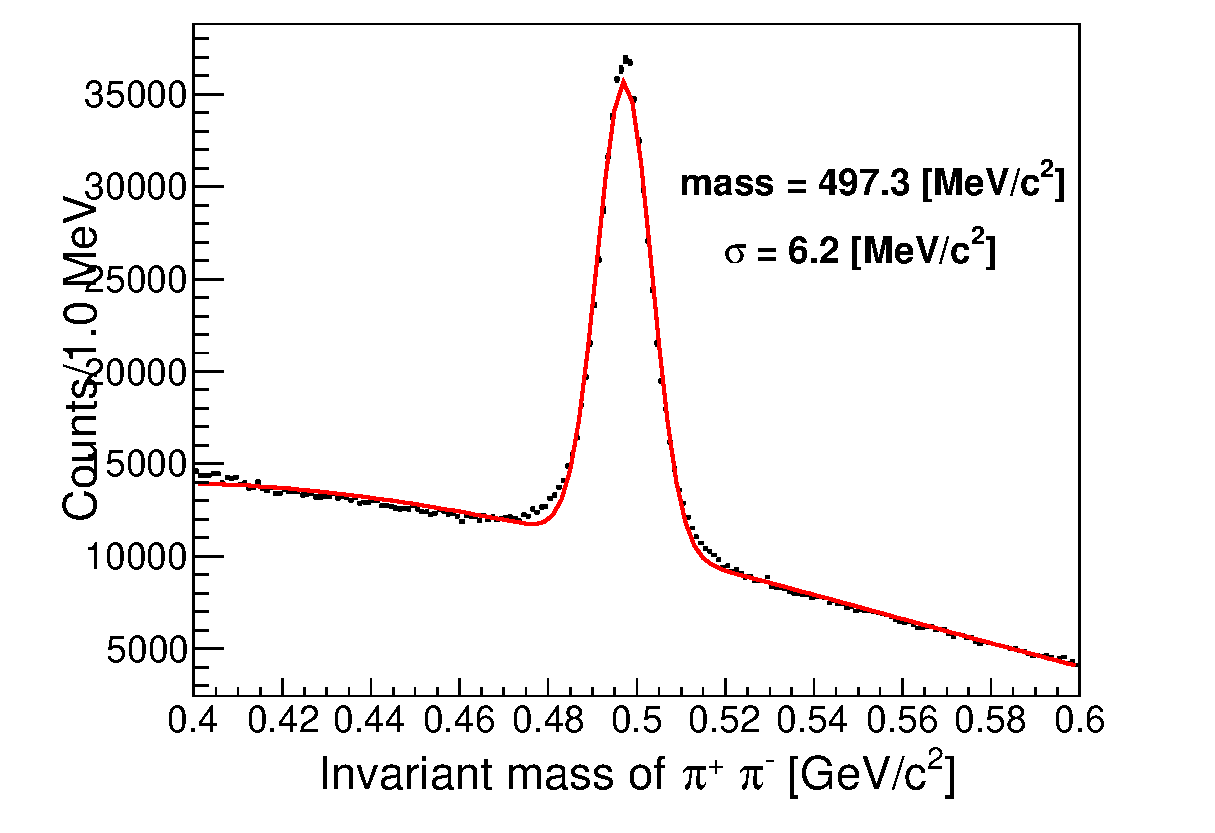
\includegraphics[width=5cm]{../pic/Run78/CDS/IM_pipi.eps}
      \end{figure}
    \end{minipage}
  \end{tabular}
\end{frame}

\begin{frame}{Template Fittig (All result summed) (NC $\sigma=170ps$)}
  $\pi^-\Sigma^+$ and $\pi^+ \Sigma^-$ modes were separated by fitting of $d(K^-, n \pi^{\pm})"\Sigma^{\mp}"$ .\\
  This fitting was performed bin-by-bin.
  
  \begin{figure}
    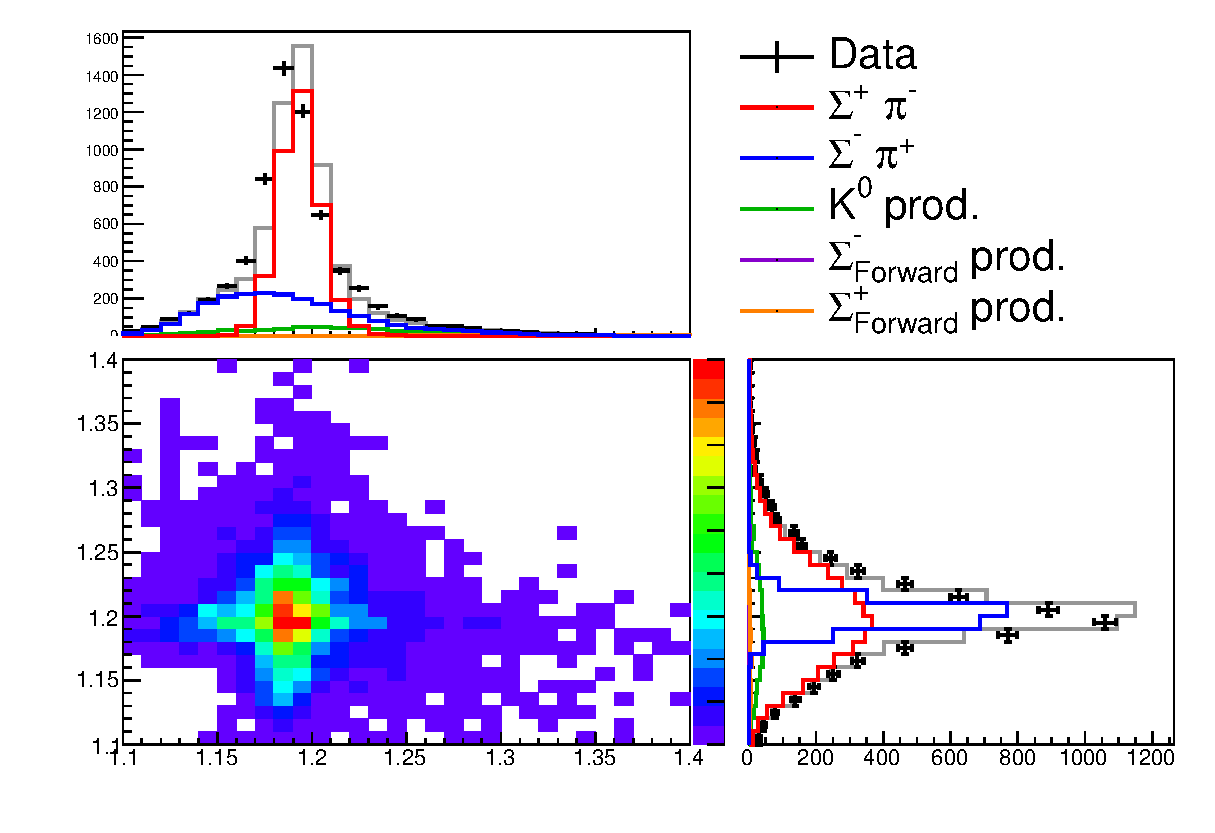
\includegraphics[width=6cm]{../pic/Run78/KN_ana_NC170_2sigma/KNpim_KNpip_MM.eps}
  \end{figure}
\end{frame}

\begin{frame}{$d(K^-, n \pi)"\Sigma"$ Fitting (NC $\sigma=150ps$)}
  \begin{tabular}{cc}
    \begin{minipage}{0.5\hsize}
      \begin{figure}
        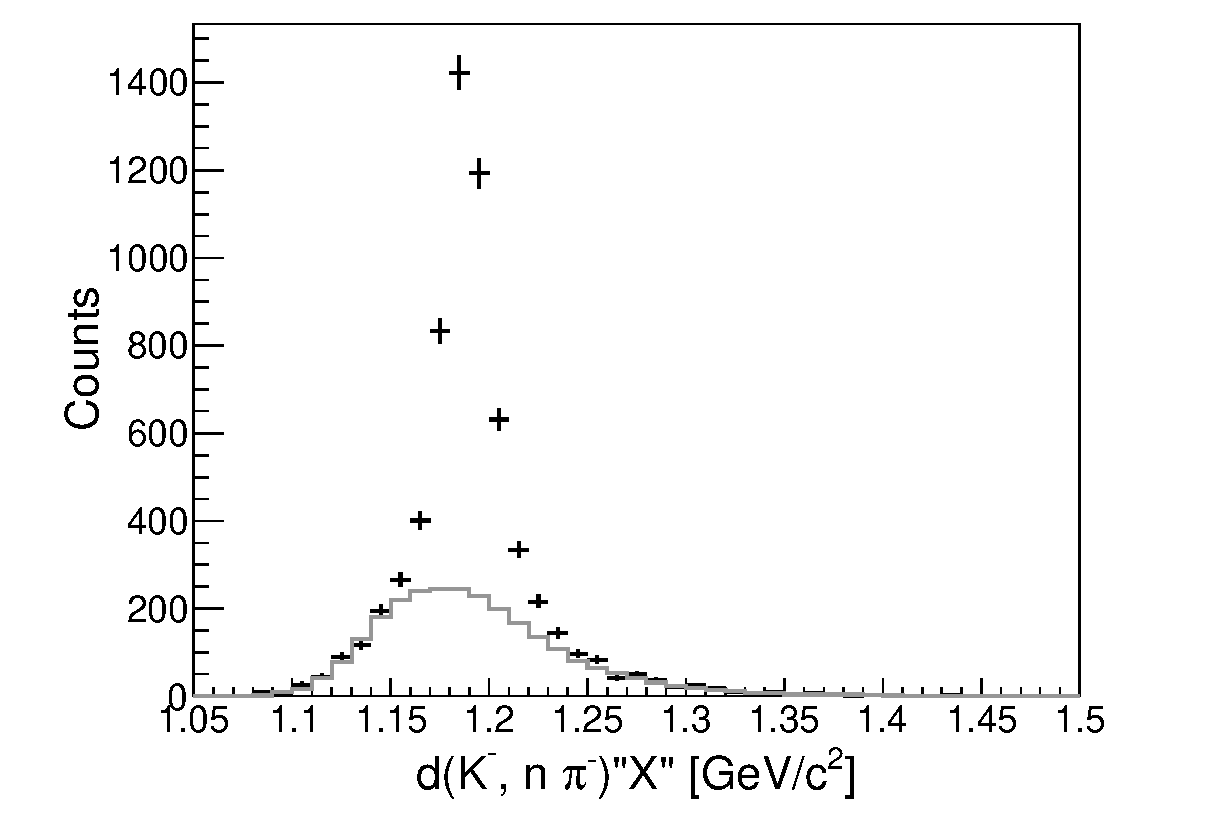
\includegraphics[width=3cm]{../pic/Run78/KN_ana_3sigma/fitKNpim_MM_data_wBG.eps}
      \end{figure}
    \end{minipage}

    \begin{minipage}{0.5\hsize}
      \begin{figure}
        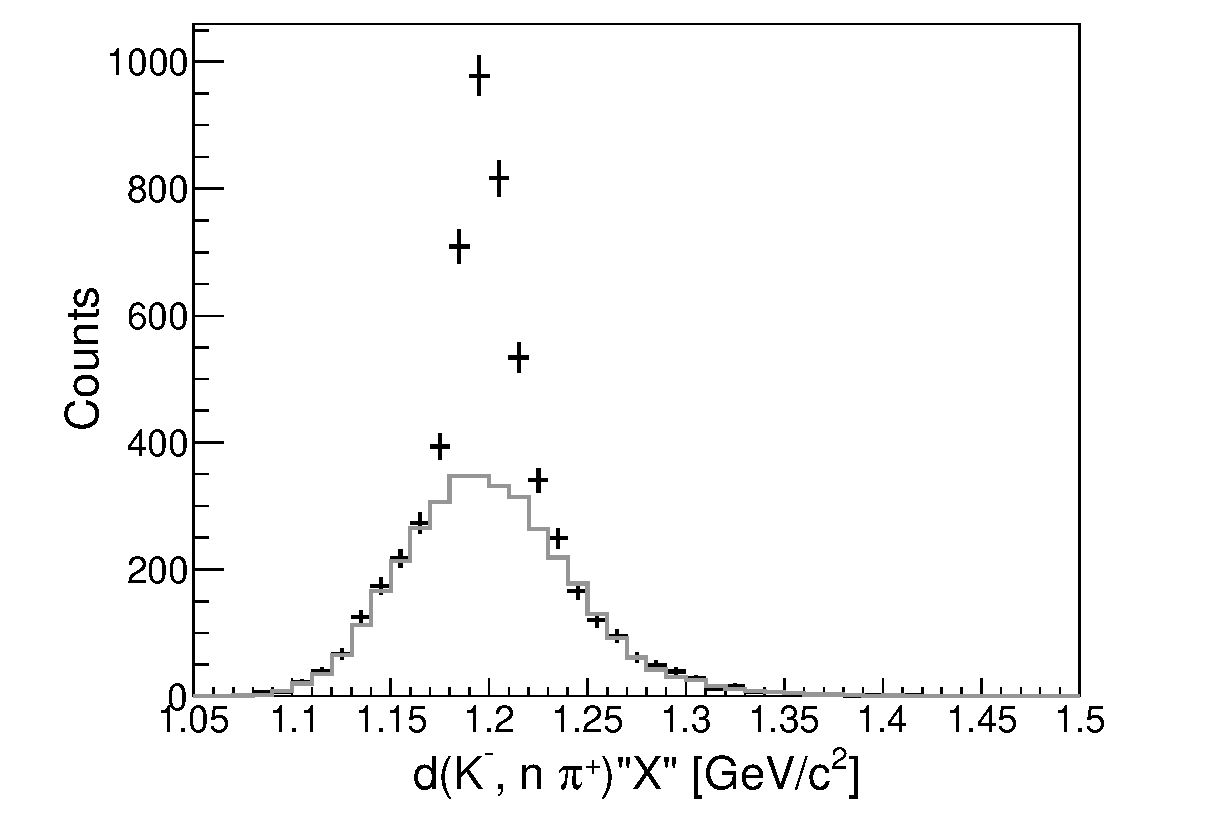
\includegraphics[width=3cm]{../pic/Run78/KN_ana_3sigma/fitKNpip_MM_data_wBG.eps}
      \end{figure}
    \end{minipage}
  \end{tabular}

  \begin{tabular}{cc}
    \begin{minipage}{0.5\hsize}
      \begin{figure}
        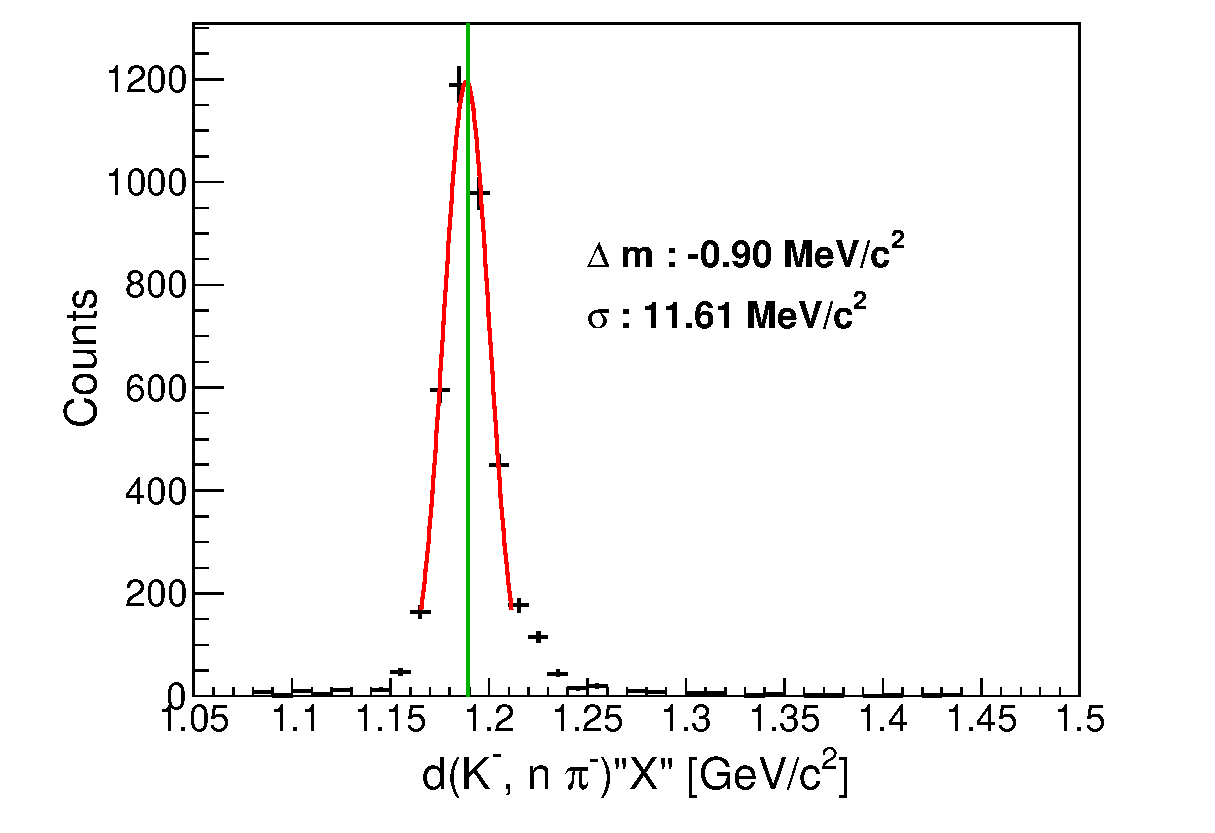
\includegraphics[width=3cm]{../pic/Run78/KN_ana_3sigma/fitKNpim_MM_data.eps}
      \end{figure}
    \end{minipage}

    \begin{minipage}{0.5\hsize}
      \begin{figure}
        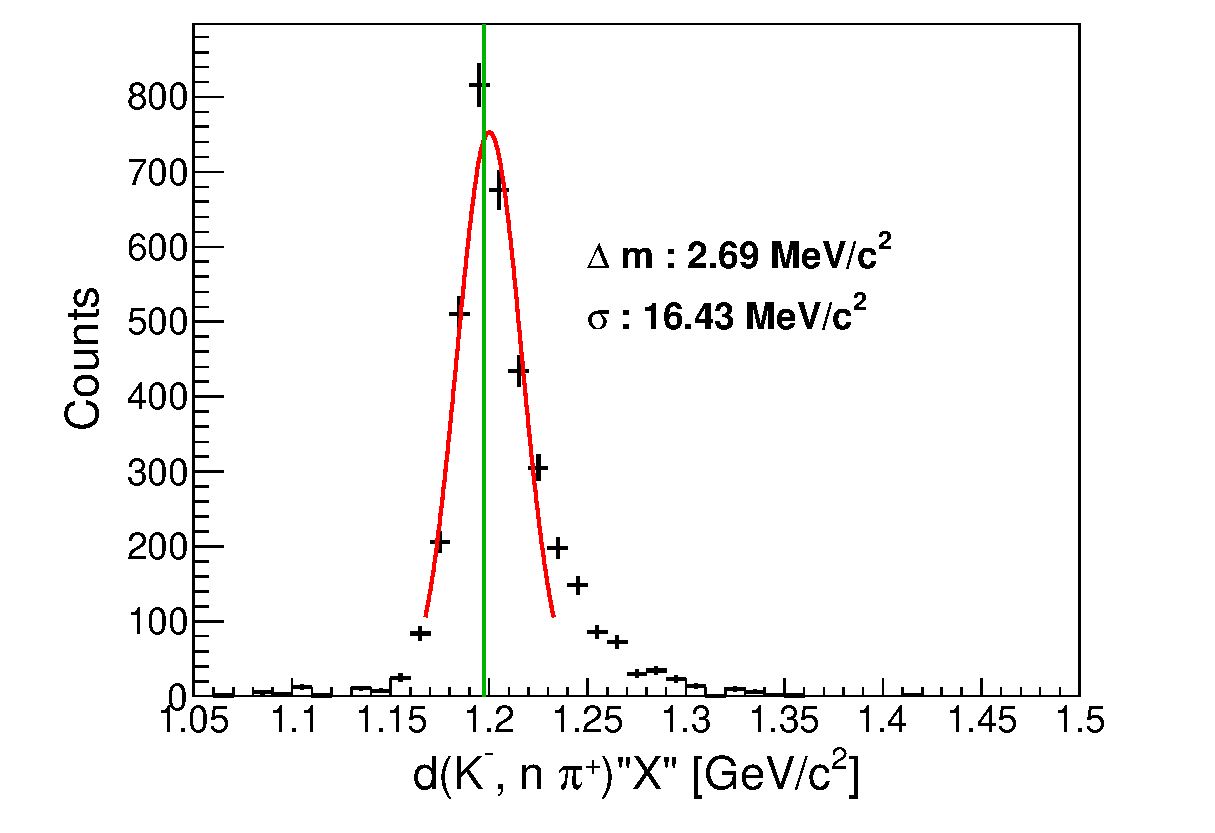
\includegraphics[width=3cm]{../pic/Run78/KN_ana_3sigma/fitKNpip_MM_data.eps}
      \end{figure}
    \end{minipage}
  \end{tabular}

  \begin{tabular}{cc}
    \begin{minipage}{0.5\hsize}
      \begin{figure}
        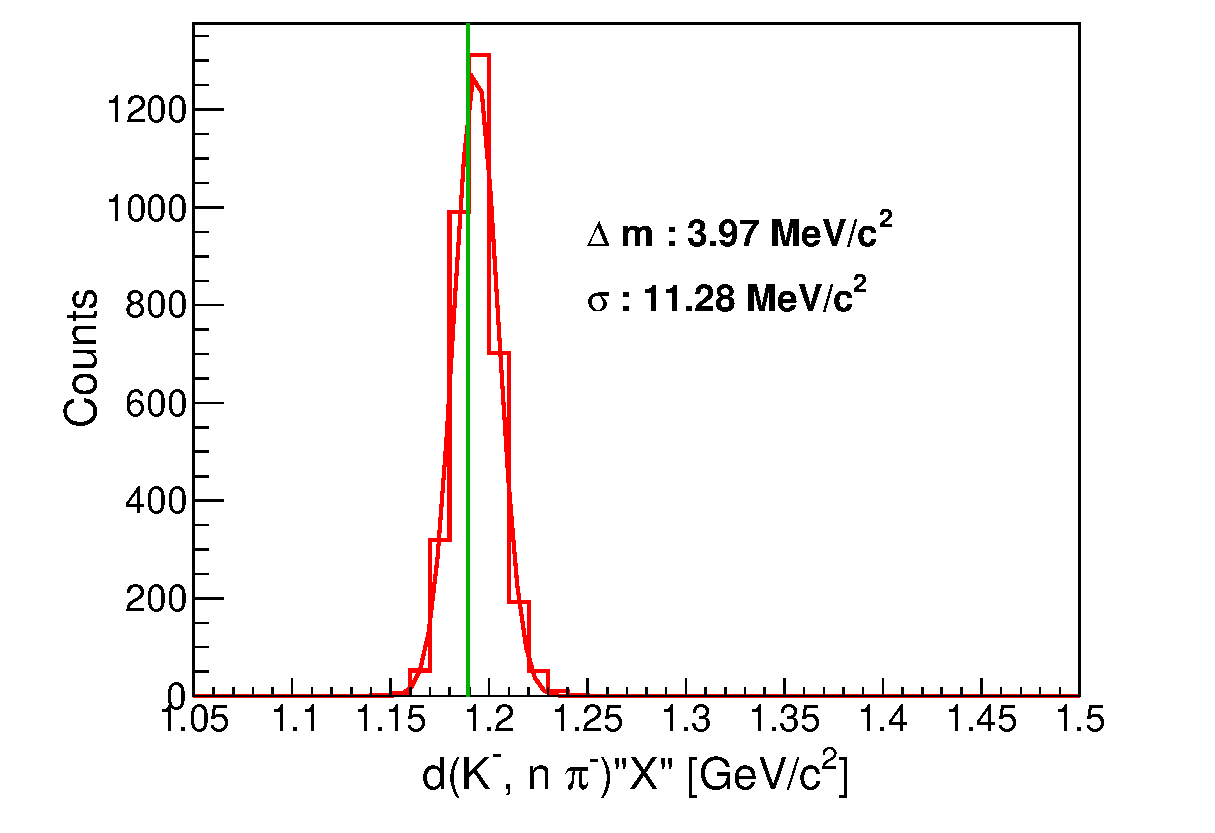
\includegraphics[width=3cm]{../pic/Run78/KN_ana_3sigma/fitKNpim_MM_MC.eps}
      \end{figure}
    \end{minipage}

    \begin{minipage}{0.5\hsize}
      \begin{figure}
        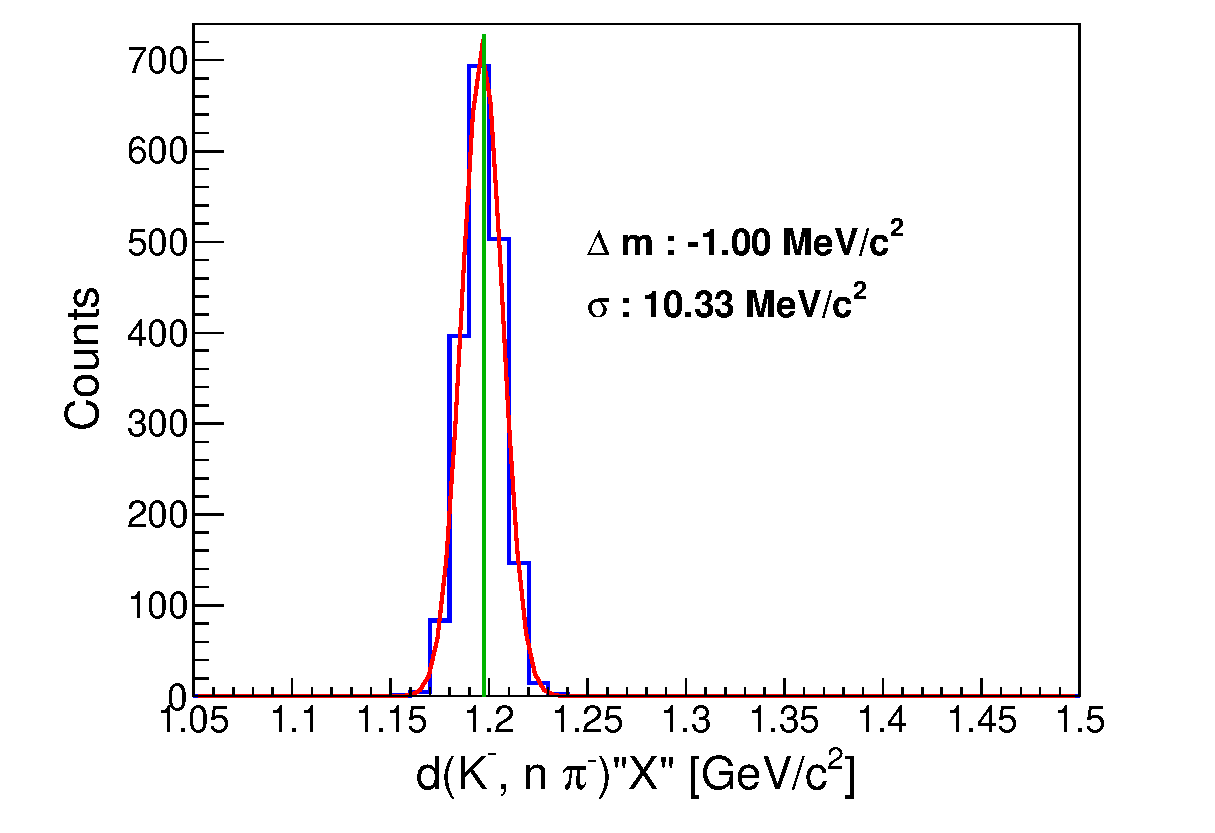
\includegraphics[width=3cm]{../pic/Run78/KN_ana_3sigma/fitKNpip_MM_MC.eps}
      \end{figure}
    \end{minipage}
  \end{tabular}
\end{frame}

\begin{frame}{$\ln(\Lambda)$}
  \begin{figure}
    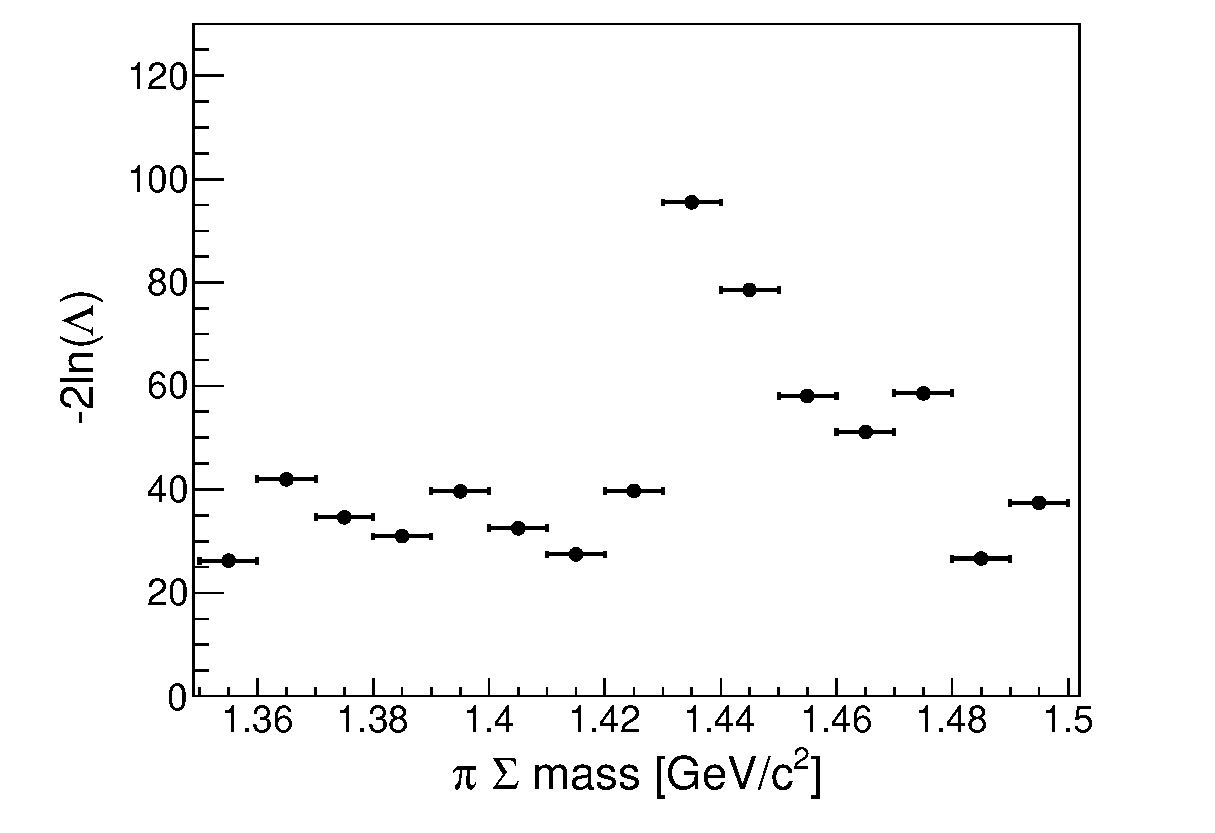
\includegraphics[width=10cm]{../pic/Run78/KN_ana_NC170_25sigma/Chi2.eps}
  \end{figure}
\end{frame}

\begin{frame}{Separated $\pi^{\pm}\Sigma^{\mp}$ Number}
  \begin{figure}
    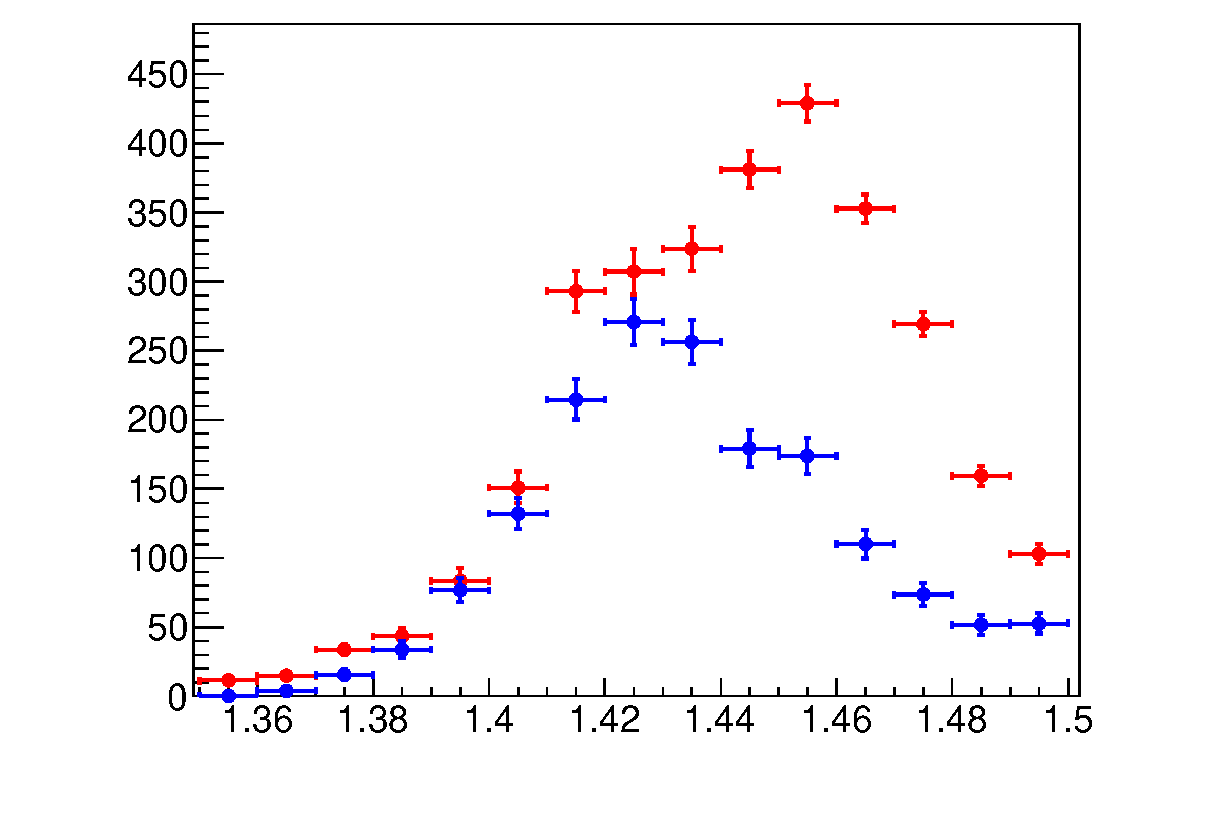
\includegraphics[width=8cm]{../pic/Run78/KN_ana_3sigma/piS_num.eps}
  \end{figure}
\end{frame}

\begin{frame}{Acceptance of $\pi^{\pm}\Sigma^{\mp}$}
  \begin{figure}
    \includegraphics[width=8cm]{../pic/Run78/KN_ana_3sigma/kn_acc.eps}
  \end{figure}
\end{frame}

\begin{frame}{$\pi^{\pm}\Sigma^{\mp}$ Cross Section}
  \begin{figure}
    \includegraphics[width=7cm]{../pic/Run78/KN_ana_3sigma/pimSp_pipSm_CS.eps}
  \end{figure}
\end{frame}

\begin{frame}{$\pi^{\pm}\Sigma^{\mp}$ Average Cross Section}
  \begin{figure}
    \includegraphics[width=7cm]{../pic/Run78/KN_ana_3sigma/Charge_ave_CS.eps}
  \end{figure}
\end{frame}

%% \input{KN_ana_NC170_2sigma/KNpi_MM/KNpi_MM_0}
\input{KN_ana_NC170_2sigma/KNpi_MM/KNpi_MM_1}
\input{KN_ana_NC170_2sigma/KNpi_MM/KNpi_MM_2}
\input{KN_ana_NC170_2sigma/KNpi_MM/KNpi_MM_3}
\input{KN_ana_NC170_2sigma/KNpi_MM/KNpi_MM_4}
\input{KN_ana_NC170_2sigma/KNpi_MM/KNpi_MM_5}
\input{KN_ana_NC170_2sigma/KNpi_MM/KNpi_MM_6}
\input{KN_ana_NC170_2sigma/KNpi_MM/KNpi_MM_7}
\input{KN_ana_NC170_2sigma/KNpi_MM/KNpi_MM_8}
\input{KN_ana_NC170_2sigma/KNpi_MM/KNpi_MM_9}
\input{KN_ana_NC170_2sigma/KNpi_MM/KNpi_MM_10}
\input{KN_ana_NC170_2sigma/KNpi_MM/KNpi_MM_11}
\input{KN_ana_NC170_2sigma/KNpi_MM/KNpi_MM_12}
\input{KN_ana_NC170_2sigma/KNpi_MM/KNpi_MM_13}
\input{KN_ana_NC170_2sigma/KNpi_MM/KNpi_MM_14}
\input{KN_ana_NC170_2sigma/KNpi_MM/KNpi_MM_15}
\input{KN_ana_NC170_2sigma/KNpi_MM/KNpi_MM_16}
\input{KN_ana_NC170_2sigma/KNpi_MM/KNpi_MM_17}
\input{KN_ana_NC170_2sigma/KNpi_MM/KNpi_MM_18}
\input{KN_ana_NC170_2sigma/KNpi_MM/KNpi_MM_19}
\input{KN_ana_NC170_2sigma/KNpi_MM/KNpi_MM_20}
\input{KN_ana_NC170_2sigma/KNpi_MM/KNpi_MM_21}
\input{KN_ana_NC170_2sigma/KNpi_MM/KNpi_MM_22}
\input{KN_ana_NC170_2sigma/KNpi_MM/KNpi_MM_23}
\input{KN_ana_NC170_2sigma/KNpi_MM/KNpi_MM_24}



%% \begin{frame}{Summary of error estimation}
  \begin{itemize}
  \item Difference of horizontal axis.
    $\rightarrow$ Estimation using $d(K^-, n \pi^+ \pi^-)"n"$, $d(K^-, n \pi^-)"\Sigma^+"$ and $d(K^-, n \pi^+)"\Sigma^-"$ peaks\\
    $\rightarrow$ Difference within 2$MeV/c^2$.
  \item Staticical error of $d(K^-, n \pi^+ \pi^-)"n"$ events.\\
    $\rightarrow$ $\sim 3.9\%$ in maximum bin.
  \item Systematic error of template fitting ($d(K^-, n \pi^{\mp})"\Sigma^{\pm}"$)\\
    \small
    $\rightarrow$ $d(K^-, n \pi^-)"\Sigma^+" \sim 4.8\%$ $d(K^-, n \pi^+)"\Sigma^-" \sim 8.6\%$ average$\sim 4.1\%$
  \item Scaling factor error
    \begin{table}
      \begin{tabular}{|c|c|c|}
        \hline
        item          & ratio & value$\pm$ error \\
        \hline
        Luminosity    & 2.6\%  & $(5.162 \pm 0.014)\times 10^3$ \\
        NC efficiency & 5.0\%  & $0.291 \pm 0.016$ \\
        \hline
        \hline
        intrinsic          &   & $ 0.317 \pm 0.016$ \\
        Overkill$_CVC/BVC$ &   & $ 0.919 \pm 0.007$ \\
        \hline
        \hline
        CDC efficiency & 0.4\% & $0.977 \pm 0.004$ \\
        \hline
        \hline
        Sum & 5.6\% & \\
        \hline
      \end{tabular}
    \end{table}
  \end{itemize}
  \tiny
  \centering
  \href{http://ag.riken.jp/J-PARC/inoue/kd_ana/all.pdf}
  {These analysis details in this link}
\end{frame}

\begin{frame}{$d(K^-, n K^0)"n"$  event}
  \tminipageTwo{
    \begin{figure}
      \includegraphics[width=3cm]{../pic/Run78/KN_ana_NC170_2sigma/KNpipi_MM_woFit.eps}
      \captionsetup{font=scriptsize}
      \caption{
        Event Sample : $d(K^-, n \pi^+ \pi^-)"n"$
      }
    \end{figure}
  }{
    \begin{figure} 
      \includegraphics[width=3cm]{../pic/Run78/KN_ana_NC170_2sigma/IM_pipi_select.eps}
      \captionsetup{font=scriptsize}
      \caption{
        \centering
        $K^0$ selection. \protect\linebreak
        Color plots indicates background events, \protect\linebreak
    7   which were estimated by template fittings.
%        $K^0$の選別、色線はp.\pageref{page:Fit_IM}のフィットで見積もられた。
%        バックグランドのイベントの分布を表す。
      }
    \end{figure}
  }
  \begin{tabular}{cc}
    \begin{minipage}{0.4\hsize}
      \begin{figure}
        \includegraphics[width=5cm]{../pic/Run78/QE/KN_MM_wK0_tag.eps}
      \end{figure}
    \end{minipage}
    \begin{minipage}{0.6\hsize}
      \centering
      \scriptsize
      Left figure shows $d(K^-, n K^0)"n"$ events spectrum.\\
      Color plots indicate background reaction.
%      左図は上右図によって$K^0$選別されたイベント\\
%      色線は他の反応からのバックグラウンド
    \end{minipage}
  \end{tabular}
\end{frame}

\begin{frame}{Acceptance distribution}
  %%  Reaction: $K^- d \rightarrow n_{forward} (K^0 n)$ $K^0 n$ mass : $1.45 \sim 1.8 [GeV/c^{2}]$\\
  \centering
  \begin{equation*}
    K^{-} d \rightarrow K^0 "n" n_{detected}  | m_{"n" K^{0}} : \mbox{from threshold} \sim 1.8 GeV/c^2
  \end{equation*}
  (Analyzed event)/(Generated event)
  \begin{figure}
    $A(\cos\theta_{K^0}, p_{K^0})$\\
    \includegraphics[width=7cm]{../pic/Run78/QE/K0_cos_mom_acc.eps}
  \end{figure}
\end{frame}

\begin{frame}{$K^0 cos\theta$ vs mom  {\bf Data}}
  \begin{tabular}{cc}
    \begin{minipage}{0.5\hsize}
      \begin{figure}
        Raw\\
        \includegraphics[width=6cm]{../pic/Run78/QE/K0_cos_mom_data.eps}
      \end{figure}
    \end{minipage}

    \begin{minipage}{0.5\hsize}
      \begin{figure}
        $Data(\cos_{K^0}, p_{K^0}))/A(\cos\theta_{K^0}, p_{K^0})$\\
%%        Accpectance corrected\\
        \includegraphics[width=6cm]{../pic/Run78/QE/K0_cos_mom_data_corr.eps}
      \end{figure}
    \end{minipage}
  \end{tabular}
  
  \centering

  Acceptance was presented at page.4
  
\end{frame}

\begin{frame}{$K^0 cos\theta$ vs mom {\bf Background}}
  \begin{tabular}{cc}
    \begin{minipage}{0.5\hsize}
      \begin{figure}
        BG sum w/o acc corr.\\
        \includegraphics[width=4.5cm]{../pic/Run78/QE/K0_cos_mom_BG.eps}
      \end{figure}
    \end{minipage}

    \begin{minipage}{0.5\hsize}
      \begin{figure}
        BG sum w/ acc corr.\\
        \includegraphics[width=4.5cm]{../pic/Run78/QE/K0_cos_mom_sum_corr.eps}
      \end{figure}
    \end{minipage}
  \end{tabular}
  
  \centering
  These figures indicate each processes.
  
  \begin{tabular}{cc}
    \begin{minipage}{0.5\hsize}
      \begin{tabular}{cc}
        \begin{minipage}{0.5\hsize}
          \begin{figure}
            { \scriptsize 
              $(\pi^+\Sigma^-)_{backward}$
            }
            \includegraphics[width=2cm]{../pic/Run78/QE/K0_cos_mom_pimSp.eps}
          \end{figure}
        \end{minipage}
        
        \begin{minipage}{0.5\hsize}
          \begin{figure}
            { \scriptsize 
              $(\pi^+\Sigma^-)_{backward}$
            }
            \includegraphics[width=2cm]{../pic/Run78/QE/K0_cos_mom_pipSm.eps}
          \end{figure}
        \end{minipage}
      \end{tabular}

      \begin{tabular}{cc}
        \begin{minipage}{0.5\hsize}
          \begin{figure}
            { \scriptsize 
              $\pi^+\Sigma^-_{forward}$
            }
            \includegraphics[width=2cm]{../pic/Run78/QE/K0_cos_mom_Sm.eps}
          \end{figure}
        \end{minipage}
        
        \begin{minipage}{0.5\hsize}
          \begin{figure}
            { \scriptsize 
              $\pi^-\Sigma^+_{forward}$
            }
            \includegraphics[width=2cm]{../pic/Run78/QE/K0_cos_mom_Sp.eps}
          \end{figure}
        \end{minipage}
      \end{tabular}
    \end{minipage}

    \begin{minipage}{0.5\hsize}
      \begin{tabular}{cc}
        \begin{minipage}{0.5\hsize}
          \begin{figure}
            { \scriptsize 
              $(\pi^+\Sigma^-)_{backward}$
            }
            \includegraphics[width=2cm]{../pic/Run78/QE/K0_cos_mom_pimSp_corr.eps}
          \end{figure}
        \end{minipage}
        
        \begin{minipage}{0.5\hsize}
          \begin{figure}
            { \scriptsize 
              $(\pi^+\Sigma^-)_{backward}$
            }
            \includegraphics[width=2cm]{../pic/Run78/QE/K0_cos_mom_pipSm_corr.eps}
          \end{figure}
        \end{minipage}
      \end{tabular}

      \begin{tabular}{cc}
        \begin{minipage}{0.5\hsize}
          \begin{figure}
            { \scriptsize 
              $\pi^+\Sigma^-_{forward}$
            }
            \includegraphics[width=2cm]{../pic/Run78/QE/K0_cos_mom_Sm_corr.eps}
          \end{figure}
        \end{minipage}
        
        \begin{minipage}{0.5\hsize}
          \begin{figure}
            { \scriptsize 
              $\pi^-\Sigma^+_{forward}$
            }
            \includegraphics[width=2cm]{../pic/Run78/QE/K0_cos_mom_Sp_corr.eps}
          \end{figure}
        \end{minipage}
      \end{tabular}
    \end{minipage}
  \end{tabular}
\end{frame}

%% \begin{frame}{Background subtraction}
  \begin{tabular}{cc}
    \begin{minipage}{0.5\hsize}
      \begin{figure}
        BG ratio (BG/Data)
        \includegraphics[width=4.5cm]{../pic/Run78/QE/K0_cos_mom_BG_ratio.eps}
      \end{figure}
    \end{minipage}
    
    \begin{minipage}{0.5\hsize}
      Acceptance was estimated using\\
      $K^- d \rightarrow (K^0 n) n_{forward}$\\ (($K^0$ n) : 1.436$\sim$ 1.8 $[Gev/c^2]$)\\
      
      
    \end{minipage}
  \end{tabular}

  \begin{tabular}{cc}
    \begin{minipage}{0.5\hsize}
      \begin{figure}
        Acceptance
        \includegraphics[width=4.5cm]{../pic/Run78/QE/K0_cos_mom_acc.eps}
      \end{figure}
    \end{minipage}
    
    \begin{minipage}{0.5\hsize}
      \begin{figure}
        Acceptance w/ BG ratio
        \includegraphics[width=4.5cm]{../pic/Run78/QE/K0_cos_mom_acc_wBG.eps}
      \end{figure}
    \end{minipage}
  \end{tabular}      
\end{frame}

\begin{frame}{$d(K^-, n)"n K^0"$ (Acc corrected)}
  \begin{figure}
    $N(d(K^-, n)"X") / Acc(\cos\theta_{K^0}, mom_{K^0})$\\
    \includegraphics[width=8cm]{../pic/Run78/QE/K0_spec_wBG.eps}
  \end{figure}
  \centering
  Background processes were adopted same analysis.
\end{frame}

\begin{frame}{Cross Section of $d(K^-, n)"n K^0"$}
  \begin{figure}
    \includegraphics[width=8cm]{../pic/Run78/QE/K0_CS.eps}
  \end{figure}
  \centering
  Box indicates staticial errors.
%%  BG was subtracted.
\end{frame}


\chapter{Conclusion}
We measured $d(K^, N)"\pi\Sigma"$ reaction with $1GeV$/c $K^-$ beam at K1.8BR beamline of the hadron hoall in the J-PARC as the J-PARC E31 experiment.
We measured forward scattering scattering nucleon using the NC and PC.
Simultaneously,	decayed	particles are detected by the CDS surrounding the	liquid-$D_2$ target to identified final	state.
We identify $K^- d \rightarrow n \pi^+ \pi^- n$ final state and removed $K^0$ and forward-$\Sigma^{\pm}$ production, in which forward-$\Sigma^{\pm}$ means forward neutron decayed from $\Sigma^{\pm}$.
And, we obtain $d(K^-, n)"\pi^{\mp}\Sigma^{\pm}"$, which decomposed to $\pi^-\Sigma^+$ and $\pi^+\Sigma^-$ from missing mass of $d(K^-, n \pi^{\mp})"\Sigma^{\pm}"$.
We identify $\pi^-\Sigma^0$ final state from identify $d(K^-, p \pi^-)"\Sigma^0"$ and $d(K^-, p \pi^- \pi^-)"p"$.
At the result, We obtained \pimSp, \pipSm and \pimSz cross sections from the missing mass of the $d(K^, N)$ missing mass.

This reaction is considered as the 2-step reaction of $K^-N\rightarrow \bar{K}N$ scattering and $\bar{K}N \rightarrow \pi \Sigma$ scattering.
1-step reaction has large energy $\sim 2.05 GeV/$c and 2-step can allow to occur $\bar{K}N \rightarrow \pi \Sigma$  below the $\bar{K}N$ threshold.
Large energy 1-step reaction restricts the contamination from 1-step reaction in which a nucleon	emitted	as the spectator around the $\bar{K}N$ threshold.
Because the recoiled $\bar{K}$ has low momentum $\sim 0.25 GeV$/c around the $\bar{K}N$ threshold, the S-wave scattering is dominant in 2-step $\bar{K}N \rightarrow \pi \Sigma$ scattering,
which is confirmed from our data not to see obvious peak around the $\Sigma(1385)$ and $\Lambda(1520)$, which are P-wave and D-wave.
We can understand the reaction is the above the mechanism from the matching our data and theoretical calculations which adopts or covers around high energy $\bar{K}N$ scattering region around 1-step.

We decompose about the isospin $I=0$, $I=1$ and these interference term about 2-step scattering. %%ToDo スペクトルの説明
The so-called model.B is not matched spectra shape of $\pi^-\Sigma^+$ and $\pi^+ \Sigma^-$, especially below the $\bar{K}N$ threshold,
because this has large width of higher pole.
On the other hand, in model.B, obtained spectra are reproduced to change all $I=0$, $I=1$ and these interference term.
That means that $I=0$ component is important, but $I=1$ component is also important even though the component does not have pole in the region of interest.
That means that $I=0$ component is important, but $I=1$ component is also important even though the component does not have pole in the region of interest.
Above the threshold, $I=0$ $\pi^-\Sigma^0$ has large cross section and the interference term between $I=0$ and $I=1$ also appear as the difference of $\pi^-\Sigma^+$ and $\pi^+\Sigma^-$.
So, interference term is necessary to explain the these three spectra.

We obtain $\pi^-\Sigma^+$, $\pi^+\Sigma^-$ and $\pi^-\Sigma^0$ spectra via the $d(K^-, N)$ reaction,
which is considered 2-step reaction of $K^-N\rightarrow \bar{K}N$ and $\bar{K}N \rightarrow \pi\Sigma$.
These spectra provide all information to determine that $I=0$, $I=1$ and these interference term of $\bar{K}N \rightarrow \pi\Sigma$ scattering around the $\bar{K}N$ threshold.




% And we compare with the theoretical calculation of the dynamical-coupled framework, which can comprehensively treat 1-step and 2-step scattering.







%% \begin{frame}{$K^0 cos\theta$ vs mom {\bf BG subtracted}}
  \begin{tabular}{cc}
    \begin{minipage}{0.5\hsize}
      \begin{figure}
        Raw \\
        \includegraphics[width=6cm]{../pic/Run78//QE//K0_cos_mom_BGsub.eps}
      \end{figure}
    \end{minipage}

    \begin{minipage}{0.5\hsize}
      \begin{figure}
        Acceptanfe corrected.\\
        \includegraphics[width=6cm]{../pic/Run78//QE//K0_cos_mom_BGsub_corr.eps}
      \end{figure}
    \end{minipage}
  \end{tabular}    
\end{frame}

%% \begin{frame}{$K^0$ $\cos\theta$ vs mom ($d(K^-, n)"X"$ dependence)}
  \begin{tabular}{ccc}
    \begin{minipage}{0.33\hsize}
      \begin{figure}
        
        { \tiny $d(K^-, n)$ : 1.45 $\sim$ 1.50 $[GeV/c^2]$  }          
        \includegraphics[width=3cm]{../pic/Run78/QE/K0_cos_mom_145_150.eps}
      \end{figure}
    \end{minipage}

    \begin{minipage}{0.33\hsize}
      \begin{figure}

        { \tiny $d(K^-, n)$ : 1.50 $\sim$ 1.55 $[GeV/c^2]$  }          
        \includegraphics[width=3cm]{../pic/Run78/QE/K0_cos_mom_150_155.eps}
      \end{figure}
    \end{minipage}

    \begin{minipage}{0.33\hsize}
      \begin{figure}

        { \tiny $d(K^-, n)$ : 1.55 $\sim$ 1.60 $[GeV/c^2]$  }
        \includegraphics[width=3cm]{../pic/Run78/QE/K0_cos_mom_155_160.eps}
      \end{figure}
    \end{minipage}
  \end{tabular}

  \begin{tabular}{ccc}
    \begin{minipage}{0.33\hsize}
      \begin{figure}
        
        { \tiny $d(K^-, n)$ : 1.60 $\sim$ 1.65 $[GeV/c^2]$  }          
        \includegraphics[width=3cm]{../pic/Run78/QE/K0_cos_mom_160_165.eps}
      \end{figure}
    \end{minipage}

    \begin{minipage}{0.33\hsize}
      \begin{figure}

        { \tiny $d(K^-, n)$ : 1.65 $\sim$ 1.70 $[GeV/c^2]$  }          
        \includegraphics[width=3cm]{../pic/Run78/QE/K0_cos_mom_165_170.eps}
      \end{figure}
    \end{minipage}

    \begin{minipage}{0.33\hsize}
      \begin{figure}

        { \tiny $d(K^-, n)$ : 1.70 $\sim$ 1.75 $[GeV/c^2]$  }
        \includegraphics[width=3cm]{../pic/Run78/QE/K0_cos_mom_170_175.eps}
      \end{figure}
    \end{minipage}
  \end{tabular}

  \begin{tabular}{cc}
    \begin{minipage}{0.33\hsize}
      \begin{figure}
        
        { \tiny $d(K^-, n)$ : 175 $\sim$ 1.80 $[GeV/c^2]$  }          
        \includegraphics[width=3cm]{../pic/Run78/QE/K0_cos_mom_175_180.eps}
      \end{figure}
    \end{minipage}

    \begin{minipage}{0.66\hsize}

    \end{minipage}
  \end{tabular}
\end{frame}



\begin{frame}


  Back up
\end{frame}



\begin{frame}{NC dE higher order correction}
  \begin{tabular}{cc}
    \begin{minipage}{0.5\hsize}
      \begin{figure}
        Before corr.
        \includegraphics[width=5cm]{../pic/Run78/calib/NCdE_KNpipi_MM.eps}
      \end{figure}
    \end{minipage}

    \begin{minipage}{0.5\hsize}
      \begin{figure}
        After corr.
        \includegraphics[width=5cm]{../pic/Run78/calib/NCdE_KNpipi_MM_mod.eps}
      \end{figure}
    \end{minipage}
  \end{tabular}

  \begin{tabular}{cc}
    \begin{minipage}{0.5\hsize}
      \begin{figure}
        \includegraphics[width=5cm]{../pic/Run78/calib/NCdE_delta_p.eps}
      \end{figure}
    \end{minipage}

    \begin{minipage}{0.5\hsize}
      \begin{figure}
        \includegraphics[width=5cm]{../pic/Run78/calib/NCdE_delta_p_mod.eps}
      \end{figure}
    \end{minipage}
  \end{tabular}
\end{frame}

\begin{frame}{Spectrum diff. by NC dE higher order corr.}
  \begin{tabular}{cc}
    \begin{minipage}{0.5\hsize}
      \hspace{3mm} Before \\
      \hspace{3mm} \color{red} After
    \end{minipage}

    \begin{minipage}{0.5\hsize}
      \begin{figure}
        \includegraphics[width=5cm]{../pic/Run78/calib_chk/KNpipi_MM.eps}
      \end{figure}
    \end{minipage}
  \end{tabular}
  
  \begin{tabular}{cc}
    \begin{minipage}{0.5\hsize}
      \begin{figure}
        \includegraphics[width=5cm]{../pic/Run78/calib_chk/KN_MM_pipi_wK0.eps}
      \end{figure}
    \end{minipage}

    \begin{minipage}{0.5\hsize}
      \begin{figure}
        \includegraphics[width=5cm]{../pic/Run78/calib_chk/KN_MM_pipi_woAll.eps}
      \end{figure}
    \end{minipage}
  \end{tabular}
\end{frame}


\end{document}

\usepackage{ulem} 
\usepackage[abs]{overpic}
\usepackage{tikz}
\usepackage{tikz-feynhand}

\usepackage[labelformat=empty,labelsep=none]{caption} % figure のキャプション Figure: を消去





\usetheme{Madrid}

\title{$d(K^-, n)"X"$ Analysis}
\subtitle{現在の状態}

\author{井上謙太郎}

\date{\today}

\begin{document}
\maketitle

\begin{frame}{Content}
  \begin{itemize}
  \item CDS PID $\sim$ deuteron
  \item $^3He(K^-, d \pi^+ \pi^-)"n"$ identification.
  \item Invariant mass of the $\pi^+$ $\pi^-$
  \item $^3He(K^-, d \pi^-)"X"$ vs $^3He(K^-, d \pi^+)"X"$ 
  \end{itemize}
\end{frame}


\begin{frame}

   { \Huge $d(K^-, n \pi^+ \pi^-)"n"$ tail study}
\end{frame}
\begin{frame}{Neutron Reaction Position $K^- d \rightarrow \pi^- \Sigma^+ n_{forward}$}
  \centering
  $Mass_{\pi^- \Sigma^+}$ : 一様分布\\
  $n_{forward}$の散乱角$\leq$8度
  \begin{tabular}{cc}
    \begin{minipage}{0.6\hsize}
      \begin{figure}
        \includegraphics[width=6cm]{../pic/sim/n_reaction_z_nL1405_pimSp.eps}
      \end{figure}
      \vspace{-4mm}
      \centering
      \scriptsize
      $n_{forward}$の反応z位置、\\
      オレンジ破線が牛若,青破線がCDSのエンドキャップ\\
      黒はすべて赤は$n \pi^+ \pi^-$を測定できたもの\\
      15000mm付近のスパイクはNCでの反応\\
    \end{minipage}

    \begin{minipage}{0.4\hsize}
      \begin{figure}
        \includegraphics[width=4cm]{../pic/sim/n_reaction_xy_USWK_nL1405_pimSp.eps}
      \end{figure}
      \vspace{-4mm}
      \centering
      \scriptsize
      牛若での$n_{forward}$の反応xy位置、\\
      $\pi^+ \pi^- n$の測定は要求していない\\
    \end{minipage}
  \end{tabular}
\end{frame}

\begin{frame}{Neutron Reaction Position $K^- d \rightarrow "n_{spec}" \pi^- \Sigma^+_{forward}$}
  \centering
  $\Sigma^+_{forward}$は過去の$K^- p\rightarrow \pi^-\Sigma^+$の角分布をシミュレート
  \begin{tabular}{cc}
    \begin{minipage}{0.6\hsize}
      \begin{figure}
        \includegraphics[width=6cm]{../pic/sim/n_reaction_z_pimSp.eps}
      \end{figure}
      \vspace{-4mm}
      \centering
      \scriptsize
      $n_{\Sigma decay}$の反応z位置、\\
      オレンジ破線が牛若,青破線がCDSのエンドキャップ\\
      黒はすべて赤は$n \pi^+ \pi^-$を測定できたもの\\
      15000mm付近のスパイクはNCでの反応\\
    \end{minipage}

    \begin{minipage}{0.4\hsize}
      \begin{figure}
        \includegraphics[width=4cm]{../pic/sim/n_reaction_xy_EndCap_pimSp.eps}
      \end{figure}
      \vspace{-4mm}
      \centering
      \scriptsize
      CDS Endcapでの$n_{forward}$の反応xy位置、\\
      $\pi^+ \pi^- n$の測定は要求していない\\
    \end{minipage}
  \end{tabular}
\end{frame}


\begin{frame}{\large $d(K^-, n \pi^+ \pi^-)"X"$ tail study by $d(K^-, n)"\pi^{\mp}\Sigma^{\pm}"$ Flat dist.}
  \centering
  $n_{forward}$の角度は8度以内に一様分布 \\
  $mass_{\pi\Sigma}$の質量は$1.335 \sim 1.800 [GeV/c^{2}]$まで一様分布\\
  $d(K^-, n \pi^+ \pi^-)"n"$のテールは少ない
  \tminipageTwo{
    \begin{figure}
      \scriptsize
      $K^- d\rightarrow \pi^+ \Sigma^- n_{forward}$
      \includegraphics[width=4cm]{../pic/sim/KNpipi_MM_n_scat_nL1405_pipSm.eps}
      \includegraphics[width=4cm]{../pic/sim/KNpipi_MM_n_scat_nL1405_pipSm_logy.eps}
    \end{figure}
  }{
    \begin{figure}
      \scriptsize
      $K^- d\rightarrow \pi^- \Sigma^+ n_{forward}$
      \includegraphics[width=4cm]{../pic/sim/KNpipi_MM_n_scat_nL1405_pimSp.eps}
      \includegraphics[width=4cm]{../pic/sim/KNpipi_MM_n_scat_nL1405_pimSp_logy.eps}
    \end{figure}
  }
\end{frame}

\begin{frame}{\large $d(K^-, n \pi^+ \pi^-)"X"$ tail study by $d(K^-, n)"\pi^{\mp}\Sigma^{\pm}"$ Data dist.}
  \centering
  $n_{forward}$の角度は8度以内に一様分布 \\
  $mass_{\pi\Sigma}$の質量分布はデータを再現する重みを付けてある\\
  $d(K^-, n \pi^+ \pi^-)"n"$への混入は1\%以下 
  \tminipageTwo{
    \begin{figure}
      \scriptsize
      $K^- d\rightarrow \pi^+ \Sigma^- n_{forward}$
      \includegraphics[width=4cm]{../pic/sim/fit_KNpipi_MM_n_scat_nL1405_pipSm.eps}
      \includegraphics[width=4cm]{../pic/sim/fit_KNpipi_MM_n_scat_nL1405_pipSm_logy.eps}
    \end{figure}
  }{
    \begin{figure}
      \scriptsize
      $K^- d\rightarrow \pi^- \Sigma^+ n_{forward}$
      \includegraphics[width=4cm]{../pic/sim/fit_KNpipi_MM_n_scat_nL1405_pimSp.eps}
      \includegraphics[width=4cm]{../pic/sim/fit_KNpipi_MM_n_scat_nL1405_pimSp_logy.eps}
    \end{figure}
  }
\end{frame}


\begin{frame}{$\Lambda^*$ Fit demonstration}
  \centering
  バックグラウンド、$\Sigma$からの影響、は引く\\
  分解能は考慮しない、幅はPDGの値で固定\\
  スター3以上、$m<1.8 [GeV/c^2]$をインプット
  \scriptsize
  \begin{table}
  \begin{tabular}{cccccc}
    name            & status & $I(J^P)$           & $mass$                      & $\Gamma$                 &  Remark \\
    $\Lambda(1520)$ &  ****  & $0(\frac{3}{2}^-)$ & 1517 $\pm$ 4                & $15^{+10}_{-8}$          &    \\
    $\Lambda(1600)$ &  ***   & $0(\frac{1}{2}^+)$ & 1560 to 1700 $\approx$ 1600 & 50 to 250 $\approx$ 150  &    \\
    $\Lambda(1670)$ &  ****  & $0(\frac{1}{2}^-)$ & 1660 to 1680 $\approx$ 1670 & 25 to 50  $\approx$  35  &    \\
    $\Lambda(1690)$ &  ****  & $0(\frac{3}{2}^-)$ & 1685 to 1695 $\approx$ 1690 & 50 to 70  $\approx$  60  &    \\
    $\Lambda(1800)$ &  ***   & $0(\frac{1}{2}^-)$ & 1720 to 1850 $\approx$ 1800 & 200 to 400 $\approx$ 300 &    \\

    $\Sigma(1660)$  & ***    & $1(\frac{1}{2}^+)$ & 1630 to 1690 $\approx$ 1660 & 40 to 100 $\approx$ 100  & \\
    $\Sigma(1670)$  & ****   & $1(\frac{1}{2}^-)$ & 1665 to 1685 $\approx$ 1670 & 40 to 80  $\approx$ 60   & \\
    $\Sigma(1750)$  & ***    & $1(\frac{1}{2}^-)$ & 1730 to 1800 $\approx$ 1750 & 60 to 160 $\approx$ 90   & \\
    $\Sigma(1775)$  & ****   & $1(\frac{5}{2}^-)$ & 1767 $\pm$ 2                & $128^{+4}_{-2}$          & \\
  \end{tabular}
\end{table}


  \scriptsize
  全部はp.\pageref{page:Lambda_list},\pageref{page:Sigma_list}を参照
\end{frame}



\begin{frame}{Invariant mass of $n K^0$ w/ BG}
  \centering
  ほかプロセスからのバックグラウンドは灰色
  \begin{figure}
    $K^0$ tagged\\
    \includegraphics[width=8cm]{../pic/Run78/KN_ana/KNpipi_MM_K0_wBG.eps}
  \end{figure}
  
\end{frame}

\begin{frame}{Invariant mass of $n K^0$ Fitting {\bf Demonstration } }
  \centering
  Quasi-elastic scattring was about 80 \%.\\
  There were $Y^*$ having widly width in $1.6 [GeV/c^2]$ region. $\sim$ 20\% \\
  %%  1.60$[GeV/c^2]$付近は幅の広い$Y^*$の影響$\sim$20\%\\
  $\Lambda(1520)$ was observed $<$ 1\%
  %%  $\Lambda(1520)$はいる$<1\%$、1.66$[GeV/c^{2}]$付近の影響は無視できる$\sim$数\%
  The other contributed at a few \%.
  \begin{figure}
    Background subtracted\\
    \includegraphics[width=8cm]{../pic/Run78/KN_ana//fit_KNpipi_MM_Ystar.eps}
  \end{figure}
  
\end{frame}


\chapter{Conclusion}
We measured $d(K^, N)"\pi\Sigma"$ reaction with $1GeV$/c $K^-$ beam at K1.8BR beamline of the hadron hoall in the J-PARC as the J-PARC E31 experiment.
We measured forward scattering scattering nucleon using the NC and PC.
Simultaneously,	decayed	particles are detected by the CDS surrounding the	liquid-$D_2$ target to identified final	state.
We identify $K^- d \rightarrow n \pi^+ \pi^- n$ final state and removed $K^0$ and forward-$\Sigma^{\pm}$ production, in which forward-$\Sigma^{\pm}$ means forward neutron decayed from $\Sigma^{\pm}$.
And, we obtain $d(K^-, n)"\pi^{\mp}\Sigma^{\pm}"$, which decomposed to $\pi^-\Sigma^+$ and $\pi^+\Sigma^-$ from missing mass of $d(K^-, n \pi^{\mp})"\Sigma^{\pm}"$.
We identify $\pi^-\Sigma^0$ final state from identify $d(K^-, p \pi^-)"\Sigma^0"$ and $d(K^-, p \pi^- \pi^-)"p"$.
At the result, We obtained \pimSp, \pipSm and \pimSz cross sections from the missing mass of the $d(K^, N)$ missing mass.

This reaction is considered as the 2-step reaction of $K^-N\rightarrow \bar{K}N$ scattering and $\bar{K}N \rightarrow \pi \Sigma$ scattering.
1-step reaction has large energy $\sim 2.05 GeV/$c and 2-step can allow to occur $\bar{K}N \rightarrow \pi \Sigma$  below the $\bar{K}N$ threshold.
Large energy 1-step reaction restricts the contamination from 1-step reaction in which a nucleon	emitted	as the spectator around the $\bar{K}N$ threshold.
Because the recoiled $\bar{K}$ has low momentum $\sim 0.25 GeV$/c around the $\bar{K}N$ threshold, the S-wave scattering is dominant in 2-step $\bar{K}N \rightarrow \pi \Sigma$ scattering,
which is confirmed from our data not to see obvious peak around the $\Sigma(1385)$ and $\Lambda(1520)$, which are P-wave and D-wave.
We can understand the reaction is the above the mechanism from the matching our data and theoretical calculations which adopts or covers around high energy $\bar{K}N$ scattering region around 1-step.

We decompose about the isospin $I=0$, $I=1$ and these interference term about 2-step scattering. %%ToDo スペクトルの説明
The so-called model.B is not matched spectra shape of $\pi^-\Sigma^+$ and $\pi^+ \Sigma^-$, especially below the $\bar{K}N$ threshold,
because this has large width of higher pole.
On the other hand, in model.B, obtained spectra are reproduced to change all $I=0$, $I=1$ and these interference term.
That means that $I=0$ component is important, but $I=1$ component is also important even though the component does not have pole in the region of interest.
That means that $I=0$ component is important, but $I=1$ component is also important even though the component does not have pole in the region of interest.
Above the threshold, $I=0$ $\pi^-\Sigma^0$ has large cross section and the interference term between $I=0$ and $I=1$ also appear as the difference of $\pi^-\Sigma^+$ and $\pi^+\Sigma^-$.
So, interference term is necessary to explain the these three spectra.

We obtain $\pi^-\Sigma^+$, $\pi^+\Sigma^-$ and $\pi^-\Sigma^0$ spectra via the $d(K^-, N)$ reaction,
which is considered 2-step reaction of $K^-N\rightarrow \bar{K}N$ and $\bar{K}N \rightarrow \pi\Sigma$.
These spectra provide all information to determine that $I=0$, $I=1$ and these interference term of $\bar{K}N \rightarrow \pi\Sigma$ scattering around the $\bar{K}N$ threshold.




% And we compare with the theoretical calculation of the dynamical-coupled framework, which can comprehensively treat 1-step and 2-step scattering.





\begin{frame}

  { \Huge
    Back up
  }
\end{frame}

\begin{frame}{$d(K^-, n \pi^+ \pi^-)"X"$ tail study by $\Sigma_{forwrad} \& K^0$ prod. }
  \centering
  CDSでの散乱が広いテールの成分を作る\\
  牛若での散乱は高い位置に分布する\\
  
  \tminipageThree{
    \begin{figure}
      \scriptsize
      $K^- d\rightarrow "n_{spec}" K^0 n$
      \includegraphics[width=4cm]{../pic/sim/KNpipi_MM_n_scat_K0.eps}
      \includegraphics[width=4cm]{../pic/sim/KNpipi_MM_n_scat_K0_logy.eps}
    \end{figure}
  }{
    \begin{figure}
      \scriptsize
      $K^- d\rightarrow \pi^+ \Sigma^- n_{forward}$
      \includegraphics[width=4cm]{../pic/sim/KNpipi_MM_n_scat_pipSm.eps}
      \includegraphics[width=4cm]{../pic/sim/KNpipi_MM_n_scat_pipSm_logy.eps}
    \end{figure}
  }{
    \begin{figure}
      \scriptsize
      $K^- d\rightarrow "n_{spec}" \pi^- \Sigma^+_{forward}$
      \includegraphics[width=4cm]{../pic/sim/KNpipi_MM_n_scat_pimSp.eps}
      \includegraphics[width=4cm]{../pic/sim/KNpipi_MM_n_scat_pimSp_logy.eps}
    \end{figure}    
  }
\end{frame}

\begin{frame}{$Y*$ List}
  \label{page:Lambda_list}
  \centering
  スター3以上、$m<1.8 [GeV/c^2]$をインプット
  \scriptsize
  \begin{table}
  \begin{tabular}{cccccc}
    name            & status & $I(J^P)$           & $mass$                      & $\Gamma$                 &  Remark \\
    $\Lambda(1520)$ &  ****  & $0(\frac{3}{2}^-)$ & 1517 $\pm$ 4                & $15^{+10}_{-8}$          &    \\
    $\Lambda(1600)$ &  ***   & $0(\frac{1}{2}^+)$ & 1560 to 1700 $\approx$ 1600 & 50 to 250 $\approx$ 150  &    \\
    $\Lambda(1670)$ &  ****  & $0(\frac{1}{2}^-)$ & 1660 to 1680 $\approx$ 1670 & 25 to 50  $\approx$  35  &    \\
    $\Lambda(1690)$ &  ****  & $0(\frac{3}{2}^-)$ & 1685 to 1695 $\approx$ 1690 & 50 to 70  $\approx$  60  &    \\
    $\Lambda(1710)$ &  *     & $0(\frac{1}{2}^+)$ & 1713 $\pm$ 13               &  180 $\pm$ 42            &    \\
    $\Lambda(1800)$ &  ***   & $0(\frac{1}{2}^-)$ & 1720 to 1850 $\approx$ 1800 & 200 to 400 $\approx$ 300 &    \\
    $\Lambda(1810)$ &  ***   & $0(\frac{1}{2}^+)$ & 1750 to 1850 $\approx$ 1810 & 50 to 250 $\approx$ 150  &    \\
    $\Lambda(1820)$ &  ****  & $0(\frac{5}{2}^+)$ & 1815 to 1825 $\approx$ 1820 & 70 to 90  $\approx$  80  &    \\
    $\Lambda(1830)$ &  ****  & $0(\frac{5}{2}^-)$ & 1810 to 1830 $\approx$ 1830 & 60 to 110 $\approx$  90  &    \\
    $\Lambda(1890)$ &  ****  & $0(\frac{3}{2}^+)$ & 1850 to 1910 $\approx$ 1890 & 60 to 200 $\approx$ 100  &    \\
  \end{tabular}
\end{table}



  
  { \tiny
    \url{http://pdg.lbl.gov/2019/tables/rpp2019-tab-baryons-Lambda.pdf}
  }
\end{frame}

\begin{frame}{$\Sigma^*$ List}
  \label{page:Sigma_list}
  
  \centering
  スター3以上、$m<1.8 [GeV/c^2]$をインプット
  \scriptsize
  \begin{table}
  \begin{tabular}{cccccc}
    name            & status & $I(J^P)$           & $mass$                      & $\Gamma$                 &  Remark \\
    $\Sigma(1480)$ Bump & *  & $1(?^?)$           & 1480                        & ?                        & \\
    $\Sigma(1560)$ Bump & ** & $1(?^?)$           & 1560                        & 79$\pm$30, 15$\pm$6      & \\
    $\Sigma(1580)$  & *      & $1(\frac{3}{2}^-)$ & 1580                        & 15, 11$\pm$ 4            & \\
    $\Sigma(1620)$  & *      & $1(\frac{1}{2}^-)$ & 1620                        & 400 to 10                & \\
    $\Sigma(1620)$  & *      & $1(\frac{1}{2}^-)$ & 1620                        & 400 to 10                & \\
    $\Sigma(1660)$  & ***    & $1(\frac{1}{2}^+)$ & 1630 to 1690 $\approx$ 1660 & 40 to 100 $\approx$ 100  & \\
    $\Sigma(1670)$  & ****   & $1(\frac{1}{2}^-)$ & 1665 to 1685 $\approx$ 1670 & 40 to 80  $\approx$ 60   & \\
    $\Sigma(1670)$ Bump &    & $1(?^?)$           & 1670                        & ?                        & \\
    $\Sigma(1690)$ Bump & ** & $1(?^?)$           & 1690                        & ?                        & \\
    $\Sigma(1730)$  & *      & $1(\frac{3}{2}^+)$ & 1727 $\pm$ 27               & 276 $\pm$ 87             & \\
    $\Sigma(1750)$  & ***    & $1(\frac{1}{2}^-)$ & 1730 to 1800 $\approx$ 1750 & 60 to 160 $\approx$ 90   & \\
    $\Sigma(1770)$  & *      & $1(\frac{1}{2}^+)$ & $\approx$ 1770              & 72 $\pm$ 10, 80 $\pm$ 30 & \\
    $\Sigma(1775)$  & ****   & $1(\frac{5}{2}^-)$ & 1767 $\pm$ 2                & $128^{+4}_{-2}$          & \\
    $\Sigma(1840)$  & *      & $1(\frac{3}{2}^+)$ & $\approx$ 1840              &                          & \\
    $\Sigma(1880)$  & **     & $1(\frac{1}{2}^+)$ & $\approx$ 1880              & 80 to 300                & \\
    $\Sigma(1900)$  & **     & $1(\frac{1}{2}^-)$ & 1900 $\pm$ 21               & 191 $\pm$ 47             & \\
 %%    $\Lambda(1600)$ &  ***   & $0(\frac{1}{2}^+)$ & 1560 to 1700 $\approx$ 1600 & 50 to 250 $\approx$ 150  &    \\
%%    $\Lambda(1670)$ &  ****  & $0(\frac{1}{2}^-)$ & 1660 to 1680 $\approx$ 1670 & 25 to 50  $\approx$  35  &    \\
  \end{tabular}
\end{table}


  { \tiny
    \url{http://pdg.lbl.gov/2019/tables/rpp2019-tab-baryons-Sigma.pdf}
  }
\end{frame}


\begin{frame}{Fitting by 2-step}
  \centering
  2-step反応は1-step目は過去の実験、2-step目は等方散乱
  \begin{figure}
    \includegraphics[width=8cm]{../pic/Run78/KN_ana//fit_KN_IM_npipi_K0_ts.eps}
  \end{figure}
\end{frame}


\begin{frame}{Content}
  \begin{itemize}
  \item CDS PID $\sim$ deuteron
  \item $^3He(K^-, d \pi^+ \pi^-)"n"$ identification.
  \item Invariant mass of the $\pi^+$ $\pi^-$
  \item $^3He(K^-, d \pi^-)"X"$ vs $^3He(K^-, d \pi^+)"X"$ 
  \end{itemize}
\end{frame}


\begin{frame}{トリガー \& DAQ 効率}
  \label{page:trig}
  \tminipageTwo{
    \small
    $Eff_{DAQ}, Eff_{N trig}$はラン毎に評価\\
    $Eff_{trig}$は$Eff_{K \otimes CDH1}\times Eff_{Neutral}$で評価
  }{
    \begin{figure}
      \includegraphics[width=4cm]{../pic/Run78/trigger/DAQ.eps}
    \end{figure}
    \centering    
  }

  \tminipageTwo{
    \begin{figure}
      $K\otimes CDH1$\\
      \includegraphics[width=4cm]{../pic/Run78/trigger/CDH1.eps}      
    \end{figure}
    \vspace{-4mm}
    \centering
    \tiny
    バイアスのないKaonトリガーを母数にする
  }{
    \begin{figure}
      $Neutral$\\
      \includegraphics[width=4cm]{../pic/Run78/trigger/Neutral.eps}
    \end{figure}
    \vspace{-4mm}
    \centering
    \tiny
    バイアスのない$K \otimes CDH1$トリガーを母数にする
  }

  
\end{frame}

\input{ja/Knum}
\begin{frame}{CVC/BVCによるNC検出器群のオーバーキル}
  \label{page:effNC}
  
  \begin{tabular}{cc}
    \begin{minipage}{0.5\hsize}
      \begin{figure}
        \includegraphics[width=6.5cm]{../pic/Run78//NC/NC_overkill_trig.eps}
      \end{figure}
    \end{minipage}
    \begin{minipage}{0.5\hsize}
      \scriptsize
      $Neutral$トリガー以外で取得されたイベントを使い、
      NC レイヤー1を荷電粒子のベトカウンターに使う。\\
      NC レイヤー$2 \sim 7$で$1/\beta$を測定し(右図)、\\
      赤領域を純弾性散乱イベントとして母数イベントとする。
    \end{minipage}
  \end{tabular}
  \centering
  (CVCまたはBVCがなったイベント)/(全母数イベント)=$8.1\pm0.7\%$
\end{frame}

\begin{frame}{CDC検出効率}
  \label{page:effCDC}
  
  Run78でがIHがアンインストールされている \\
  Run68のデータでIHをトリガーとして使う
  \tminipageThree{
    \begin{figure}
      \includegraphics[width=3cm]{../pic/Run68/CDC_eff/CDH_dE.eps}
    \end{figure}
  }{
    \begin{figure}
      \includegraphics[width=3cm]{../pic/Run68/CDC_eff/CDH_tof.eps}
    \end{figure}
  }{
    \begin{figure}
      \includegraphics[width=3cm]{../pic/Run68/CDC_eff/IH_dE.eps}
    \end{figure}
  }

  \begin{tabular}{cc}
    \begin{minipage}{0.4\hsize}
      \begin{figure}
        \includegraphics[width=5cm]{../pic/Run68/CDC_eff//CDC_eff_IHCDH.eps}
      \end{figure}
      \vspace{-4mm}
      \centering
      \tiny
      トリガーになったCDHごとのCDC検出効率
        
    \end{minipage}

    \begin{minipage}{0.6\hsize}
      CDHとIHをトリガーとして使う\\
      MIPに近いイベントをとってくるため\\
      CDHとIHのdEは赤枠で選ぶ\\
      T0-CDHのTOFも赤枠で選ぶ\\
      CDHとIHの角度はは45度以内を選ぶ
    \end{minipage}
  \end{tabular}


\end{frame}


\begin{frame}{トリガー \& DAQ 効率 { \bf (Run68) チャージトリガー }}
  \label{page:trig_Run68}
  \tminipageTwo{
    \small
    $Eff_{DAQ}, Eff_{N trig}$はラン毎に評価\\
    $Eff_{trig}$は$Eff_{K \otimes CDH1}\times Eff_{Charge}$で評価
  }{
    \begin{figure}
      \includegraphics[width=4cm]{../pic/Run68/trigger/DAQ.eps}
    \end{figure}
    \centering    
  }

  \tminipageTwo{
    \begin{figure}
      $K\otimes CDH1$\\
      \includegraphics[width=4cm]{../pic/Run68/trigger/CDH1.eps}      
    \end{figure}
    \vspace{-4mm}
    \centering
    \tiny
    バイアスのないKaonトリガーを母数にする
  }{
    \begin{figure}
      $Charge$\\
      \includegraphics[width=4cm]{../pic/Run68/trigger/Charge.eps}
    \end{figure}
    \vspace{-4mm}
    \centering
    \tiny
    バイアスのない$K \otimes CDH1$トリガーを母数にする
  }

  
\end{frame}

\begin{frame}{照射されたKaonの数 {\bf (Run68) }}
  \label{page:Knum}
  
  \footnotesize
  \tminipageTwo{
    \begin{figure}
      相対比率\\
      \includegraphics[width=4cm]{../pic/Run68/BL/relative_ratio.eps}
    \end{figure}
    \centering
    \vspace{-4mm}
    \scriptsize
    前の条件に対する有効なイベントの比率
  }{
    \begin{figure}
      生き残り率\\
      \includegraphics[width=4cm]{../pic/Run68/BL/survival_ratio.eps}
    \end{figure}
    \centering
    \vspace{-4mm}
    \scriptsize
    最初の条件に対する有効なイベントの比率
  }


  \tminipageTwo{
    照射されたKaonの数はスケーラーの値を\\
    Kaonビームとして解析できた比率で計算する\\
    %% { \tiny
    %%   p.\pageref{page:BL_item}参照
    %% }
  }{
    \begin{figure}
      照射されたKaonの数
      \includegraphics[width=4cm]{../pic/Run68/BL/Knum.eps}
    \end{figure}
    \centering
    \vspace{-4mm}
    \scriptsize
    黒は各ランの照射された数\\
    赤は照射された数の総和
  }
\end{frame}


\begin{frame}

  { \Huge $d(K^-, p)"\pi^-\Lambda/\Sigma^0"$ Cross Section {\bf RUN68} }
\end{frame}

\begin{frame}{$d(K^-, p)"\pi^-\Lambda"$, $d(K^-, p)"\pi^-\Sigma^0"$ カウント数 { \bf (Run68) } }
  \begin{tabular}{cc}
    \begin{minipage}{0.5\hsize}
      \begin{figure}
        カウント数\\
        \includegraphics[width=6cm]{../pic/Run68/KP_ana/KP_MM_pimY.eps}
      \end{figure}
    \end{minipage}
    
    \begin{minipage}{0.5\hsize}
      \begin{figure}
        アクセプタンス\\
        \includegraphics[width=6cm]{../pic/Run68/KP_ana/kp_acc.eps}        
      \end{figure}
    \end{minipage}
  \end{tabular}

  \centering
  
\end{frame}


\begin{frame}{$d(K^-, p)"\pi^-\Lambda"$ 断面積 { \bf (Run68) }}
  \label{page:pimL_CS}
  
  \begin{figure}
    \includegraphics[width=8cm]{../pic/Run68/KP_ana/pimL_CS.eps}
  \end{figure}
  \centering
  トリガーの効率は取り込み済み\\
  標的の密度は改定済み\\
\end{frame}

\begin{figure}[htbp]
  \centering
  \includegraphics[width=9cm]{../pic/Dron/KP_ana/pimS0_CS.eps}
  \caption{
    This figure shows the cross section of $d(K^-, p)"\pi^- \Sigma^0"$.
    The box represents the statistical error, and the error bar represents the root mean squares of the conversion factor added to it.
    The green vertical lines indicates $\bar{K}N$ threshold.
  }
  \label{fig:pimS0_CS}
\end{figure}


\begin{frame}{Scaling Factor}
  \begin{itemize}
  \item Luminosity
    \begin{eqnarray*}
      L=N_{beam}N_{target}Eff_{DAQ}Eff_{Trigger}=5870 \pm 150 \\
      N_{target}=l(10cm)\times \rho (0.169g/cm^3) \times N_{A}/N_{d}\\
      N_{beam} N_{DAQ} N_{trigger} \mbox{were estimated run-by-run.}\\
    \end{eqnarray*}
  \item Neutron Efficiency\\
    $Eff_{NC}=0.317\pm 0.016$ by $K^-d\rightarrow K^0 n$ reaction (RUN62)\\
    $Overkill_{\overline{CVC\cup PC}}=0.081\pm0.007$ (RUN78)
  \item CDC efficeincy\\
    RUN68 IH and CDH was used as trigger counters $\sim 0.977\pm 0.004$\\
    RUN78 was estimated from the value that CDC layer1 was used instead of IH.
  \end{itemize}
\end{frame}

\begin{frame}{$d(K^-, n \pi^+ \pi^+)"n"$ イベントの分類}
  \label{page:KNpipi_ev}
  
  \begin{tabular}{cc}
    \begin{minipage}{0.6\hsize}
      \begin{figure}
        \includegraphics[width=3.5cm]{../pic/Run78/KN_ana_NC170_2sigma/KNpipi_MM_woFit.eps}
        \captionsetup{font=scriptsize}
        \caption{
          \centering
          $d(K^-, n \pi^+ \pi^-)"n"$は2$\sigma$で選ぶ。
        }
      \end{figure}
      \vspace{-5mm}
    
      \scriptsize
      期待される反応\\
      \vspace{-5mm}
      \begin{enumerate}
      \item $K^- d \rightarrow K^0 "n" n_{detected}$ 下左図で特定
      \item $K^- d \rightarrow "n" \pi \Sigma_{forward}$  $\Sigma_{forward} \rightarrow \pi n_{detected}$ \\
        下中右図で特定
      \item $K^- d \rightarrow \pi "\Sigma" n_{detected}$ 上2つ以外
      \end{enumerate}
    \end{minipage}
    \begin{minipage}{0.4\hsize}
      \begin{figure}
        \includegraphics[width=4cm]{../pic/Run78/KN_ana_NC170_2sigma/KN_MM_all.eps}
        \captionsetup{font=scriptsize}
        \caption{
          \centering
          $d(K^-, n \pi^+ \pi^-)"n"$のイベント
        }
      \end{figure}
    \end{minipage}
  \end{tabular}

  \tminipageThree{
    \begin{figure}
      \includegraphics[width=3cm]{../pic/Run78/KN_ana_NC170_2sigma/IM_pipi_woFit.eps}
      \captionsetup{font=scriptsize}
      \caption{
        $\pi^+ \pi^-$の不変質量
      }
    \end{figure}
  }{
    \begin{figure}
      \includegraphics[width=3cm]{../pic/Run78/KN_ana_NC170_2sigma/IM_npim_woFit.eps}
      \captionsetup{font=scriptsize}
      \caption{
        $n \pi^-$の不変質量
      }
    \end{figure}
  }{
    \begin{figure}
      \includegraphics[width=3cm]{../pic/Run78/KN_ana_NC170_2sigma/IM_npip_woFit.eps}
      \captionsetup{font=scriptsize}
      \caption{
        $n \pi^+$の不変質量
      }

    \end{figure}
  }
  
\end{frame}


%% %% I=0,1 pi-+%% Sigma+-

\begin{frame}{$K^- d \rightarrow n \pi^+ \pi^- "n"$イベントフィッテイング}
  \label{page:KNpipi_fit}
  
  \small
  \begin{enumerate}
  \item $K^- d \rightarrow K^0 "n" n_{detected}$ 
  \item $K^- d \rightarrow "n" \pi^{\mp} \Sigma^{\pm}_{forward}$  $\Sigma^{\pm}_{forward} \rightarrow \pi^{\pm} n_{detected}$ 
  \item $K^- d \rightarrow \pi^{\mp} "\Sigma^{\pm}" n_{detected}$ 
  \end{enumerate}
  
  \scriptsize  
  それぞれの反応の強度はモンテカルロデータとのテンプレートフィッティングで行う\cite{TempFit}\\
  1.、2.の反応は過去の実験の$K^-p$反応の角分布をシュミレーションする\cite{NPB90_349}\\
  これらの強度は$\pi^+ \pi^-$($K^0$)、$n \pi^+$($\Sigma^-$)、$n \pi^+$($\Sigma^+$)の不変質量分布のフィッティングから見積もる。\\
  \vspace{3mm}
  $K^-d\rightarrow \pi^{\pm}"\Sigma^{\pm}"n_{detected}$は$d(K^-, n)"X"$のビン毎に
 $d(K^-, \pi^{\mp})"\Sigma^{\pm}"$の分布をフィッティングすることにより
  各荷電モードを分離して強度を見積もる。\\
  \vspace{3mm}
  これらのフィッティングはイベントサンプルがちがうため別々に繰り返し行う。\\
  それぞれのフィッティングで別のフィットで見積もられる強度は固定する。\\
  \begin{thebibliography}{99}
  \bibitem{TempFit} \href{https://www.sciencedirect.com/science/article/pii/001046559390005W}{R. Barlow and C. Beeston, Comp. Phys. Comm. 77 (1993) 219-228}
  \bibitem{NPB90_349} Nucl. Phys. B90, 349
  \end{thebibliography}
\end{frame}

\begin{frame}{$K^- d \rightarrow n \pi^+ \pi^- "n"$ IM fit for $K^0$ and $\Sigma_{forwrad}$ prod.}
  \label{page:Fit_IM}
  
  \scriptsize
  \begin{itemize}
  \item $K^- d \rightarrow K^0 "n" n_{detected}$ 
  \item $K^- d \rightarrow "n" \pi^{\mp} \Sigma^{\pm}_{forward}$  $\Sigma^{\pm}_{forward} \rightarrow \pi^{\pm} n_{detected}$
  \item $K^- d \rightarrow \pi^{\mp} "\Sigma^{\pm}" n_{detected}$
  \end{itemize}
  
  \tminipageThree{
    \begin{figure}
      \includegraphics[width=3cm]{../pic/Run78/KN_ana/IM_pipi.eps}
    \end{figure}
  }{
    \begin{figure}
      \includegraphics[width=3cm]{../pic/Run78/KN_ana/IM_npim.eps}
    \end{figure}
  }{
    \begin{figure}
      \includegraphics[width=3cm]{../pic/Run78/KN_ana/IM_npip.eps}
    \end{figure}
  }

  \begin{tabular}{cc}
    \begin{minipage}{0.4\hsize}
      \begin{figure}
        \includegraphics[width=5cm]{../pic/Run78//KN_ana_NC170_2sigma//KN_MM_woAll.eps}
        %% \captionsetup{font=scriptsize}
        %% \caption{
        %%   $K^0$、$\Sigma^{\pm}_{forward}$生成を除いたイベント
        %% }
      \end{figure}
    \end{minipage}
    \begin{minipage}{0.6\hsize}
      \centering
      \scriptsize
      Left figure shows events rejecting $K^0$ and $\Sigma_{forwrad}$ prod. \\
      Gray hatched region indicates rejection region. \\
      Each contamination was estimated by MC sim represented at up figures.\\
      In this spectrum, each $\pi^{\mp}\Sigma^{\pm}$ mode are included,\\
      which are separated by $d(K^-, n \pi^{\mp})"\Sigma^{\pm}"$ fitting.
%%      左図は$K^0$、$\Sigma_{forward}$生成を除いたイベント。\\
%%      上図の灰色の部分($3\sigma$)で排除している。\\
%%      各反応の混入は上のMCによって見積もられている。\\
%%      これらは$K^-d\rightarrow \pi^{\mp} \Sigma^{\pm} n_{detected}$両方の \\ 荷電モードが含まれる。\\
%%      それらは$d(K^-, n \pi^{\mp})"\Sigma^{\pm}"$の\\フィッティングによって分離される。
    \end{minipage}
  \end{tabular}
  
\end{frame}

\begin{frame}{Separation of $d(K^-, n)"\pi^{\mp}\Sigma^{\pm}"$}
  \label{page:tempFit}
  
  \begin{tabular}{cc}
    \begin{minipage}{0.5\hsize}
      \begin{figure}
        \includegraphics[width=4.5cm]{../pic/Run78/KN_ana_NC170_2sigma/KNpim_KNpip_MM.eps}
      \end{figure}
      \vspace{-5mm}
      \centering
      \tiny
      The figure shows summed all bin of $d(K^-, n)"X"$.
      
    \end{minipage}
    
    \begin{minipage}{0.5\hsize}
      \begin{itemize}
      \item $d(K^-, n)"\pi^-\Sigma^+"$\\
        {
          \scriptsize
          In $d(K^-, n \pi^-)"X"$, $\Sigma^+$ peak is seen like up figure\\
          In $d(K^-, n \pi^+)"X"$, widly distribution like side figure\\
        }
      \item $d(K^-, n)"\pi^+\Sigma^-"$\\
        { \scriptsize
          Opposite chage of $d(K^-, n)"\pi^-\Sigma^+"$。\\
        }
      \end{itemize}
      \centering
      \tiny
      bin-by-bin result in p.\pageref{page:fitKNpi},\pageref{page:fitKNpi2}
    \end{minipage}
  \end{tabular}

  \tminipageTwo{
    \begin{figure}
      \includegraphics[width=4.5cm]{../pic/Run78/KN_ana_NC170_2sigma/piS_num.eps}
    \end{figure}
    \vspace{-5mm}
    \centering
    \tiny
    Separated $d(K^-, n)"\pi^{\mp}\Sigma^{\pm}"$ counts    
  }{
    \begin{figure}
      \includegraphics[width=4.5cm]{../pic/Run78/KN_ana_NC170_2sigma/Chi2.eps}
    \end{figure}
    \vspace{-5mm}
    \centering
    \tiny
    Loglikelihood of $d(K^-, n \pi^{\mp})"\Sigma^{\pm}"$ fitting
  }
\end{frame}

\begin{frame}{Cross Section of $d(K^-, n)\pi^{\mp}\Sigma^{\pm}"$}
  \label{page:piS_CS}
  
  \tminipageTwo{
    \begin{figure}
      $d(K^-, n)"\pi^{\mp}\Sigma^{\pm}$ Acceptance
      \includegraphics[width=4.5cm]{../pic/Run78/KN_ana_NC170_2sigma/kn_acc.eps}
    \end{figure}
    \vspace{-5mm}
    \centering
    \scriptsize
    Same procedure for data analysis was adopted.
    This include analysis efficiency
%%    データ解析と同じ解析ルーチンを用いた\\
    %%    CDSの解析効率を含むアクセプタンス。
    
    \tiny
    %%    \begin{table}
  \begin{tabular}{ |c|c|c|c| }
    \hline
    項目           &  値                & エラー  & エラー(割合)\\
    \hline
    ルミノシティー &  $5.162\times10^3$ & $0.014\times10^3$  & 2.6\% \\
    NC(System)検出効率     & 0.291      & 0.016 & 5.0\% \\
    CDC検出効率            & 0.977      & 0.004 & 0.41\%\\
    \hline
    \hline
    合計                   &            &       & 5.65\% \\
    \hline
  \end{tabular}
\end{table}
  

    \begin{table}
      \begin{tabular}{ |c|c|c|c| }
        \hline
        Item           &  value             & error  & ratio )\\
        \hline
        Luminosity     &  $5.162\times10^3$ & $0.014\times10^3$  & 2.6\% \\
        NC eff.        & 0.291      & 0.016 & 5.0\% \\
        CDC eff.       & 0.977      & 0.004 & 0.41\%\\
        \hline
        \hline
        sum                   &            &       & 5.65\% \\
        \hline
      \end{tabular}
    \end{table}
    \vspace{-3mm}
    Luminosity includes revised target density by Kawasaki-kun
  }{
    \begin{figure}
      $d(K^-, n)"\pi^{\mp}\Sigma^{\pm}$ CS
      \includegraphics[width=6.5cm]{../pic/Run78/KN_ana_NC170_2sigma/pimSp_pipSm_CS.eps}
    \end{figure}
    \vspace{-5mm}

    \centering
    \scriptsize
    Inner box indicates statistical error, \\
    Outer box includes fitting error, \\
    Error bar was added $F_{counte\rightarrow CS}$ error.\\
    Each error was calculated by squared average.

    %% 内側のBoxは統計エラーを外側のBoxは\\
    %% フィッティングエラーを含むエラーを、\\
    %% エラーバーはスケールファクター[左表]\\
    %% を含むエラーを表す。\\
    %% 各エラーは自乗平均で計算。\\
  }
\end{frame}

%% \begin{frame}{$d(K^-, n)"\pi^-\Sigma^+"$と$d(K^-, n)" \pi^+\Sigma^-"$の平均}
  \label{page:ave_CS_old}
  
  \centering  
  \scriptsize
  %% 前のページの$d(K^-, n)"\pi^{\mp}\Sigma^{\pm}"$の平均。\\
  %% エラーはフィッティングエラーは各荷電モードの自乗平均で計算。\\
  %% 統計エラーとスケールファクターエラーは計算後に共通につける。\\

  \begin{figure}
    \includegraphics[width=6cm]{../pic/Run78//KN_ana_NC170_2sigma//Charge_ave_CS_v0.eps}
  \end{figure}

  \begin{itemize}
  \item 内側Boxのエラー
    $ Err_{stat}=\frac{d\sigma_{ave}}{dM d\Omega}\times\frac{1}{\sqrt{N}} $ N : $d(K^-, n)"\pi^{\mp}\Sigma^{\pm}"$の各ビンのイベント数
  \item 外側Boxのエラー
    $
    Err_{stat+Fit}=\frac{d^2\sigma_{ave}}{dM d\Omega}\sqrt{ \frac{1}{N}+\left(\frac{Err_{\pi^+\Sigma^-}}{\frac{d^2\sigma}{dMd\Omega}_{\pi^+\Sigma^-}}\right)^2
      +\left(\frac{Err_{\pi^-\Sigma^+}}{\frac{d^2\sigma}{dMd\Omega}_{\pi^-\Sigma^+}}\right)^2 }
    $
  \item エラーバー
    $
    Err_{stat+Fit+conv}=\frac{d^2\sigma_{ave}}{dM d\Omega}\sqrt{ \frac{1}{N}+\left(\frac{Err_{\pi^+\Sigma^-}}{\frac{d^2\sigma}{dMd\Omega}_{\pi^+\Sigma^-}}\right)^2
      +\left(\frac{Err_{\pi^-\Sigma^+}}{\frac{d^2\sigma}{dMd\Omega}_{\pi^-\Sigma^+}}\right)^2+Err_{conv}^2 } 
    $    
  \end{itemize}
    
  
  %% 内側のBoxは統計エラーを外側のBoxはフィッティングエラーを含むエラーを、\\
  %% エラーバーはスケールファクター[左表]を含むエラーを表す。\\
  %% 各エラーは自乗平均で計算。\\
\end{frame}

\begin{frame}{$d(K^-, n)"\pi^-\Sigma^+"$と$d(K^-, n)" \pi^+\Sigma^-"$の平均 (\textcolor{red}{\bf Revised})}
  \label{page:ave_CS}
  
  \centering  
  \scriptsize
  %% 前のページの$d(K^-, n)"\pi^{\mp}\Sigma^{\pm}"$の平均。\\
  %% エラーはフィッティングエラーは各荷電モードの自乗平均で計算。\\
  %% 統計エラーとスケールファクターエラーは計算後に共通につける。\\

  \begin{figure}
    \includegraphics[width=6cm]{../pic/Run78//KN_ana_NC170_2sigma//Charge_ave_CS.eps}
  \end{figure}

  \begin{itemize}
  \item 内側Boxのエラー
    $ Err_{stat}=\frac{d\sigma_{ave}}{dM d\Omega}\times\frac{1}{\sqrt{N}} $ N : $d(K^-, n)"\pi^{\mp}\Sigma^{\pm}"$の各ビンのイベント数
  \item 外側Boxのエラー
    $
    Err_{stat+Fit}=\sqrt{\left(\frac{d^2\sigma_{ave}}{dM d\Omega}\right)^2\frac{1}{N}+
      \left(0.5Err_{\pi^+\Sigma^-}\right)^2+\left(0.5Err_{\pi^+\Sigma^+}\right)^2 }
    $
  \item エラーバー
    $
    Err_{stat+Fit+conv}=\sqrt{\left(\frac{d^2\sigma_{ave}}{dM d\Omega}\right)^2\frac{1}{N}+
      \left(0.5Err_{\pi^+\Sigma^-}\right)^2+\left(0.5Err_{\pi^+\Sigma^+}\right)^2+
      \left(\frac{d^2\sigma_{ave}}{dM d\Omega}Err_{conv}\right)^2 }
    $    
  \end{itemize}
    
  
  %% 内側のBoxは統計エラーを外側のBoxはフィッティングエラーを含むエラーを、\\
  %% エラーバーはスケールファクター[左表]を含むエラーを表す。\\
  %% 各エラーは自乗平均で計算。\\
\end{frame}


%% I=1 Quasi-elastic K0n

\begin{frame}{$K^0$解析方法}
  \small
  \begin{itemize}
  \item 予測される反応
    \begin{enumerate}
    \item $K^- d \rightarrow K^0 "n" n_{detected}$ (シグナル)
    \item $K^- d \rightarrow "n" \pi \Sigma_{forward}$  $\Sigma_{forward} \rightarrow \pi n_{detected}$ \\
    \item $K^- d \rightarrow \pi "\Sigma" n_{detected}$ 
    \end{enumerate}
  \item バックグランドの強度は前のフィッティングから見積もられている。\\
    $K^- d \rightarrow "n" \pi \Sigma_{forward}$は過去の実験の核分布が入っている。\\
    $K^- d \rightarrow \pi "\Sigma" n_{detected}$は実験結果に合うように見積もられている。\\ 
  \item 断面積への変換\\
    $K^0$の運動学($\cos\theta$ と運動量)でイベントごとに変換する
    \begin{eqnarray*}
      \frac{d^2\sigma}{d\Omega dM_{d(K^-, n)}}=F\sum M(\cos\theta, p)\times \frac{1}{A(\cos\theta, p)}
    \end{eqnarray*}
    アクセプタンスは$M_{"n"K^0}$の一様分布のモンテカルロから見積もる。 
  \end{itemize}  
\end{frame}

\begin{frame}{$d(K^-, n K^0)"n"$  event}
  \tminipageTwo{
    \begin{figure}
      \includegraphics[width=3cm]{../pic/Run78/KN_ana_NC170_2sigma/KNpipi_MM_woFit.eps}
      \captionsetup{font=scriptsize}
      \caption{
        Event Sample : $d(K^-, n \pi^+ \pi^-)"n"$
      }
    \end{figure}
  }{
    \begin{figure} 
      \includegraphics[width=3cm]{../pic/Run78/KN_ana_NC170_2sigma/IM_pipi_select.eps}
      \captionsetup{font=scriptsize}
      \caption{
        \centering
        $K^0$ selection. \protect\linebreak
        Color plots indicates background events, \protect\linebreak
    7   which were estimated by template fittings.
%        $K^0$の選別、色線はp.\pageref{page:Fit_IM}のフィットで見積もられた。
%        バックグランドのイベントの分布を表す。
      }
    \end{figure}
  }
  \begin{tabular}{cc}
    \begin{minipage}{0.4\hsize}
      \begin{figure}
        \includegraphics[width=5cm]{../pic/Run78/QE/KN_MM_wK0_tag.eps}
      \end{figure}
    \end{minipage}
    \begin{minipage}{0.6\hsize}
      \centering
      \scriptsize
      Left figure shows $d(K^-, n K^0)"n"$ events spectrum.\\
      Color plots indicate background reaction.
%      左図は上右図によって$K^0$選別されたイベント\\
%      色線は他の反応からのバックグラウンド
    \end{minipage}
  \end{tabular}
\end{frame}

\begin{frame}{$K^0 cos\theta$ vs mom  {\bf Data}}
  \begin{tabular}{cc}
    \begin{minipage}{0.5\hsize}
      \begin{figure}
        Raw\\
        \includegraphics[width=6cm]{../pic/Run78/QE/K0_cos_mom_data.eps}
      \end{figure}
    \end{minipage}

    \begin{minipage}{0.5\hsize}
      \begin{figure}
        $Data(\cos_{K^0}, p_{K^0}))/A(\cos\theta_{K^0}, p_{K^0})$\\
%%        Accpectance corrected\\
        \includegraphics[width=6cm]{../pic/Run78/QE/K0_cos_mom_data_corr.eps}
      \end{figure}
    \end{minipage}
  \end{tabular}
  
  \centering

  Acceptance was presented at page.4
  
\end{frame}

\begin{frame}{$K^0$ $\cos\theta_{K0}$ vs $mom_{K_0}$ (バックグラウンド)}
  \begin{tabular}{cc}
    \begin{minipage}{0.5\hsize}
      \centering
      バックグラウンド反応の各成分
      \tiny
      \tminipageTwo{
        \begin{figure}
          $K^-d \rightarrow \pi^- "\Sigma^+" n_{detected}$
          \includegraphics[width=2.7cm]{../pic/Run78/QE/K0_cos_mom_pimSp.eps}
        \end{figure}
      }{
        \begin{figure}
          $K^-d \rightarrow \pi^+ "\Sigma^-" n_{detected}$
          \includegraphics[width=2.7cm]{../pic/Run78/QE/K0_cos_mom_pipSm.eps}
        \end{figure} 
      }
      \tminipageTwo{
        \begin{figure}
          $K^-d \rightarrow "n"\pi^- \Sigma^+_{forward}$
          \includegraphics[width=2.7cm]{../pic/Run78/QE/K0_cos_mom_Sp.eps}
        \end{figure}
      }{
        \begin{figure}
          $K^-d \rightarrow "n"\pi^+ \Sigma^-_{forward}$
          \includegraphics[width=2.7cm]{../pic/Run78/QE/K0_cos_mom_Sm.eps}
        \end{figure} 
      }
    \end{minipage}

    \begin{minipage}{0.5\hsize}
      \begin{figure}
        バックグラウンド合計
        \includegraphics[width=6cm]{../pic/Run78/QE/K0_cos_mom_BG.eps}
      \end{figure}
    \end{minipage}
  \end{tabular}
  \centering
  バックグラウンドはデータに比べて$\cos\theta$の広い部分に分布している。
\end{frame}


\begin{frame}{$K^0$ $\cos\theta_{K0}$ vs $mom_{K_0}$}
  \begin{tabular}{cc}
    \begin{minipage}{0.5\hsize}
      \small
      \centering
      Data concentrates in red frame region.
      Background spreads whole region.
%      データは赤枠に集中している\\
%      バックグラウンドは一様分布に近い
    \end{minipage}

    \begin{minipage}{0.5\hsize}
      \begin{figure}
        Data \\
%        データ分布
        \begin{overpic}[ width=5cm ]{../pic/Run78/QE/K0_cos_mom_data.eps}
          \linethickness{1pt}
          \put (25, 32){ \textcolor{red}{ \oval(20, 15) } }

        \end{overpic}
      \end{figure}
    \end{minipage}
  \end{tabular}

  \begin{tabular}{cc}
    \begin{minipage}{0.5\hsize}
      \begin{figure}
%        アクセプタンス
        Acceptance
        \begin{overpic}[ width=5cm ]{../pic/Run78/QE/K0_cos_mom_acc.eps}
        \end{overpic}
      \end{figure}
    \end{minipage}

    \begin{minipage}{0.5\hsize}
      \begin{figure}
%        バックグラウンド合計
        Background sum
        \begin{overpic}[ width=5cm ]{../pic/Run78/QE/K0_cos_mom_BG.eps}
        \end{overpic}
      \end{figure}
    \end{minipage}
  \end{tabular}
\end{frame}

\begin{frame}{$d(K^-, n)"K^0 n"$ Specrum --- Acceptance Corrected}
  \tminipageTwo{
    \begin{figure}
      Before Correction
      \includegraphics[width=6cm]{../pic/Run78/QE/KN_MM_wK0_tag.eps}
    \end{figure}
  }{
    \begin{figure}
      After Correction      
      \includegraphics[width=6cm]{../pic/Run78/QE/K0_spec_wBG.eps}
    \end{figure}
  }

  \centering
  Data concentrates region has small acceptance.\\
  Acceptance correction enhance $d(K^-, n)"K^0 n"$.
%%  データはアクセプタンスの端の低い場所に集中しているので\\
%%  アクセプタンス補正をするとシグナルが強調されれる。
\end{frame}

\begin{frame}{Cross Section of $d(K^-, n)"n K^0"$}
  \begin{figure}
    \includegraphics[width=8cm]{../pic/Run78/QE/K0_CS.eps}
  \end{figure}
  \centering
  Box indicates staticial errors.
%%  BG was subtracted.
\end{frame}


%% %% beam line analysis

\begin{frame}{ビームライン解析リスト}
  \label{page:BL_item}
  
  p.\pageref{page:BHDT0}$\sim$p.\pageref{page:FFprof}
  
  \begin{enumerate}
  \item T0 1ヒット
  \item BHD-T0 TOFがKaon
  \item BLC1 1トラック
  \item BLC2 1トラック
  \item ビーム運動量解析
  \item ビーム運動量とBHDセグメントの適合
  \item BPC 1トラック
  \item BLC2とBPCの接続
  \item ビームが標的に当たっているか
  \end{enumerate}
\end{frame}

\subsection{BHD and T0}
The beam particles are kaon is confirmed by the TOF method using beamline hodoscope detector (BHD) and time-zero counter (T0) in the offline analysis.
The T0 is located immediately downstream of the AC.
The BHD is located between the D5 and D4 magnets, approximately 7.7m upstream of T0, i.e. the flight length is 7.7m.

The T0 is a 5-segment plastic scintillation counter array 160mm (high) $\times$ 32mm (width) $\times$ 10mm (thick), with an effective area of 160mm $\times$ 160mm.
The T0 is installed rotated 45 degrees with respect to the beam direction as the beam is horizontally spread at the T0.
A counter uses the Saint-Gobain BC420 scintillator and attached readout which is 3/4 inch Hamamatsu H6612B photomultipliers to both sides of the scintillator.

The BHD is a 20-segment plastic scintillation counter array 160mm (high) $\times$ 20mm (width) $\times$ 5mm (thick), with an effective area of 200mm (horizontal) $\times$ 160mm (vertical).
A counter uses the same photomultipliers as the T0 counter.
The BHD is installed at the most upstream of the beamline and the number of beams per spill is a few M ($\times 10^6$)events,
so the photomultipliers are attached high voltage booster to the last three dynodes to avoid gain drop due to high current by high rate beam.

\subsection{Beam line chamger}
\begin{figure}[htbp]
  \centering
  \begin{tabular}{ccc}
    \begin{minipage}{0.33\hsize}
      \includegraphics[width=4cm]{../pic/Run78/BL/nBLC1.eps}
    \end{minipage}
    \begin{minipage}{0.33\hsize}
      \includegraphics[width=4cm]{../pic/Run78/BL/BLC1_time.eps}
    \end{minipage}
    \begin{minipage}{0.33\hsize}
      \includegraphics[width=4cm]{../pic/Run78/BL/BLC1_chi2.eps}
    \end{minipage}
  \end{tabular}
  
  \begin{tabular}{ccc}
    \begin{minipage}{0.33\hsize}
      \includegraphics[width=4cm]{../pic/Run78/BL/nBLC2.eps}
    \end{minipage}
    \begin{minipage}{0.33\hsize}
      \includegraphics[width=4cm]{../pic/Run78/BL/BLC2_time.eps}
    \end{minipage}
    \begin{minipage}{0.33\hsize}
      \includegraphics[width=4cm]{../pic/Run78/BL/BLC2_chi2.eps}
    \end{minipage}
  \end{tabular}
  
  \begin{tabular}{ccc}
    \begin{minipage}{0.33\hsize}
      \includegraphics[width=4cm]{../pic/Run78/BL/nBPC.eps}
    \end{minipage}
    \begin{minipage}{0.33\hsize}
      \includegraphics[width=4cm]{../pic/Run78/BL/BPC_time.eps}
    \end{minipage}
    \begin{minipage}{0.33\hsize}
      \includegraphics[width=4cm]{../pic/Run78/BL/BPC_chi2.eps}
    \end{minipage}
  \end{tabular}
  \caption{
    The left, the middle and the right figures show the number of tracks, track time and $\chi/NDF$, respectively.
    Color plots in the left figure indicate some time window.
    % Black, blue, red indicate all, $-30\sim200$[ns], $-30\sim100$[ns], respectively.
    The above, the middle and the down figures represent BLC1, BLC2 and BPC, respectively.
    The BPC was described after.
  }
  \label{fig:BLC_etc}
\end{figure}
BLC1 and BLC2 were installed upstream and downstream of the D5 magnet, respectively to measure beam momentum using the transfer matrix of the D5 magnet.
These are planer the type drift chamber whose drift length was calculated using the X-T map, which was the integration of drift time.
The track time of BLC was estimated from timing signals of pair plane due to constant drift length.
SX beam has RF-structure seems like the center figures of Fig\ref{fig:BLC_etc}, so we select synchronization about beam which indicates the red hatched region.
The left figures represent the number of tracks, in which black, blue, and red indicate time window of all, $-30\sim100$[ns], and $-30\sim200$[ns], respectively.
We select 1track events in red time window selection to keep statistics.
The right figures show $\chi^2/NDF$ distribution after 1track selection.
We accepted $\chi^2/NDF<10$ events as good track.

\begin{frame}{Beam momentum analysis by D5}
  \begin{tabular}{cc}
    \begin{minipage}{0.5\hsize}
      \begin{figure}
        \includegraphics[width=5cm]{../pic/Run78/BL/D5_mom.eps}
      \end{figure}
    \end{minipage}

    \begin{minipage}{0.5\hsize}
      \begin{figure}
        \includegraphics[width=5cm]{../pic/Run78/BL/D5_chi2.eps}
      \end{figure}
    \end{minipage}
  \end{tabular}


  \begin{tabular}{cc}
    \begin{minipage}{0.5\hsize}
      \begin{figure}
        \includegraphics[width=5cm]{../pic/Run78/BL/D5_mom_BHDseg.eps}
      \end{figure}
    \end{minipage}

    \begin{minipage}{0.5\hsize}
      D5 momentum has a correlation about BHD segment.
    \end{minipage}
  \end{tabular}



\end{frame}

\subsection{BPC analysis}
\subsection{BLC2-BPC matching}
\begin{figure}[htpb]
  \centering
  \begin{tabular}{cc}
    \begin{minipage}{0.5\hsize}
      \includegraphics[width=6cm]{../pic/Run78/BL/BLC2BPC.eps}
    \end{minipage}
    \begin{minipage}{0.5\hsize}
      \includegraphics[width=6cm]{../pic/Run78/BL/BLC2BPC_dir.eps}
    \end{minipage}
  \end{tabular}
  \caption{
    These figures indicate the connection between the BLC2 and the BPC.
    The left figure shows about position matching at the center of these.
    The right figure shows direction matching.
    The red hatched region indicated an acceptable region.
  }
  \label{fig:BLC2BPC}
\end{figure}

\begin{figure}[htpb]
  \begin{tabular}{cc}
    \begin{minipage}{0.5\hsize}
      \includegraphics[width=6cm]{../pic/Run78/BL/profFF_Kf.eps}
    \end{minipage}
    \begin{minipage}{0.5\hsize}
      \includegraphics[width=6cm]{../pic/Run78/BL/profFF_KCDH2.eps}
    \end{minipage}
  \end{tabular}
  \caption{
    These figures shows beam profile at FF.
    The left figure shows about the unbiased kaon trigger.
    The right figure shows about CDH2 hit trigger.
  }
  \label{fig:profFF}
\end{figure}
The BPC is the same type drift chamber as BLC1/2, so the analysis of itself is the same as BLC1/2, which is shown in Fig\ref{fig:BLC_etc}.
There is no magnet between the BLC2 and the BPC, so trajectories reconstructed by them sshould be successfully connected within multiple scattering and resolution.
There are many materials between the BLC2 and the BPC, for example, the T0, the AC, BPD, and air, also direction ($dx/dz$ or $dy/dz$) resolution affects on extracted position resolution.
The $z$ length ratio of these is (BPC $z$)/(BLC2 $z$)=50.4mm/310mm$\sim$1/6, so extracted position resolution was almost decided by the BPC.
On the other hand, materials were placed at just down stream of the BLC2 for example the T0 and the AC.
These two effects were estimated almost the same, so we evaluated position matching at the center of the BLC2 and the BPC as Fig\ref{fig:BLC2BPC}.
We also require direction matching the right figure of Fig\ref{fig:BLC2BPC}.
The BPC also defines The beam profile at the experimental target position as shown in Fig\ref{fig:profFF}.
The profile required reaction at the trigger level was clearly seen target cell.
The red circle indicates an acceptable region as an effective kaon beam. %% todo Fiducialの赤枠

\begin{figure}[htpb]
  \begin{tabular}{cc}
    \begin{minipage}{0.5\hsize}
      \includegraphics[width=6cm]{../pic/Run78/BL/profFF_Kf.eps}
    \end{minipage}
    \begin{minipage}{0.5\hsize}
      \includegraphics[width=6cm]{../pic/Run78/BL/profFF_KCDH2.eps}
    \end{minipage}
  \end{tabular}
  \caption{
    These figures shows beam profile at FF.
    The left figure shows about the unbiased kaon trigger.
    The right figure shows about CDH2 hit trigger.
  }
  \label{fig:beam_prof_fFF}
\end{figure}


The BPC 1track is selected according to the conditions of Sec.\ref{sec:BLC}.
BLC2 and BPC require those tracks to match because there is no magnet between them.
They are shown in Fig.\ref{fig:BLC2BPC}
The left figure shows the difference in position between BLC2 and BPC in the center position and the right figure shows the difference in inclination of the tracks.
A $3\sigma$ acceptance region is set for each horizontal and vertical position and inclination, all of which are accepted as the correct beam.
The acceptance regions are indicated the read hatched in thr figure.

Fig.\ref{fig:beam_prof_FF} shows the beam profile from the BPC at the centre of the liquid deuterium target.
The left figure shows one from the unbaised kaon trigger and the right figure shows one from the CDH2 trigger, which requires that the beam has reacted with the material.
Fiducial volume accepted as the Kaon beam passed through indicated the red circle.

\begin{frame}{ターゲット中心でのビームプロファイル}
  \label{page:FFprof}
  \tminipageTwo{
    \begin{figure}
      \includegraphics[width=5cm]{../pic/Run78/BL/profFF_Kf.eps}
    \end{figure}
    \vspace{-4mm}
    \centering
    \tiny
    バイアスのないKaonトリガーでのプロファイル
  }{
    \begin{figure}
      \includegraphics[width=5cm]{../pic/Run78/BL/profFF_KCDH2.eps}
    \end{figure}
    \vspace{-4mm}
    \centering
    \tiny
    CDH2ヒットのトリガー、反応を要求、でのプロファイル
  }

  \tminipageTwo{
    右図の領域を液体$D_2$標的に当たったKaonビームとしてKaonトリガー中の実際のKaonであるイベントの割合を評価する。
  }{
    \begin{figure}
      \includegraphics[width=5cm]{../pic/Run78/BL/profFF_Kf_true.eps}
    \end{figure}
    \vspace{-4mm}
    \centering
    \tiny
  }
\end{frame}


%% d(K-, n pi)Fit bin-by-bun

\begin{frame}{$d(K^-, n \pi^{\mp})"\Sigma^{\pm}"$ フィッティング $\d(K^-, n)"X" : 1.35\sim1.44 [GeV/c^2]$}
  \label{page:fitKNpi}
  
  \tminipageFour{
    \begin{figure}
      \centering
      \tiny
      $d(K^-, n)"X" : 1.35 \sim 1.36 [GeV/c^{2}]$
      \includegraphics[width=2.5cm]{../pic/Run78/KN_ana_NC170_2sigma/KNpi_MM_1.eps}
    \end{figure}

  }{
    \begin{figure}
      \centering
      \tiny
      $d(K^-, n)"X" : 1.36 \sim 1.37 [GeV/c^{2}]$
      \includegraphics[width=2.5cm]{../pic/Run78/KN_ana_NC170_2sigma/KNpi_MM_2.eps}
    \end{figure}

  }{
    \begin{figure}
      \centering
      \tiny
      $d(K^-, n)"X" : 1.37 \sim 1.38 [GeV/c^{2}]$    
      \includegraphics[width=2.5cm]{../pic/Run78/KN_ana_NC170_2sigma/KNpi_MM_3.eps}
    \end{figure}
  }{
    \begin{figure}
      \centering
      \tiny
      $d(K^-, n)"X" : 1.38 \sim 1.39 [GeV/c^{2}]$
      \includegraphics[width=2.5cm]{../pic/Run78/KN_ana_NC170_2sigma/KNpi_MM_4.eps}
    \end{figure}
  }

  \tminipageFour{
    \begin{figure}
      \centering
      \tiny
      $d(K^-, n)"X" : 1.39 \sim 1.40 [GeV/c^{2}]$    
      \includegraphics[width=2.5cm]{../pic/Run78/KN_ana_NC170_2sigma/KNpi_MM_5.eps}
    \end{figure}

  }{
    \begin{figure}
      \centering
      \tiny
      $d(K^-, n)"X" : 1.40 \sim 1.41 [GeV/c^{2}]$    
      \includegraphics[width=2.5cm]{../pic/Run78/KN_ana_NC170_2sigma/KNpi_MM_6.eps}
    \end{figure}

  }{
    \begin{figure}
      \centering
      \tiny
      $d(K^-, n)"X" : 1.42 \sim 1.43 [GeV/c^{2}]$
      \includegraphics[width=2.5cm]{../pic/Run78/KN_ana_NC170_2sigma/KNpi_MM_7.eps}
    \end{figure}

  }{
    \begin{figure}
      \centering
      \tiny
      $d(K^-, n)"X" : 1.43 \sim 1.44 [GeV/c^{2}]$
      \includegraphics[width=2.5cm]{../pic/Run78/KN_ana_NC170_2sigma/KNpi_MM_8.eps}
    \end{figure}

  }
\end{frame}

\begin{frame}{$d(K^-, n \pi^{\mp})"\Sigma^{\pm}"$ フィッティング  $\d(K^-, n)"X" : 1.44\sim1.52 [GeV/c^2]$}
  \label{page:fitKNpi2}
  
  \tminipageFour{
    \begin{figure}
      \centering
      \tiny
      $d(K^-, n)"X" : 1.44 \sim 1.45 [GeV/c^{2}]$
      \includegraphics[width=2.5cm]{../pic/Run78/KN_ana_NC170_2sigma/KNpi_MM_9.eps}
    \end{figure}
  }{
    \begin{figure}
      \centering
      \tiny
      $d(K^-, n)"X" : 1.45 \sim 1.46 [GeV/c^{2}]$
      \includegraphics[width=2.5cm]{../pic/Run78/KN_ana_NC170_2sigma/KNpi_MM_10.eps}
    \end{figure}
  }{
    \begin{figure}
      \centering
      \tiny
      $d(K^-, n)"X" : 1.46 \sim 1.47 [GeV/c^{2}]$
      \includegraphics[width=2.5cm]{../pic/Run78/KN_ana_NC170_2sigma/KNpi_MM_11.eps}
    \end{figure}
  }{
    \begin{figure}
      \centering
      \tiny
      $d(K^-, n)"X" : 1.47 \sim 1.48 [GeV/c^{2}]$
      \includegraphics[width=2.5cm]{../pic/Run78/KN_ana_NC170_2sigma/KNpi_MM_12.eps}
    \end{figure}
  }

  \tminipageFour{
    \begin{figure}
      \centering
      \tiny
      $d(K^-, n)"X" : 1.48 \sim 1.49 [GeV/c^{2}]$
      \includegraphics[width=2.5cm]{../pic/Run78/KN_ana_NC170_2sigma/KNpi_MM_13.eps}
    \end{figure}

  }{
    \begin{figure}
      \centering
      \tiny
      $d(K^-, n)"X" : 1.49 \sim 1.50 [GeV/c^{2}]$
      \includegraphics[width=2.5cm]{../pic/Run78/KN_ana_NC170_2sigma/KNpi_MM_14.eps}
    \end{figure}
  }{
    \begin{figure}
      \centering
      \tiny
      $d(K^-, n)"X" : 1.50 \sim 1.51 [GeV/c^{2}]$
      \includegraphics[width=2.5cm]{../pic/Run78/KN_ana_NC170_2sigma/KNpi_MM_15.eps}
    \end{figure}
  }{
    \begin{figure}
      \centering
      \tiny
      $d(K^-, n)"X" : 1.51 \sim 1.52 [GeV/c^{2}]$
      \includegraphics[width=2.5cm]{../pic/Run78/KN_ana_NC170_2sigma/KNpi_MM_16.eps}
    \end{figure}
  }
\end{frame}


\subsection{High order correction for $dE$}
\begin{figure}[htbp]
  \begin{tabular}{cc}
    \begin{minipage}{0.5\hsize}
      \includegraphics[width=5cm]{../pic/Run78/calib/NCdE_delta_p.eps}
    \end{minipage}
    \begin{minipage}{0.5\hsize}
      \includegraphics[width=5cm]{../pic/Run78/calib/NCdE_delta_p_mod.eps}
    \end{minipage}
  \end{tabular}
  \caption{
    These figures show $\Delta$ p which was calculated by given PDG value of neutron mass.
    Left figure represents before calibration and right figure represents after calibration.
  }
  \label{fig:NC_recalib}
\end{figure}

%% todo %% 英語の直し
The NC time walk effect was calibrated by $\gamma$ conversion events around the target system which was seen in Fig\ref{fig:NC_beta}.
So neutron made large energe deposit events,
$\gamma$ events was not enough for calibration of large energy deposit correction which was seen in $d(K^-, n \pi^+ \pi^-)"n"$ events that is described after section.
Fig\ref{fig:NC_recalib} shows these effect which was convert to time offset giving true PDG value of neutron.
This effect was calibrated using 3rd polynomial function which is shown in same figure.




\end{document}
